\chapter{高斯映射的几何学}

\section{引言}

正如我们在第 1 章中所见，对曲线 \(C\) 的切线变化率的考虑，引出了一个重要的几何实体，即 \(C\) 的曲率.在本章中，我们将把这个思想推广到正则曲面；也就是说，我们将尝试衡量一个曲面 \(S\) 在某点 \(p \in  S\) 的邻域内，相对于其切平面 \({T}_{p}\left( S\right)\) 的拉开速度.这等价于衡量单位法向量场 \(N\) 在 \(p\) 的邻域内，在 \(p\) 点的变化率.正如我们很快将看到的，这个变化率是由 \({T}_{p}\left( S\right)\) 上的一个线性映射给出的，该映射恰好是自伴的(参见第 3 章附录). \(S\) 在 \(p\) 点的许多局部性质都可以从对这个线性映射的研究中推导出来.

在 3-2 节中，我们将介绍相关的定义(高斯映射、主曲率和主方向、高斯曲率和平均曲率等)，而不使用局部坐标.这样，定义的几何内容就能清晰地呈现出来.然而，为了计算和理论目的，将所有概念都用局部坐标表示是很重要的.这将在 3-3 节中讨论.

3-2 节和 3-3 节包含了第 3 章中将在本书其余部分使用的绝大部分内容.少数例外将明确指出.为了完整起见，我们在第 3 章的附录中证明了自伴线性映射的主要性质.此外，对于那些省略了 2-6 节的读者，我们在 3-2 节的开头简要回顾了曲面的定向.

3-4 节包含了一个证明，即在正则曲面的每一点都存在一个正交参数化，也就是说，一个其坐标曲线相互垂直的参数化.这里使用的技术本身很有趣，并且能产生进一步的结果.然而，对于一个简短的课程，可以假设这些结果并省略这一节.

在 3-5 节中，我们将讨论两种有趣的特殊曲面，即直纹曲面和极小曲面.它们是独立处理的，因此在初读时可以省略其中一种(或两种).

\section{高斯映射的定义及其基本性质}

我们将首先简要回顾曲面的定向概念.

正如我们在 2-4 节中所见，给定正则曲面 \(S\) 在某点 \(p \in  S\) 的参数化 \(\mathbf{x} : U \subset  {R}^{2} \rightarrow  S\) ，我们可以通过以下规则在 \(\mathbf{x}\left( U\right)\) 的每一点选择一个单位法向量:

\[
N\left( q\right)  = \frac{{\mathbf{x}}_{u} \land  {\mathbf{x}}_{v}}{\left| {\mathbf{x}}_{u} \land  {\mathbf{x}}_{v}\right| }\left( q\right) ,\;q \in  \mathbf{x}\left( U\right) .
\]

因此，我们得到了一个可微映射 \(N : \mathbf{x}\left( U\right)  \rightarrow  {R}^{3}\) ，它将每个 \(q \in  \mathbf{x}\left( U\right)\) 映射到一个单位法向量 \(N\left( q\right)\) .

更一般地说，如果 \(V \subset  S\) 是 \(S\) 中的一个开集，并且 \(N : V \rightarrow  {R}^{3}\) 是一个可微映射，它将 \(q \in  V\) 中的每个点映射到 \(q\) 点的一个单位法向量，我们就说 \(N\) 是 \(V\) 上的一个可微单位法向量场.

一个令人惊讶的事实是，并非所有曲面都能在整个曲面上定义一个可微单位法向量场.例如，图 3-1 中的莫比乌斯带就无法定义这样的场.直观上，沿着图的中间圆周绕行一周，向量场 \(N\) 会变回 \(- N\) ，这与 \(N\) 的连续性相矛盾.直观上，在莫比乌斯带上，你无法一致地选择一个确定的“侧面”；在曲面上移动，我们可以连续地到达“另一侧”而不离开曲面.

\begin{center}
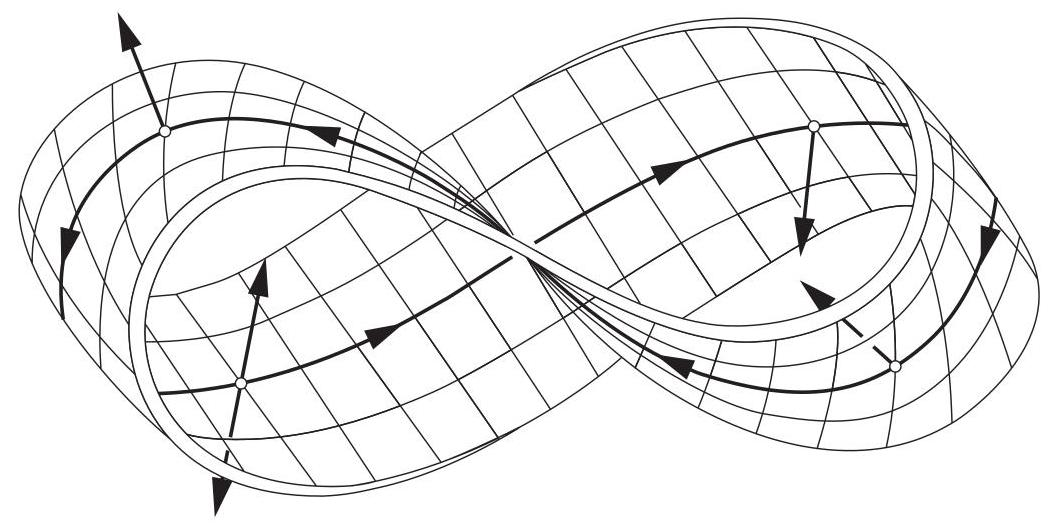
\includegraphics[max width=0.9\textwidth]{images/bo_d4b9jf3ef24c73e0334g_148_255_1518_1054_523_0.jpg}
\captionof{figure}{莫比乌斯带}
\end{center}
\hspace*{3em} 

我们说一个正则曲面是可定向的，如果它能在整个曲面上定义一个可微单位法向量场；选择这样一个场 \(N\) 被称为 \(S\) 的一个定向.

例如，上面提到的莫比乌斯带不是一个可定向曲面.当然，由单个坐标系覆盖的每个曲面(例如，由可微函数的图像表示的曲面)都是平凡可定向的.因此，每个曲面都是局部可定向的，而定向无疑是一个全局属性，因为它涉及到整个曲面.

一个在 \(S\) 上的定向 \(N\) 会在每个切空间 \({T}_{p}\left( S\right)\) , \(p \in  S\) 上诱导一个定向，如下所示.定义一个基 \(\{ v,w\}  \subset  {T}_{p}\left( S\right)\) 为正，如果 \(\langle v \land  w,N\rangle\) 为正.很容易看出， \({T}_{p}\left( S\right)\) 的所有正基的集合是 \({T}_{p}\left( S\right)\) 的一个定向(参见第 1-4 节).

关于定向概念的更多细节在第 2-6 节中给出.然而，对于第 3 章和第 4 章的目的，目前的描述将足够了.

在本章中， \(S\) 将表示一个规则的可定向曲面，其中已选择了一个定向(即，一个可微的单位法向量场 \(N\) )；这将被简单地称为一个具有定向 \(N\) 的曲面 \(S\) .

\begin{definition}{高斯映射}
    设$S\subset{\mathbb{R}}^{3}$为一个具有定向$N$的曲面.映射\(N : S \rightarrow  {\mathbb{R}}^{3}\) 的值在单位球上

\[
{S}^{2} = \left\{  {\left( {x,\mathrm{y},\mathrm{z}}\right)  \in  {\mathbb{R}}^{3};{x}^{2} + {\mathrm{y}}^{2} + {\mathrm{z}}^{2} = 1}\right\}
\]

这样定义的映射 \(N : S \rightarrow  {S}^{2}\) 被称为 \(S\) 的高斯映射(图 3-2).
\end{definition}
高斯映射作用在曲面上，实际就是把每一点的单位法向量移动到原点，将这个点映到其单位法向量的终点.\par

很容易验证高斯映射是可微的. \(N\) 在 \(p \in  S\) 处的微分 \(d{N}_{p}\) 是一个从 \({T}_{p}\left( S\right)\) 到 \({T}_{N\left( p\right) }\left( {S}^{2}\right)\) 的线性映射.由于 \({T}_{p}\left( S\right)\) 和 \({T}_{N\left( p\right) }\left( {S}^{2}\right)\) 是相同的向量空间， \(d{N}_{p}\) 可以看作是 \({T}_{p}\left( S\right)\) 上的一个线性映射.

线性映射 \(d{N}_{p} : {T}_{p}\left( S\right)  \rightarrow  {T}_{p}\left( S\right)\) 的作用如下.对于 \(S\) 中的每个参数化曲线 \(\alpha \left( t\right)\) ，其中 \(\alpha \left( 0\right)  = p\) ，我们考虑球 \({S}^{2}\) 中的参数化曲线 \(N \circ  \alpha \left( t\right)  = N\left( t\right)\) ；这相当于将法向量 \(N\) 限制在曲线 \(\alpha \left( t\right)\) 上.切向量 \({N}^{\prime }\left( 0\right)  = d{N}_{p}\left( {{\alpha }^{\prime }\left( 0\right) }\right)\) 是 \({T}_{p}\left( S\right)\) 中的一个向量(图 3-3).它衡量了在 \(t = 0\) 处，限制在曲线 \(\alpha \left( t\right)\) 上的法向量 \(N\) 的变化率.因此， \(d{N}_{p}\) 衡量了 \(N\) 在 \(p\) 的邻域中如何从 \(N\left( p\right)\) 拉开.在曲线的情况下，这种度量由一个数字给出，即曲率.在曲面的情况下，这种度量由一个线性映射表征.



†在斜体上下文中，字母符号用罗马体而不是斜体表示.



\begin{center}
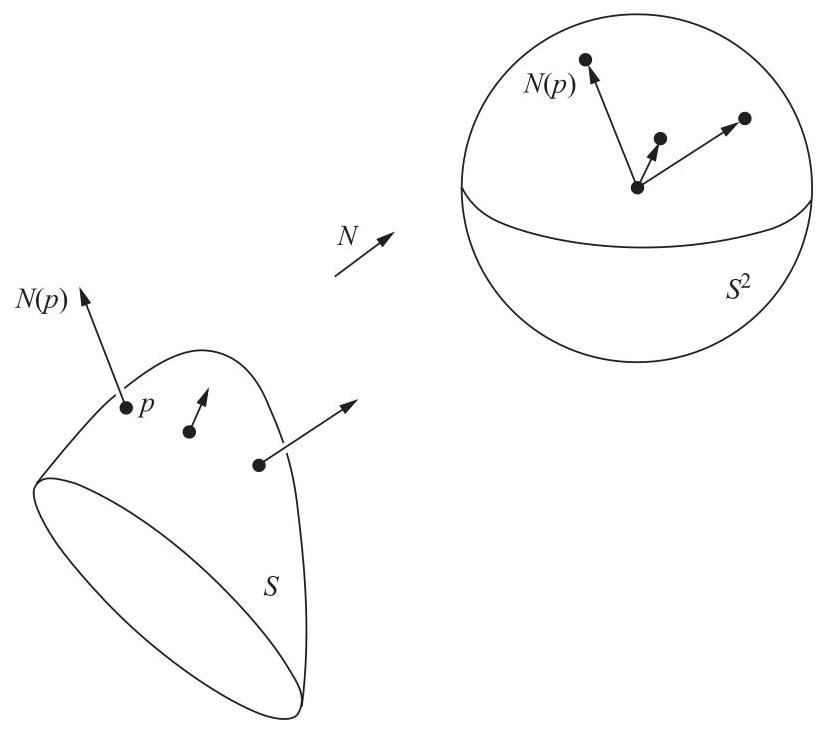
\includegraphics[max width=0.7\textwidth]{images/bo_d4b9jf3ef24c73e0334g_150_369_191_827_729_0.jpg}
\captionof{figure}{高斯映射}
\end{center}
\hspace*{3em} 

\begin{center}
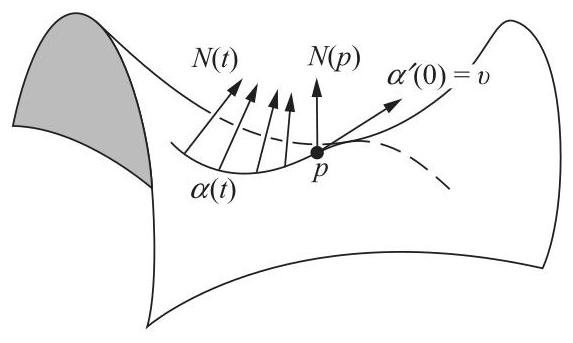
\includegraphics[max width=0.5\textwidth]{images/bo_d4b9jf3ef24c73e0334g_150_197_1044_573_343_0.jpg}
\captionof{figure}{}
\end{center}
\hspace*{3em} 

\begin{instance}
    对于由 \({ax} + {by} + {cz} + d = 0\) 给出的平面 \(P\) ，单位法向量 \(N = \left( {a,b,c}\right) /\sqrt{{a}^{2} + {b}^{2} + {c}^{2}}\) 是常数，因此 \({dN} \equiv  0\) (图 3-4).
\end{instance}

\begin{instance}


\end{instance}



示例 2. 考虑单位球面

\[
{S}^{2} = \left\{  {\left( {x,y,z}\right)  \in  {R}^{3};{x}^{2} + {y}^{2} + {z}^{2} = 1}\right\}  .
\]

如果 \(\alpha \left( t\right)  = \left( {x\left( t\right) ,y\left( t\right) ,z\left( t\right) }\right)\) 是 \({S}^{2}\) 中的参数化曲线，则

\[
{2x}{x}^{\prime } + {2y}{y}^{\prime } + {2z}{z}^{\prime } = 0,
\]

这表明向量 \(\left( {x,y,z}\right)\) 在点 \(\left( {x,y,z}\right)\) 处垂直于球面.因此， \(\bar{N} = \left( {x,y,z}\right)\) 和 \(N = \left( {-x, - y, - z}\right)\) 是 \({S}^{2}\) 中的单位法向量场.我们通过选择 \(N = \left( {-x, - y, - z}\right)\) 作为法向量场来固定 \({S}^{2}\) 中的方向.请注意， \(N\) 指向球心.

\begin{center}
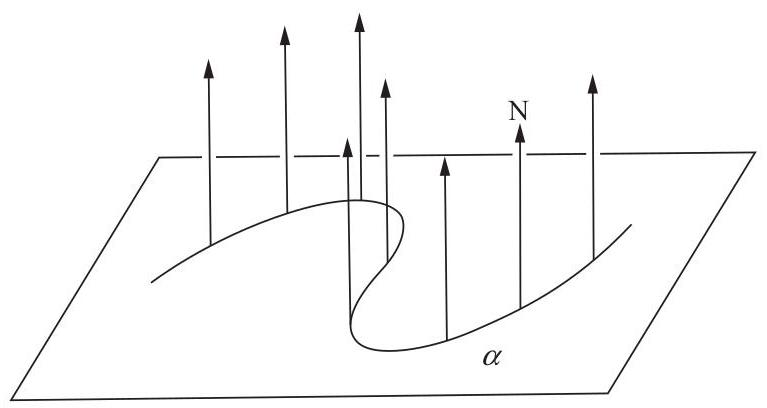
\includegraphics[max width=0.6\textwidth]{images/bo_d4b9jf3ef24c73e0334g_151_381_192_767_408_0.jpg}
\end{center}
\hspace*{3em} 

图 3-4. 平面: \(d{N}_{p} = 0\) .

限制在曲线 \(\alpha \left( t\right)\) 上，法向量

\[
N\left( t\right)  = \left( {-x\left( t\right) , - y\left( t\right) , - z\left( t\right) }\right)
\]

是 \(t\) 的向量函数，因此

\[
{dN}\left( {{x}^{\prime }\left( t\right) ,{y}^{\prime }\left( t\right) ,{z}^{\prime }\left( t\right) }\right)  = {N}^{\prime }\left( t\right)  = \left( {-{x}^{\prime }\left( t\right) , - {y}^{\prime }\left( t\right) , - {z}^{\prime }\left( t\right) }\right) ;
\]

即，对于所有 \(p \in  {S}^{2}\) 和所有 \(v \in  {T}_{p}\left( {S}^{2}\right)\) ，都有 \(d{N}_{p}\left( v\right)  =  - v\) .请注意，通过选择 \(\bar{N}\) 作为法向量场(即，具有相反的方向)，我们将得到 \(d{\bar{N}}_{p}\left( v\right)  = v\) (图 3-5).

\begin{center}
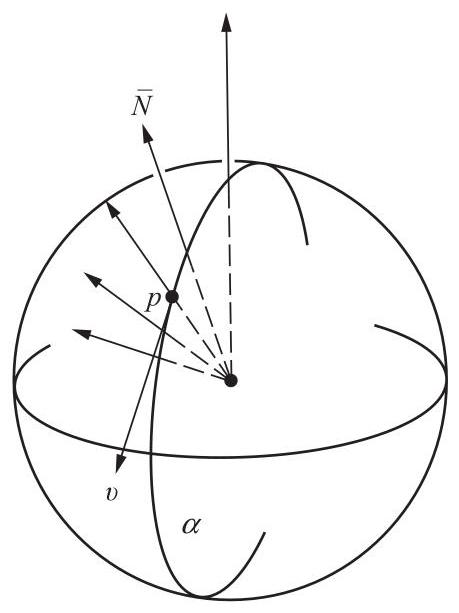
\includegraphics[max width=0.4\textwidth]{images/bo_d4b9jf3ef24c73e0334g_151_176_1499_459_613_0.jpg}
\end{center}
\hspace*{3em} 

图 3-5. 单位球面: \(d{\bar{N}}_{p}\left( v\right)  = v\) .

示例 3. 考虑圆柱体 \(\left\{  {\left( {x,y,z}\right)  \in  {R}^{3};{x}^{2} + {y}^{2} = 1}\right\}\) .通过与前一个示例类似的论证，我们看到 \(\bar{N} = \left( {x,y,0}\right)\) 和 \(N = \left( {-x, - y,0}\right)\) 是 \(\left( {x,y,z}\right)\) 处的单位法向量.我们通过选择 \(N = \left( {-x, - y,0}\right)\) 作为法向量场来固定方向.

通过考虑包含在圆柱体中的曲线 \(\left( {x\left( t\right) ,y\left( t\right) ,z\left( t\right) }\right)\) ，即具有 \({\left( x\left( t\right) \right) }^{2} + {\left( y\left( t\right) \right) }^{2} = 1\) ，我们能够看到，沿着这条曲线， \(N\left( t\right)  = \; \left( {-x\left( t\right) , - y\left( t\right) ,0}\right)\) 因此

\[
{dN}\left( {{x}^{\prime }\left( t\right) ,{y}^{\prime }\left( t\right) ,{z}^{\prime }\left( t\right) }\right)  = {N}^{\prime }\left( t\right)  = \left( {-{x}^{\prime }\left( t\right) , - {y}^{\prime }\left( t\right) ,0}\right) .
\]

我们得出以下结论:如果 \(v\) 是切向圆柱体且平行于 \(z\) 轴的向量，则

\[
{dN}\left( v\right)  = 0 = {0v}
\]

如果 \(w\) 是切向圆柱体且平行于 \({xy}\) 平面的向量，则 \({dN}\left( w\right)  =  - w\) (图 3-6).因此，向量 \(v\) 和 \(w\) 分别是 \({dN}\) 的特征值为 0 和 -1 的特征向量(参见第 3 章附录).

\begin{center}
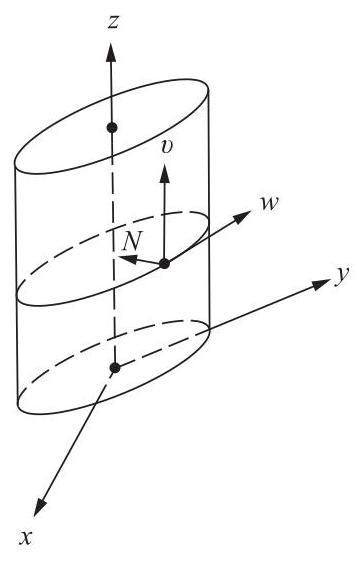
\includegraphics[max width=0.3\textwidth]{images/bo_d4b9jf3ef24c73e0334g_152_197_946_360_565_0.jpg}
\end{center}
\hspace*{3em} 

图 3-6

示例 4. 我们来分析双曲抛物面 \(z = {y}^{2} - {x}^{2}\) 的点 \(p = \left( {0,0,0}\right)\) .为此，我们考虑一个参数化 \(\mathbf{x}\left( {u,v}\right)\) ，其表达式为

\[
\mathbf{x}\left( {u,v}\right)  = \left( {u,v,{v}^{2} - {u}^{2}}\right) ,
\]

并计算法向量 \(N\left( {u,v}\right)\) .我们依次得到

\[
{\mathbf{x}}_{u} = \left( {1,0, - {2u}}\right)
\]

\[
{\mathbf{x}}_{v} = \left( {0,1,{2v}}\right) ,
\]

\[
N = \left( {\frac{u}{\sqrt{{u}^{2} + {v}^{2} + \frac{1}{4}}},\frac{-v}{\sqrt{{u}^{2} + {v}^{2} + \frac{1}{4}}},\frac{1}{2\sqrt{{u}^{2} + {v}^{2} + \frac{1}{4}}}}\right) .
\]

注意到在 \(p = \left( {0,0,0}\right) {\mathbf{x}}_{u}\) 和 \({\mathbf{x}}_{v}\) 处，分别与 \(x\) 和 \(y\) 轴上的单位向量一致.因此，在 \({R}^{3}\) 中，曲线 \(\alpha \left( t\right)  = \mathbf{x}\left( {u\left( t\right) ,v\left( t\right) }\right)\) 在 \(p\) 处的切向量，其中 \(\alpha \left( 0\right)  = p\) ，其坐标为 \(\left( {{u}^{\prime }\left( 0\right) ,{v}^{\prime }\left( 0\right) ,0}\right)\) (图 3-7).将 \(N\left( {u,v}\right)\) 限制到这条曲线上并计算 \({N}^{\prime }\left( 0\right)\) ，我们得到

\[
{N}^{\prime }\left( 0\right)  = \left( {2{u}^{\prime }\left( 0\right) , - 2{v}^{\prime }\left( 0\right) ,0}\right) ,
\]

\begin{center}
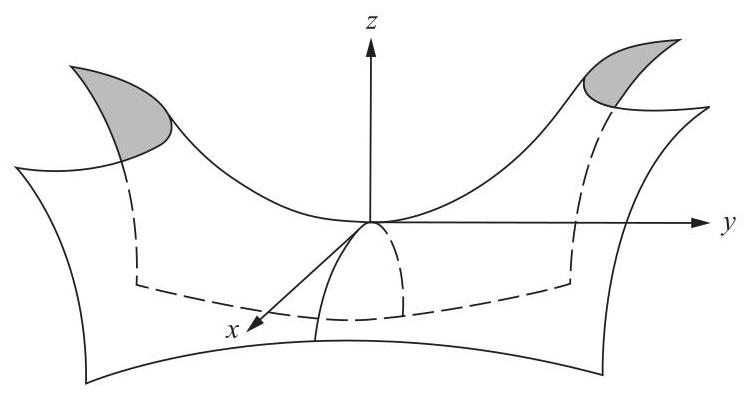
\includegraphics[max width=0.6\textwidth]{images/bo_d4b9jf3ef24c73e0334g_153_393_501_746_393_0.jpg}
\end{center}
\hspace*{3em} 

图 3-7

因此，在 \(p\) 处，

\[
d{N}_{p}\left( {{u}^{\prime }\left( 0\right) ,{v}^{\prime }\left( 0\right) ,0}\right)  = \left( {2{u}^{\prime }\left( 0\right) , - 2{v}^{\prime }\left( 0\right) ,0}\right) .
\]

由此可知，向量 \(\left( {1,0,0}\right)\) 和 \(\left( {0,1,0}\right)\) 分别是 \(d{N}_{p}\) 的特征向量，其特征值为 2 和 -2.

示例 5. 前例的方法应用于抛物面 \(z = {x}^{2} + k{y}^{2},k > 0\) 的点 \(p = \left( {0,0,0}\right)\) ，表明 \(x\) 轴和 \(y\) 轴的单位向量是 \(d{N}_{p}\) 的特征向量，其特征值分别为 2 和 \({2k}\) (假设 \(N\) 指向抛物面所围区域的外部).

关于 \(d{N}_{p}\) 的一个重要事实包含在以下命题中.

命题 1. 高斯映射的微分 \({\mathrm{{dN}}}_{\mathrm{p}} : {\mathrm{T}}_{\mathrm{p}}\left( S\right)  \rightarrow  {\mathrm{T}}_{\mathrm{p}}\left( S\right)\) 是一个自伴随线性映射(参见第 3 章附录).

证明. 由于 \(d{N}_{p}\) 是线性的，只需验证 \({T}_{p}\left( S\right)\) 的基 \(\left\{  {{w}_{1},{w}_{2}}\right\}\) 的 \(\left\langle  {d{N}_{p}\left( {w}_{1}\right) ,{w}_{2}}\right\rangle   = \; \left\langle  {{w}_{1},d{N}_{p}\left( {w}_{2}\right) }\right\rangle\) .设 \(S\) 在 \(p\) 处的参数化为 \(\mathbf{x}\left( {u,v}\right)\) ，其相关的 \({T}_{p}\left( S\right)\) 基为 \(\left\{  {{\mathbf{x}}_{u},{\mathbf{x}}_{v}}\right\}\) .如果 \(S\) 中存在一条参数化曲线 \(\alpha \left( 0\right)  = p\) ，其中 \(\alpha \left( t\right)  = \mathbf{x}\left( {u\left( t\right) ,v\left( t\right) }\right)\) ，则有

\[
d{N}_{p}\left( {{\alpha }^{\prime }\left( 0\right) }\right)  = d{N}_{p}\left( {{\mathbf{x}}_{u}{u}^{\prime }\left( 0\right)  + {\mathbf{x}}_{v}{v}^{\prime }\left( 0\right) }\right)
\]

\[
= {\left. \frac{d}{dt}N\left( u\left( t\right) ,v\left( t\right) \right) \right| }_{t = 0}
\]

\[
= {N}_{u}{u}^{\prime }\left( 0\right)  + {N}_{v}{v}^{\prime }\left( 0\right) ;
\]

特别是， \(d{N}_{p}\left( {\mathbf{x}}_{u}\right)  = {N}_{u}\) 和 \(d{N}_{p}\left( {\mathbf{x}}_{v}\right)  = {N}_{v}\) .因此，要证明 \(d{N}_{p}\) 是自伴的，只需证明

\[
\left\langle  {{N}_{u},{\mathbf{x}}_{v}}\right\rangle   = \left\langle  {{\mathbf{x}}_{u},{N}_{v}}\right\rangle  .
\]

为了看到这一点，分别对 \(\left\langle  {N,{\mathbf{x}}_{u}}\right\rangle   = 0\) 和 \(\left\langle  {N,{\mathbf{x}}_{v}}\right\rangle   = 0\) 关于 \(v\) 和 \(u\) 求导，得到

\[
\left\langle  {{N}_{v},{\mathbf{x}}_{u}}\right\rangle   + \left\langle  {N,{\mathbf{x}}_{uv}}\right\rangle   = 0,
\]

\[
\left\langle  {{N}_{u},{\mathbf{x}}_{v}}\right\rangle   + \left\langle  {N,{\mathbf{x}}_{vu}}\right\rangle   = 0.
\]

因此，

\[
\left\langle  {{N}_{u},{\mathbf{x}}_{v}}\right\rangle   =  - \left\langle  {N,{\mathbf{x}}_{uv}}\right\rangle   = \left\langle  {{N}_{v},{\mathbf{x}}_{u}}\right\rangle  . \tag{Q.E.D.}
\]

由于 \(d{N}_{p} : {T}_{p}\left( S\right)  \rightarrow  {T}_{p}\left( S\right)\) 是一个自伴线性映射，我们可以将 \(d{N}_{p}\) 与 \({T}_{p}\left( S\right)\) 中的一个二次型 \(Q\) 相关联，该二次型由 \(Q\left( v\right)  = \left\langle  {d{N}_{p}\left( v\right) ,v}\right\rangle\) 定义， \(v \in  {T}_{p}\left( S\right)\) (参见第 3 章附录).为了获得这个二次型的几何解释，我们需要一些定义.出于稍后将变得清晰的原因，我们将使用二次型 \(- Q\) .

定义 2. 在 \({\mathrm{T}}_{\mathrm{p}}\left( S\right)\) 中由 \({\mathrm{{II}}}_{\mathrm{p}}\left( \mathrm{v}\right)  = \; - \left\langle  {{\mathrm{{dN}}}_{\mathrm{p}}\left( \mathrm{v}\right) ,\mathrm{v}}\right\rangle\) 定义的二次型 \({\mathrm{{II}}}_{\mathrm{p}}\) 称为 \(S\) 在 \(\mathrm{p}\) 处的二阶基本形式.

定义 3. 令 \(\mathrm{C}\) 为 \(S\) 中通过 \(\mathrm{p} \in  S\) 的一条正则曲线， \(\mathrm{k}\) 为 \(\mathrm{C}\) 在 \(\mathrm{p}\) 处的曲率，以及 \(\cos \theta  = \langle N,N\rangle\) ，其中 \(N\) 是 \(\mathrm{C}\) 的法向量，而 \(N\) 是 \(S\) 在 \(\mathrm{p}\) 处的法向量.则数 \({\mathrm{k}}_{N} = \mathrm{k}\cos \theta\) 称为 \(\mathrm{C} \subset  S\) 在 \(\mathrm{p}\) 处的法曲率.

换句话说， \({k}_{n}\) 是向量 \({kn}\) 在曲面在 \(p\) 处的法线上的投影的长度，其符号由 \(S\) 在 \(p\) 处的方向 \(N\) 给出(图 3-8).

\begin{center}
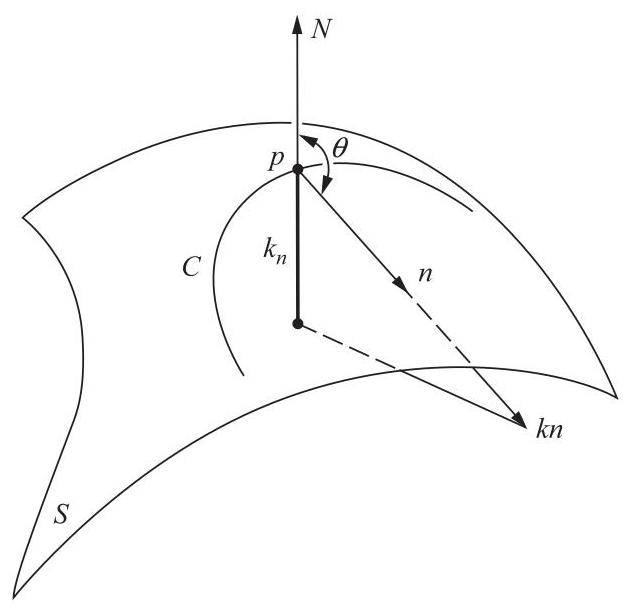
\includegraphics[max width=0.5\textwidth]{images/bo_d4b9jf3ef24c73e0334g_154_198_1500_630_613_0.jpg}
\end{center}
\hspace*{3em} 

注记.法曲率 \(C\) 不依赖于 \(C\) 的方向，但随着曲面方向的变化而改变符号.

为了给出二阶基本形式 \(I{I}_{p}\) 的解释，考虑一条由 \(\alpha \left( s\right)\) 参数化的正则曲线 \(C \subset  S\) ，其中 \(s\) 是 \(C\) 的弧长，并且有 \(\alpha \left( 0\right)  = p\) .如果我们用 \(N\left( s\right)\) 表示法向量 \(N\) 在曲线 \(\alpha \left( s\right)\) 上的限制，我们有 \(\left\langle  {N\left( s\right) ,{\alpha }^{\prime }\left( s\right) }\right\rangle   = 0\) .因此，

\[
\left\langle  {N\left( s\right) ,{\alpha }^{\prime \prime }\left( s\right) }\right\rangle   =  - \left\langle  {{N}^{\prime }\left( s\right) ,{\alpha }^{\prime }\left( s\right) }\right\rangle  .
\]

因此，

\[
{\Pi }_{p}\left( {{\alpha }^{\prime }\left( 0\right) }\right)  =  - \left\langle  {d{N}_{p}\left( {{\alpha }^{\prime }\left( 0\right) }\right) ,{\alpha }^{\prime }\left( 0\right) }\right\rangle
\]

\[
=  - \left\langle  {{N}^{\prime }\left( 0\right) ,{\alpha }^{\prime }\left( 0\right) }\right\rangle   = \left\langle  {N\left( 0\right) ,{\alpha }^{\prime \prime }\left( 0\right) }\right\rangle
\]

\[
= \langle N,{kn}\rangle \left( p\right)  = {k}_{n}\left( p\right) .
\]

换句话说，单位向量 \(v \in  {T}_{p}\left( S\right)\) 的第二基本形式 \(I{I}_{p}\) 的值等于通过 \(p\) 且与 \(v\) 相切的正則曲線的法曲率.特别地，我们得到了以下结果.

命题 2 (Meusnier).曲面 S 上在给定点 \(\mathrm{p} \in  S\) 具有相同切线的全部曲线在该点具有相同的法曲率.

上述命题允许我们谈论在 \(p\) 处沿给定方向的法曲率.使用以下术语很方便.给定一个单位向量 \(v \in  {T}_{p}\left( S\right)\) ， \(S\) 与包含 \(v\) 和 \(N\left( p\right)\) 的平面相交，称为 \(S\) 在 \(p\) 处沿 \(v\) 的法截线(图 3-9).在 \(p\) 的邻域中， \(S\) 在 \(p\) 处的法截线是 \(S\) 上的一个正则平面曲线，其在 \(p\) 处的法向量 \(n\) 为 \(\pm  N\left( p\right)\) 或零；因此其曲率等于沿 \(v\) 在 \(p\) 处的法曲率的绝对值.使用此术语，上述命题表明曲线 \(\alpha \left( s\right)\) 在 \(p\) 处的法曲率的绝对值等于 \(S\) 在 \(p\) 处沿 \({\alpha }^{\prime }\left( 0\right)\) 的法截线的曲率.

\begin{center}
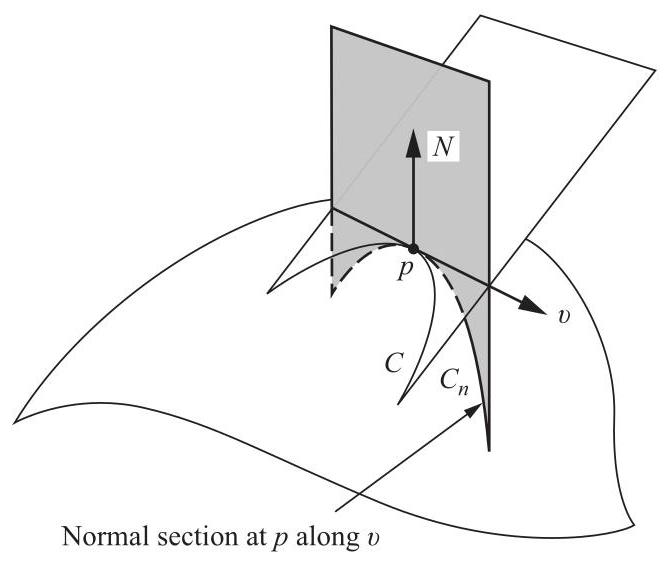
\includegraphics[max width=0.6\textwidth]{images/bo_d4b9jf3ef24c73e0334g_155_180_1544_665_562_0.jpg}
\end{center}
\hspace*{3em} 

图 3-9.Meusnier 定理: \(C\) 和 \({C}_{n}\) 在 \(p\) 处沿 \(v\) 具有相同的法曲率.

例 6.考虑通过将曲线 \(z = {y}^{4}\) 绕 \(z\) 轴旋转得到的旋转曲面(图 3-10).我们将证明在 \(p = \left( {0,0,0}\right)\) 处微分 \(d{N}_{p} = 0\) .为了看到这一点，我们观察到曲线 \(z = {y}^{4}\) 在 \(p\) 处的曲率为零.此外，由于 \({xy}\) 平面是曲面在 \(p\) 处的切平面，法向量 \(N\left( p\right)\) 平行于 \(z\) 轴.因此，在 \(p\) 处的任何法截线都是通过旋转曲线 \(z = {y}^{4}\) 得到的；因此，其曲率为零.由此得出，在 \(p\) 处所有法曲率都为零，因此 \(d{N}_{p} = 0\) .

\begin{center}
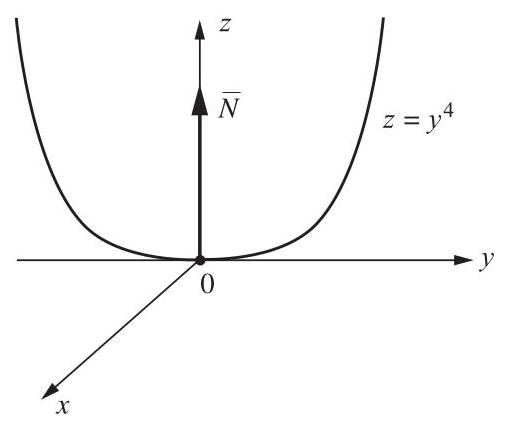
\includegraphics[max width=0.4\textwidth]{images/bo_d4b9jf3ef24c73e0334g_156_194_721_505_430_0.jpg}
\end{center}
\hspace*{3em} 

图 3-10

例 7.在例 1 的平面中，所有法截线都是直线；因此，所有法曲率都为零.因此，第二基本形式在所有点处都恒为零.这与 \({dN} \equiv  0\) 的事实一致.

在例 2 的球面 \({S}^{2}\) 中，取 \(N\) 作为方向，通过点 \(p \in  {S}^{2}\) 的法截线是半径为 1 的圆(图 3-11).因此，所有法曲率都等于 1，并且对于所有 \(p \in  {S}^{2}\) 和所有满足 \(\left| v\right|  = 1\) 的 \(v \in  {T}_{p}\left( S\right)\) ，第二基本形式为 \({\Pi }_{p}\left( v\right)  = 1\) .

\begin{center}
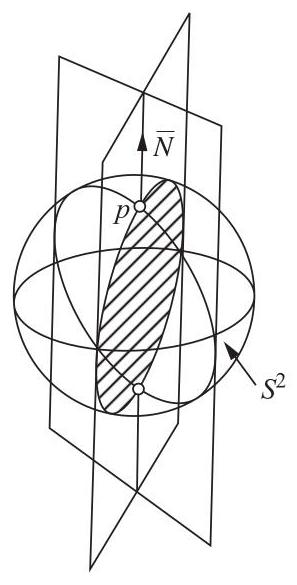
\includegraphics[max width=0.2\textwidth]{images/bo_d4b9jf3ef24c73e0334g_156_196_1524_297_585_0.jpg}
\end{center}
\hspace*{3em} 

图 3-11.球面上的法截线.

在例 3 的圆柱体中，在点 \(p\) 处的法截线从垂直于圆柱体轴的圆变化到平行于圆柱体轴的直线，经过一系列椭圆(图 3-12).因此，法曲率从 1 变化到 0.从几何上不难看出，1 是 \(p\) 处法曲率的最大值，0 是最小值.

\begin{center}
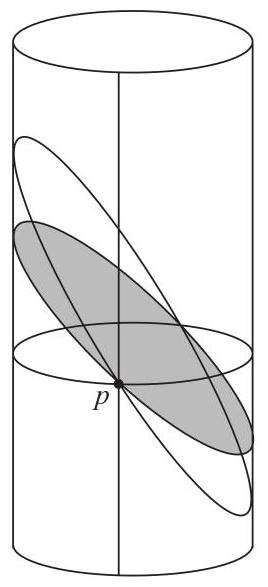
\includegraphics[max width=0.2\textwidth]{images/bo_d4b9jf3ef24c73e0334g_157_180_463_268_587_0.jpg}
\end{center}
\hspace*{3em} 

图 3-12.圆柱体上的法截线.

然而，将附录第 3 章二次型定理应用于此，可以得到一个简单的证明.事实上，正如我们在例 3 中所见，向量 \(w\) 和 \(v\) (分别对应于法曲率 1 和 0 的方向)是 \(d{N}_{p}\) 的特征向量，其特征值为 -1 和 0.因此，二次基本形式在这两个向量上取极值，正如我们所声称的.请注意，此过程允许我们检查这些极值是否为 1 和 0.

我们留给读者分析例 4 中双曲抛物面在点 \(p = \; \left( {0,0,0}\right)\) 处的法截线.

让我们回到线性映射 \(d{N}_{p}\) .附录第 3 章的定理表明，对于每个 \(p \in  S\) ，都存在一个 \({T}_{p}\left( S\right)\) 的标准正交基 \(\left\{  {{e}_{1},{e}_{2}}\right\}\) ，使得 \(d{N}_{p}\left( {e}_{1}\right)  =  - {k}_{1}{e}_{1},d{N}_{p}\left( {e}_{2}\right)  =  - {k}_{2}{e}_{2}\) .此外， \({k}_{1}\) 和 \({k}_{2} \; \left( {{k}_{1} \geq  {k}_{2}}\right)\) 是二次基本形式 \(I{I}_{p}\) 在 \({T}_{p}\left( S\right)\) 单位圆上的限制的极大值和极小值；也就是说，它们是 \(p\) 处法曲率的极值.

定义 4. 最大法曲率 \({\mathrm{k}}_{1}\) 和最小法曲率 \({\mathrm{k}}_{2}\) 称为 \(\mathrm{p}\) 处的**主曲率**；相应的方向，即由特征向量 \({\mathrm{e}}_{1},{\mathrm{e}}_{2}\) 给出的方向，称为 p 处的**主方向**.

例如，在平面上，所有点上的所有方向都是主方向.在球面上也是如此.在这两种情况下，这是因为每个点处的二次基本形式，限制在单位向量上，是常数(参见例 7)；因此，所有方向都是法曲率的极值方向.

在例 3 的圆柱体中，向量 \(v\) 和 \(w\) 给出了 \(p\) 处的主方向，分别对应于主曲率 0 和 1.在例 4 的双曲抛物面中， \(x\) 和 \(y\) 轴沿着主方向，主曲率分别为 -2 和 2.

定义 5. 如果 \(S\) 上的一条正则连通曲线 \(\mathrm{C}\) 使得对于所有 \(\mathrm{p} \in  \mathrm{C}\) ， \(\mathrm{C}\) 的切线是 \(\mathrm{p}\) 处的主方向，则称 \(\mathrm{C}\) 是 \(S\) 的**曲率线**.

命题 3 (Olinde Rodrigues). \(S\) 上的一条连通正则曲线 \(\mathrm{C}\) 是 \(S\) 的曲率线的充要条件是

\[
{N}^{\prime }\left( \mathrm{t}\right)  = \lambda \left( \mathrm{t}\right) {\alpha }^{\prime }\left( \mathrm{t}\right) ,
\]

对于 \(\mathrm{C}\) 的任何参数化 \(\alpha \left( \mathrm{t}\right)\) ，其中 \(N\left( \mathrm{t}\right)  = N \circ  \alpha \left( \mathrm{t}\right)\) 和 \(\lambda \left( \mathrm{t}\right)\) 是 \(\mathrm{t}\) 的可微函数.在这种情况下， \(- \lambda \left( \mathrm{t}\right)\) 是沿 \({\alpha }^{\prime }\left( \mathrm{t}\right)\) 的(主)曲率.

证明.只需观察到，如果 \({\alpha }^{\prime }\left( t\right)\) 包含在主方向中，则 \({\alpha }^{\prime }\left( t\right)\) 是 \({dN}\) 的特征向量，并且

\[
{dN}\left( {{\alpha }^{\prime }\left( t\right) }\right)  = {N}^{\prime }\left( t\right)  = \lambda \left( t\right) {\alpha }^{\prime }\left( t\right) .
\]

反之亦然.Q.E.D.

了解 \(p\) 处的主曲率可以让我们轻松计算 \({T}_{p}\left( S\right)\) 中给定方向上的法曲率.事实上，设 \(v \in  {T}_{p}\left( S\right)\) 且 \(\left| v\right|  = 1\) .由于 \({e}_{1}\) 和 \({e}_{2}\) 构成 \({T}_{p}\left( S\right)\) 的一个标准正交基，我们有

\[
v = {e}_{1}\cos \theta  + {e}_{2}\sin \theta
\]

其中 \(\theta\) 是从 \({e}_{1}\) 到 \(v\) 在 \({T}_{p}\left( S\right)\) 方向上的角度.沿 \(v\) 的法曲率 \({k}_{n}\) 由下式给出

\[
{k}_{n} = I{I}_{p}\left( v\right)  =  - \left\langle  {d{N}_{p}\left( v\right) ,v}\right\rangle
\]

\[
=  - \left\langle  {d{N}_{p}\left( {{e}_{1}\cos \theta  + {e}_{2}\sin \theta }\right) ,{e}_{1}\cos \theta  + {e}_{2}\sin \theta }\right\rangle
\]

\[
= \left\langle  {{e}_{1}{k}_{1}\cos \theta  + {e}_{2}{k}_{2}\sin \theta ,{e}_{1}\cos \theta  + {e}_{2}\sin \theta }\right\rangle
\]

\[
= {k}_{1}{\cos }^{2}\theta  + {k}_{2}{\sin }^{2}\theta \text{ . }
\]

最后一个表达式经典地称为欧拉公式；实际上，它只是二次基本形式在基 \(\left\{  {{e}_{1},{e}_{2}}\right\}\) 上的表达式.

给定一个二维向量空间的线性映射 \(A : V \rightarrow  V\) 和一个基 \(\left\{  {{v}_{1},{v}_{2}}\right\}\) 的 \(V\) ，我们回忆

\[
\text{ determinant of }A = {a}_{11}{a}_{22} - {a}_{12}{a}_{21},\;\text{ trace of }A = {a}_{11} + {a}_{22}\text{ , }
\]

其中 \(\left( {a}_{ij}\right)\) 是基 \(\left\{  {{v}_{1},{v}_{2}}\right\}\) 中 \(A\) 的矩阵.已知这些数不依赖于基 \(\left\{  {{v}_{1},{v}_{2}}\right\}\) 的选择，因此附属于线性映射 \(A\) .

在我们的例子中， \({dN}\) 的行列式是主曲率 \(\left( {-{k}_{1}}\right) \left( {-{k}_{2}}\right)  = {k}_{1}{k}_{2}\) 的乘积，而 \({dN}\) 的迹是主曲率之和的负 \(- \left( {{k}_{1} + {k}_{2}}\right)\) .如果我们改变曲面的方向，行列式不变(这里偶数维是至关重要的)；然而，迹改变符号.

定义 6. 令 \(\mathrm{p} \in  S\) ，令 \({\mathrm{{dN}}}_{\mathrm{p}} : {\mathrm{T}}_{\mathrm{p}}\left( S\right)  \rightarrow  {\mathrm{T}}_{\mathrm{p}}\left( S\right)\) 为高斯映射的微分. \({\mathrm{{dN}}}_{\mathrm{p}}\) 的行列式是 \(S\) 在 \(\mathrm{p}\) 处的高斯曲率 \(\mathrm{K}\) . \({\mathrm{{dN}}}_{\mathrm{p}}\) 的迹的负一半称为 S 在 p 处 的平均曲率 H.

用主曲率表示，我们可以写出

\[
K = {k}_{1}{k}_{2},\;H = \frac{{k}_{1} + {k}_{2}}{2}.
\]

定义 7. 曲面 \(S\) 的一个点称为

1. 椭圆点，如果 \(\det \left( {\mathrm{{dN}}}_{\mathrm{p}}\right)  > 0\) .

2. 双曲点，如果 \(\det \left( {\mathrm{{dN}}}_{\mathrm{p}}\right)  < 0\) .

3. 抛物点，如果 \(\det \left( {\mathrm{{dN}}}_{\mathrm{p}}\right)  = 0\) ，且 \({\mathrm{{dN}}}_{\mathrm{p}} \neq  0\) .

4. 平点，如果 \({\mathrm{{dN}}}_{\mathrm{p}} = 0\) .

显然，这种分类不依赖于方向的选择.

在椭圆点处，高斯曲率为正.两个主曲率符号相同，因此通过该点的所有曲线的法向量都指向切平面同侧.球面的点是椭圆点.抛物面 \(z = {x}^{2} + k{y}^{2},k > 0\) 的点 \(\left( {0,0,0}\right)\) (参见示例 5)也是椭圆点.

在双曲点处，高斯曲率为负.主曲率符号相反，因此存在通过 \(p\) 的曲线，其在 \(p\) 处的法向量指向双曲抛物面 \(z = {y}^{2} - {x}^{2}\) (参见示例 4)的切平面 \(\left( {0,0,0}\right)\) 的任意一侧.

在抛物点处，高斯曲率为零，但其中一个主曲率不为零.圆柱体(参见示例 3)的点是抛物点.

最后，在平面点处，所有主曲率都为零.平面的点显然满足此条件.平面点的非平凡示例在示例 6 中给出.

定义 8. 如果在 \(\mathrm{p} \in  S,{\mathrm{k}}_{1} = {\mathrm{k}}_{2}\) 处，则 \(\mathrm{p}\) 被称为 \(S\) 的脐点；特别地，平面点 \(\left( {{\mathrm{k}}_{1} = {\mathrm{k}}_{2} = 0}\right)\) 是脐点.

球体和平面上的所有点都是脐点.使用示例 6 的方法，我们可以验证抛物面 \(z = {x}^{2} + {y}^{2}\) 上的点 \(\left( {0,0,0}\right)\) 是一个(非平面)脐点.

现在我们将证明一个有趣的结论:唯一完全由脐点组成的曲面本质上是球体和平面.

命题 4. 如果一个连通曲面 \(S\) 的所有点都是脐点，则 \(S\) 包含在一个球体或一个平面中.

证明. 令 \(p \in  S\) ，并令 \(\mathbf{x}\left( {u,v}\right)\) 为 \(S\) 在 \(p\) 处的一个参数化，使得坐标邻域 \(V\) 是连通的.

由于每个 \(q \in  V\) 都是脐点，对于 \({T}_{q}\left( S\right)\) 中的任何向量 \(w = \; {a}_{1}{\mathbf{x}}_{u} + {a}_{2}{\mathbf{x}}_{v}\) ，我们有:

\[
{dN}\left( w\right)  = \lambda \left( q\right) w
\]

其中 \(\lambda  = \lambda \left( q\right)\) 是 \(V\) 中的一个实可微函数.

我们首先证明 \(\lambda \left( q\right)\) 在 \(V\) 中是常数.为此，我们将上述方程写成:

\[
{N}_{u}{a}_{1} + {N}_{v}{a}_{2} = \lambda \left( {{\mathbf{x}}_{u}{a}_{1} + {\mathbf{x}}_{v}{a}_{2}}\right) ;
\]

因此，由于 \(w\) 是任意的，

\[
{N}_{u} = \lambda {\mathbf{x}}_{u}
\]

\[
{N}_{v} = \lambda {\mathbf{x}}_{v}
\]

对第一个方程在 \(v\) 上求导，对第二个方程在 \(u\) 上求导，然后减去所得方程，我们得到:

\[
{\lambda }_{u}{\mathbf{x}}_{v} - {\lambda }_{v}{\mathbf{x}}_{u} = 0
\]

由于 \({\mathbf{x}}_{u}\) 和 \({\mathbf{x}}_{v}\) 线性无关，我们得出结论:

\[
{\lambda }_{u} = {\lambda }_{v} = 0
\]

对于所有 \(q \in  V\) .由于 \(V\) 是连通的， \(\lambda\) 在 \(V\) 中是常数，正如我们所声称的.

如果 \(\lambda  \equiv  0,{N}_{u} = {N}_{v} = 0\) 且因此 \(N = {N}_{0} =\) 在 \(V\) 中为常数.因此， \({\left\langle  \mathbf{x}\left( u,v\right) ,{N}_{0}\right\rangle  }_{u} = {\left\langle  \mathbf{x}\left( u,v\right) ,{N}_{0}\right\rangle  }_{v} = 0\) ；所以，

\[
\left\langle  {\mathbf{x}\left( {u,v}\right) ,{N}_{0}}\right\rangle   = \text{ const., }
\]

且 \(V\) 的所有点 \(\mathbf{x}\left( {u,v}\right)\) 属于一个平面.

如果 \(\lambda  \neq  0\) ，则点 \(\mathbf{x}\left( {u,v}\right)  - \left( {1/\lambda }\right) N\left( {u,v}\right)  = \mathbf{y}\left( {u,v}\right)\) 固定，因为

\[
{\left( \mathbf{x}\left( u,v\right)  - \frac{1}{\lambda }N\left( u,v\right) \right) }_{u} = {\left( \mathbf{x}\left( u,v\right)  - \frac{1}{\lambda }N\left( u,v\right) \right) }_{v} = 0.
\]

因为

\[
{\left| \mathbf{x}\left( u,v\right)  - \mathbf{y}\right| }^{2} = \frac{1}{{\lambda }^{2}},
\]

\(V\) 的所有点都包含在以 \(\mathbf{y}\) 为中心、 \(1/\left| \lambda \right|\) 为半径的球内.

这在局部上证明了该命题，即对于点 \(p \in  S\) 的一个邻域.为了完成证明，我们注意到，由于 \(S\) 是连通的，给定任何其他点 \(r \in  S\) ，存在一条连续曲线 \(\alpha  : \left\lbrack  {0,1}\right\rbrack   \rightarrow  S\) ，使得 \(\alpha \left( 0\right)  = p\) ， \(\alpha \left( 1\right)  = r\) .对于这条曲线的每个点 \(\alpha \left( t\right)  \in  S\) ，存在 \(S\) 中的一个邻域 \({V}_{t}\) ，该邻域包含在一个球或一个平面内，并且 \({\alpha }^{-1}\left( {V}_{t}\right)\) 是 \(\left\lbrack  {0,1}\right\rbrack\) 的一个开区间.并集 \(\bigcup {\alpha }^{-1}\left( {V}_{t}\right) ,t \in  \left\lbrack  {0,1}\right\rbrack\) 覆盖了 \(\left\lbrack  {0,1}\right\rbrack\) ，由于 \(\left\lbrack  {0,1}\right\rbrack\) 是一个闭区间，它被族 \(\left\{  {{\alpha }^{-1}\left( {V}_{t}\right) }\right\}\) 的有限多个元素覆盖(参见 Heine-Borel 定理，第 2 章附录命题 6).因此， \(\alpha \left( \left\lbrack  {0,1}\right\rbrack  \right)\) 被有限个邻域 \({V}_{t}\) 覆盖.

如果其中一个邻域的点在平面上，那么所有其他点也将在同一平面上.由于 \(r\) 是任意的， \(S\) 的所有点都属于这个平面.

如果其中一个邻域的点在球面上，同样的论证表明 \(S\) 上的所有点都属于一个球面，这就完成了证明.证毕.

定义 9. 令 \(\mathrm{p}\) 为 S 中的一个点. \(S\) 在 \(\mathrm{p}\) 处的一个渐近方向是 \({\mathrm{T}}_{\mathrm{p}}\left( S\right)\) 的一个方向，其法向曲率为零. \(S\) 的一个渐近曲线是正则连通曲线 \(\mathrm{C} \subset  S\) ，使得对于每个 \(\mathrm{p} \in  \mathrm{C}\) ， \(\mathrm{C}\) 在 \(\mathrm{p}\) 处的切线是一个渐近方向.

从定义可以立即得出，在椭圆点处没有渐近方向.

通过 Dupin 示性曲面可以对渐近方向进行有用的几何解释，我们现在将对此进行描述.

设 \(p\) 为 \(S\) 中的一点.点 \(p\) 处的 Dupin 指示曲面是 \(w\) 组成的向量集合，这些向量属于 \({T}_{p}\left( S\right)\) ，并且满足 \({\Pi }_{p}\left( w\right)  =  \pm  1\) .

为了更方便地写出 Dupin 指示曲面的方程，设 \(\left( {\xi ,\eta }\right)\) 为在 orthonormal basis \(\left\{  {{e}_{1},{e}_{2}}\right\}\) 下点 \({T}_{p}\left( S\right)\) 的笛卡尔坐标，其中 \({e}_{1}\) 和 \({e}_{2}\) 是 \(d{N}_{p}\) 的特征向量.给定 \(w \in  {T}_{p}\left( S\right)\) ，设 \(\rho\) 和 \(\theta\) 为由 \(w = {\rho v}\) 定义的“极坐标”，其中 \(\left| v\right|  = 1\) 和 \(v = {e}_{1}\cos \theta  + \; {e}_{2}\sin \theta\) ，如果 \(\rho  \neq  0\) .根据欧拉公式，

\[
\pm  1 = {I}_{p}\left( w\right)  = {p}^{2}{I}_{p}\left( v\right)
\]

\[
= {k}_{1}{\rho }^{2}{\cos }^{2}\theta  + {k}_{2}{\rho }^{2}{\sin }^{2}\theta
\]

\[
= {k}_{1}{\xi }^{2} + {k}_{2}{\eta }^{2},
\]

其中 \(w = \xi {e}_{1} + \eta {e}_{2}\) .因此，Dupin 指示曲面上点的坐标 \(\left( {\xi ,\eta }\right)\) 满足方程

\[
{k}_{1}{\xi }^{2} + {k}_{2}{\eta }^{2} =  \pm  1 \tag{1}
\]

因此，Dupin 指示曲面是 \({T}_{p}\left( S\right)\) 中的圆锥曲线的并集.我们注意到，沿由 \(w\) 确定的方向的法曲率为 \({k}_{n}\left( v\right)  = {I}_{p}\left( v\right)  = \; \pm  \left( {1/{\rho }^{2}}\right)\) .

对于椭圆点，Dupin 指示曲面是一个椭圆( \(\left( {k}_{1}\right.\) 和 \({k}_{2}\) 同号)；如果该点是脐点非平面点 \(\left( {{k}_{1} = {k}_{2} \neq  0}\right)\) ，则该椭圆退化为圆.

对于双曲点， \({k}_{1}\) 和 \({k}_{2}\) 异号.因此，Dupin 指示曲面由两条具有共同渐近线对的双曲线组成(图 3-13).沿渐近线方向，法曲率为零；因此它们是渐近方向.这证明了术语的合理性，并表明双曲点恰好有两个渐近方向.

\begin{center}
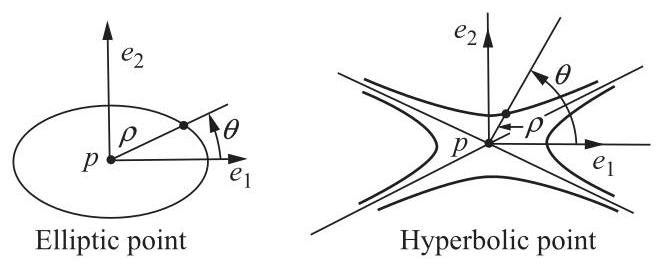
\includegraphics[max width=0.5\textwidth]{images/bo_d4b9jf3ef24c73e0334g_162_456_1245_659_265_0.jpg}
\end{center}
\hspace*{3em} 

图 3-13.Dupin 指示曲面.

对于抛物点，一个主曲率为零，Dupin 指示曲面退化为一对平行线.这些线的共同方向是给定点的唯一渐近方向.

在第 3-3 节的示例 5 中，我们将展示 Dupin 指示曲面的一个有趣性质.

与渐近方向的概念密切相关的是共轭方向的概念，我们现在将定义它.

定义 10.设 \(\mathrm{p}\) 为曲面 \(S\) 上的一个点.两个非零向量 \({\mathrm{w}}_{1},{\mathrm{w}}_{2} \in  {\mathrm{T}}_{\mathrm{p}}\left( S\right)\) 是共轭的，如果 \(\left\langle  {{\mathrm{{dN}}}_{\mathrm{p}}\left( {\mathrm{w}}_{1}\right) ,{\mathrm{w}}_{2}}\right\rangle   = \left\langle  {{\mathrm{w}}_{1},{\mathrm{{dN}}}_{\mathrm{p}}\left( {\mathrm{w}}_{2}\right) }\right\rangle   = 0\) .

\(\mathrm{p}\) 处的两个方向 \({\mathrm{r}}_{1},{\mathrm{r}}_{2}\) 是共轭的，如果 \(a\) 非零向量 \({\mathrm{w}}_{1},{\mathrm{\;w}}_{2}\) 平行于 \({\mathrm{r}}_{1}\) 和 \({\mathrm{r}}_{2}\) 分别是共轭的.

易于检查共轭方向的定义不依赖于在 \({r}_{1}\) 和 \({r}_{2}\) 上选择向量 \({w}_{1}\) 和 \({w}_{2}\) .

从定义可知，主方向是共轭的，渐近方向与其自身共轭.此外，在非平面脐点，每对正交方向都是一对共轭方向，而在平面脐点，每个方向都与其他任何方向共轭.

我们假设 \(p \in  S\) 不是脐点，令 \(\left\{  {{e}_{1},{e}_{2}}\right\}\) 为由 \(d{N}_{p}\left( {e}_{1}\right)  =  - {k}_{1}{e}_{1},d{N}_{p}\left( {e}_{2}\right)  = \; - {k}_{2}{e}_{2}\) 确定的 \({T}_{p}\left( S\right)\) 的标准正交基.令 \(\theta\) 和 \(\varphi\) 为一对方向 \({r}_{1}\) 和 \({r}_{2}\) 与 \({e}_{1}\) 所成的角度.我们声称 \({r}_{1}\) 和 \({r}_{2}\) 共轭当且仅当

\[
{k}_{1}\cos \theta \cos \varphi  =  - {k}_{2}\sin \theta \sin \varphi . \tag{2}
\]

事实上， \({r}_{1}\) 和 \({r}_{2}\) 共轭当且仅当向量

\[
{w}_{1} = {e}_{1}\cos \theta  + {e}_{2}\sin \theta ,\;{w}_{2} = {e}_{1}\cos \varphi  + {e}_{2}\sin \varphi
\]

共轭.因此，

\[
0 = \left\langle  {d{N}_{p}\left( {w}_{1}\right) ,{w}_{2}}\right\rangle   =  - {k}_{1}\cos \theta \cos \varphi  - {k}_{2}\sin \theta \sin \varphi .
\]

因此，条件 (2) 得出.

当 \({k}_{1}\) 和 \({k}_{2}\) 都非零时(即 \(p\) 是椭圆点或双曲点)，条件 (2) 导致在 \(p\) 处的 Dupin 示性曲面在几何上构造共轭方向.我们将描述在椭圆点处的构造，在双曲点处的情况类似.令 \(r\) 为通过 \({T}_{p}\left( S\right)\) 原点的直线，并考虑 \(r\) 与 Dupin 示性曲面的交点 \({q}_{1},{q}_{2}\) (图 3-14).在 \(p\) 处的 Dupin 示性曲线的切线

\begin{center}
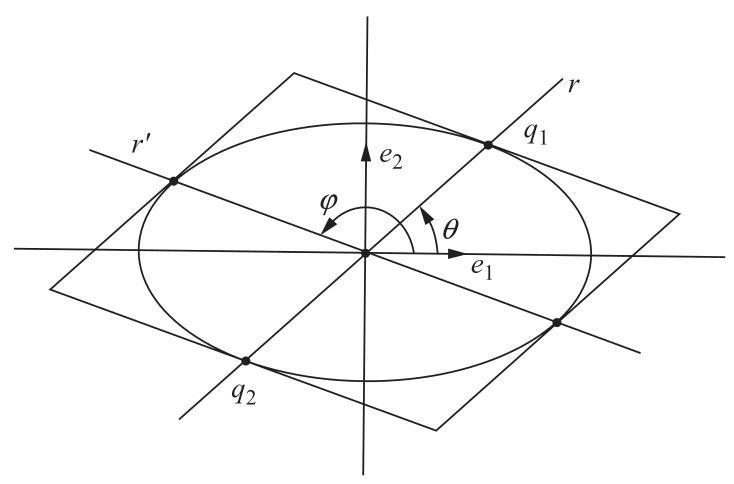
\includegraphics[max width=0.6\textwidth]{images/bo_d4b9jf3ef24c73e0334g_163_400_1560_734_484_0.jpg}
\end{center}
\hspace*{3em} 

图 3-14. 共轭方向的构造.

在 \({q}_{1}\) 和 \({q}_{2}\) 处的 Dupin 示性曲面平行，并且它们的共同方向 \({r}^{\prime }\) 与 \(r\) 共轭.我们将把这些论断的证明留给练习(练习 12).

\exerciseline

1. 证明在双曲点处，主方向平分渐近方向.

2. 证明如果一个曲面沿一条曲线与一个平面相切，那么这条曲线上的点要么是抛物点要么是平面点.

3. 令 \(C \subset  S\) 为曲面 \(S\) 上具有高斯曲率 \(K > 0\) 的一条正则曲线.证明 \(p\) 处 \(C\) 的曲率 \(k\) 满足

\[
\left| k\right|  \geq  \min \left( {\left| {k}_{1}\right| ,\left| {k}_{2}\right| }\right)
\]

其中 \({k}_{1}\) 和 \({k}_{2}\) 是 \(S\) 在 \(p\) 处的主曲率.

4. 假设曲面 \(S\) 具有 \(\left| {k}_{1}\right|  \leq  1,\left| {k}_{2}\right|  \leq  1\) 处处成立的性质.那么曲面 \(S\) 上曲线的曲率 \(k\) 也满足 \(\left| k\right|  \leq  1\) 吗？

5. 证明 \(p \in  S\) 处 \(H\) 的平均曲率为

\[
H = \frac{1}{\pi }{\int }_{0}^{\pi }{k}_{n}\left( \theta \right) {d\theta }
\]

其中 \({k}_{n}\left( \theta \right)\) 是在 \(p\) 处沿与固定方向成 \(\theta\) 角的方向上的法曲率.

6. 证明在一点 \(p \in  S\) 处，任意一对正交方向的法曲率之和是常数.

7. 证明如果一个非平面点处的平均曲率为零，则该点有两个正交的渐近方向.

8. 描述高斯映射的像覆盖的单位球面区域，对于以下曲面:

a. 旋转抛物面 \(z = {x}^{2} + {y}^{2}\) .

b. 旋转双曲面 \({x}^{2} + {y}^{2} - {z}^{2} = 1\) .

c. 悬链面 \({x}^{2} + {y}^{2} = {\cosh }^{2}z\) .

9. 证明

a. 高斯映射 \(N \circ  \alpha\) 的参数化正则曲线 \(N : S \rightarrow  {S}^{2}\) 的图像，该曲线 \(\alpha  : I \rightarrow  S\) 不包含平面点或抛物点，是球面 \({S}^{2}\) 上的参数化正则曲线(称为 \(\alpha\) 的球面图像).

b. 如果 \(C = \alpha \left( I\right)\) 是曲率线，并且 \(k\) 是在 \(p\) 处的曲率，则

\[
k = \left| {{k}_{n}{k}_{N}}\right|
\]

其中 \({k}_{n}\) 是在 \(p\) 处沿 \(C\) 的切线方向上的法曲率，而 \({k}_{N}\) 是球面像 \(N\left( C\right)  \subset  {S}^{2}\) 在 \(N\left( p\right)\) 处的曲率.

10. 假设一条曲率线 \(C \subset  S\) 的密切平面处处不与渐近方向相切，并且该密切平面与 \(S\) 在 \(C\) 处的切平面成恒定角度.证明 \(C\) 是一个平面曲线.

11. 令 \(p\) 为曲面 \(S\) 的一个椭圆点，令 \(r\) 和 \({r}^{\prime }\) 为在 \(p\) 处的共轭方向.令 \(r\) 在 \({T}_{p}\left( S\right)\) 中变化，并证明 \(r\) 与 \({r}^{\prime }\) 的夹角的最小值在 \({T}_{p}\left( S\right)\) 中一对关于主方向对称的唯一方向对处达到.

12. 令 \(p\) 为曲面 \(S\) 的一个双曲点，令 \(r\) 为 \({T}_{p}\left( S\right)\) 中的一个方向.描述并论证一个几何构造，用于根据 Dupin 示性曲(参见 3-2 节末尾的构造)找到 \(r\) 在 \({T}_{p}\left( S\right)\) 中的共轭方向 \({r}^{\prime }\) .

*13. (Beltrami-Enneper 定理.) 证明曲率为零的渐近曲线某点处的挠率 \(\tau\) 的绝对值由下式给出:

\[
\left| \tau \right|  = \sqrt{-K}
\]

其中 \(K\) 是给定点处曲面的高斯曲率.

*14. 如果曲面 \({S}_{1}\) 与曲面 \({S}_{2}\) 相交于正则曲线 \(C\) ，则 \(C\) 在 \(p \in  C\) 处的曲率 \(k\) 由下式给出:

\[
{k}^{2}{\sin }^{2}\theta  = {\lambda }_{1}^{2} + {\lambda }_{2}^{2} - 2{\lambda }_{1}{\lambda }_{2}\cos \theta ,
\]

其中 \({\lambda }_{1}\) 和 \({\lambda }_{2}\) 分别是 \({S}_{1}\) 和 \({S}_{2}\) 在 \(p\) 处，沿 \(C\) 的切线方向的法曲率，而 \(\theta\) 是 \({S}_{1}\) 和 \({S}_{2}\) 在 \(p\) 处的法向量之间的夹角.

15. (Joachimstahl 定理.) 设 \({S}_{1}\) 和 \({S}_{2}\) 相交于正则曲线 \(C\) 并构成夹角 \(\theta \left( p\right) ,p \in  C\) .假设 \(C\) 是 \({S}_{1}\) 的曲率线.证明 \(\theta \left( p\right)\) 是常数当且仅当 \(C\) 是 \({S}_{2}\) 的曲率线.

*16. 证明圆环面的子午线是曲率线.

17. 证明如果 \(H \equiv  0\) 在 \(S\) 上且 \(S\) 没有平面点，则高斯映射 \(N : S \rightarrow  {S}^{2}\) 具有以下性质:

\[
\left\langle  {d{N}_{p}\left( {w}_{1}\right) ,d{N}_{p}\left( {w}_{2}\right) }\right\rangle   =  - K\left( p\right) \left\langle  {{w}_{1},{w}_{2}}\right\rangle
\]

对于所有 \(p \in  S\) 和所有 \({w}_{1},{w}_{2} \in  {T}_{p}\left( S\right)\) .证明上述条件意味着 \(S\) 上两条相交曲线的夹角与其球面像的夹角(参见练习 9)在符号上相等.

*18. 令 \({\lambda }_{1},\ldots ,{\lambda }_{m}\) 为在 \(p \in  S\) 处，沿与主方向 \(m > 2\) 成 \(0,{2\pi }/m,\ldots ,\left( {m - 1}\right) {2\pi }/m\) 角的方向上的法曲率.证明

\[
{\lambda }_{1} + \cdots  + {\lambda }_{m} = {mH}
\]

其中 \(H\) 是 \(p\) 处的平均曲率.

*19. 令 \(C \subset  S\) 为 \(S\) 中的一条正则曲线.令 \(p \in  C\) 和 \(\alpha \left( s\right)\) 为 \(p\) 中以弧长参数化的 \(C\) 的参数化，使得 \(\alpha \left( 0\right)  = p\) .在 \({T}_{p}\left( S\right)\) 中选择一个正交单位基 \(\{ t,h\}\) ，其中 \(t = {\alpha }^{\prime }\left( 0\right)\) . \(C \subset  S\) 在 \(p\) 处的测地挠率 \({\tau }_{g}\) 定义为

\[
{\tau }_{g} = \left\langle  {\frac{dN}{ds}\left( 0\right) ,h}\right\rangle  .
\]

证明

a. \({\tau }_{g} = \left( {{k}_{1} - {k}_{2}}\right) \cos \varphi \sin \varphi\) ，其中 \(\varphi\) 是从 \({e}_{1}\) 到 \(t\) 的夹角，而 \(t\) 是对应于主曲率 \({k}_{1}\) 的单位切向量.

b. 如果 \(\tau\) 是 \(C,n\) 的挠率， \(C,n\) 是 \(C\) 和 \(\cos \theta  = \langle N,n\rangle\) 的(主)法向量，则

\[
\frac{d\theta }{ds} = \tau  - {\tau }_{g}.
\]

c. \(S\) 的曲率线具有测地挠率恒为零的特征.

*20. (Dupin 定理.) 三族曲面在开集 \(U \subset  {R}^{3}\) 中构成一个三正交系，如果每族中都有唯一的曲面通过每一点 \(p \in  U\) ，并且通过 \(p\) 的三个曲面两两正交.利用练习 19 的部分 \(\mathrm{c}\) 证明 Dupin 定理:三正交系中的曲面相交于曲率线.

\section*{3-3. 局部坐标中的高斯映射}

在前一节中，我们介绍了一些与高斯映射局部行为相关的概念.为了强调情况的几何性质，定义是在不使用坐标系的情况下给出的.然后直接根据定义计算了一些简单的例子；然而，这种方法在处理一般情况时效率低下.在本节中，我们将得到第二基本形式和高斯映射微分在坐标系中的表达式.这将为我们提供一种计算具体示例的系统方法.此外，由此得到的通用表达式对于更详细地研究上述概念至关重要.

本节中考虑的所有参数化 \(\mathbf{x} : U \subset  {R}^{2} \rightarrow  S\) 都假定与 \(S\) 的方向 \(N\) 相容；也就是说，在 \(\mathbf{x}\left( U\right)\) 中，

\[
N = \frac{{\mathbf{x}}_{u} \land  {\mathbf{x}}_{v}}{\left| {\mathbf{x}}_{u} \land  {\mathbf{x}}_{v}\right| }
\]

设 \(\mathbf{x}\left( {u,v}\right)\) 是曲面 \(S\) 上一点 \(p \in  S\) 的一个参数化，设 \(\alpha \left( t\right)  = \mathbf{x}\left( {u\left( t\right) ,v\left( t\right) }\right)\) 是 \(S\) 上的一条参数化曲线，其中 \(\alpha \left( 0\right)  = p\) .为简化符号，我们约定下面出现的所有函数都表示它们在点 \(p\) 的值.

点 \(p\) 处 \(\alpha \left( t\right)\) 的切向量是 \({\alpha }^{\prime } = {\mathbf{x}}_{u}{u}^{\prime } + {\mathbf{x}}_{v}{v}^{\prime }\) ，并且

\[
{dN}\left( {\alpha }^{\prime }\right)  = {N}^{\prime }\left( {u\left( t\right) ,v\left( t\right) }\right)  = {N}_{u}{u}^{\prime } + {N}_{v}{v}^{\prime }.
\]

由于 \({N}_{u}\) 和 \({N}_{v}\) 属于 \({T}_{p}\left( S\right)\) ，我们可以写成

\[
{N}_{u} = {a}_{11}{\mathbf{x}}_{u} + {a}_{21}{\mathbf{x}}_{v}, \tag{1}
\]

\[
{N}_{v} = {a}_{12}{\mathbf{x}}_{u} + {a}_{22}{\mathbf{x}}_{v},
\]

因此，

\[
{dN}\left( {\alpha }^{\prime }\right)  = \left( {{a}_{11}{u}^{\prime } + {a}_{12}{v}^{\prime }}\right) {\mathbf{x}}_{u} + \left( {{a}_{21}{u}^{\prime } + {a}_{22}{v}^{\prime }}\right) {\mathbf{x}}_{v};
\]

因此，

\[
{dN}\left( \begin{array}{l} {u}^{\prime } \\  {v}^{\prime } \end{array}\right)  = \left( \begin{array}{ll} {a}_{11} & {a}_{12} \\  {a}_{21} & {a}_{22} \end{array}\right) \left( \begin{array}{l} {u}^{\prime } \\  {v}^{\prime } \end{array}\right) .
\]

这表明在基 \(\left\{  {{\mathbf{x}}_{u},{\mathbf{x}}_{v}}\right\}  ,{dN}\) 下，由矩阵 \(\left( {a}_{ij}\right)\) 给出， \(i,j = 1,2\) .请注意，此矩阵不一定是对称的，除非 \(\left\{  {{\mathbf{x}}_{u},{\mathbf{x}}_{v}}\right\}\) 是标准正交基.

另一方面，在基 \(\left\{  {{\mathbf{x}}_{u},{\mathbf{x}}_{v}}\right\}\) 下第二基本形式的表达式由下式给出

\[
{\Pi }_{p}\left( {\alpha }^{\prime }\right)  =  - \left\langle  {{dN}\left( {\alpha }^{\prime }\right) ,{\alpha }^{\prime }}\right\rangle   =  - \left\langle  {{N}_{u}{u}^{\prime } + {N}_{v}{v}^{\prime },{\mathbf{x}}_{u}{u}^{\prime } + {\mathbf{x}}_{v}{v}^{\prime }}\right\rangle
\]

\[
= e{\left( {u}^{\prime }\right) }^{2} + {2f}{u}^{\prime }{v}^{\prime } + g{\left( {v}^{\prime }\right) }^{2},
\]

其中，由于 \(\left\langle  {N,{\mathbf{x}}_{u}}\right\rangle   = \left\langle  {N,{\mathbf{x}}_{v}}\right\rangle   = 0\) ，

\[
e =  - \left\langle  {{N}_{u},{\mathbf{x}}_{u}}\right\rangle   = \left\langle  {N,{\mathbf{x}}_{uu}}\right\rangle
\]

\[
f =  - \left\langle  {{N}_{v},{\mathbf{x}}_{u}}\right\rangle   = \left\langle  {N,{\mathbf{x}}_{uv}}\right\rangle   = \left\langle  {N,{\mathbf{x}}_{vu}}\right\rangle   =  - \left\langle  {{N}_{u},{\mathbf{x}}_{v}}\right\rangle  ,
\]

\[
g =  - \left\langle  {{N}_{v},{\mathbf{x}}_{v}}\right\rangle   = \left\langle  {N,{\mathbf{x}}_{vv}}\right\rangle  .
\]

现在我们将得到 \({a}_{ij}\) 的值，用系数 \(e,f,g\) 表示.从式 (1) 可知，我们有

\[
- f = \left\langle  {{N}_{u},{\mathbf{x}}_{v}}\right\rangle   = {a}_{11}F + {a}_{21}G,
\]

\[
- f = \left\langle  {{N}_{v},{\mathbf{x}}_{u}}\right\rangle   = {a}_{12}E + {a}_{22}F, \tag{2}
\]

\[
- e = \left\langle  {{N}_{u},{\mathbf{x}}_{u}}\right\rangle   = {a}_{11}E + {a}_{21}F,
\]

\[
- g = \left\langle  {{N}_{v},{\mathbf{x}}_{v}}\right\rangle   = {a}_{12}F + {a}_{22}G,
\]

其中 \(E,F\) 和 \(G\) 是第一基本形式在基 \(\left\{  {{\mathbf{x}}_{u},{\mathbf{x}}_{v}}\right\}\) 下的系数(参见第 2-5 节).关系式 (2) 可以用矩阵形式表示为

\[
- \left( \begin{array}{ll} e & f \\  f & g \end{array}\right)  = \left( \begin{array}{ll} {a}_{11} & {a}_{21} \\  {a}_{12} & {a}_{22} \end{array}\right) \left( \begin{array}{ll} E & F \\  F & G \end{array}\right) ; \tag{3}
\]

因此，

\[
\left( \begin{array}{ll} {a}_{11} & {a}_{21} \\  {a}_{12} & {a}_{22} \end{array}\right)  =  - \left( \begin{array}{ll} e & f \\  f & g \end{array}\right) {\left( \begin{array}{ll} E & F \\  F & G \end{array}\right) }^{-1},
\]

其中 \({\left( -\right) }^{-1}\) 表示 ( ) 的逆矩阵.容易验证

\[
{\left( \begin{array}{ll} E & F \\  F & G \end{array}\right) }^{-1} = \frac{1}{{EG} - {F}^{2}}\left( \begin{matrix} G &  - F \\   - F & E \end{matrix}\right) ,
\]

由此得到基 \(\left\{  {{\mathbf{x}}_{u},{\mathbf{x}}_{v}}\right\}\) 下 \({dN}\) 矩阵的系数 \(\left( {a}_{ij}\right)\) 的表达式为:

\[
{a}_{11} = \frac{{fF} - {eG}}{{EG} - {F}^{2}}
\]

\[
{a}_{12} = \frac{{gF} - {fG}}{{EG} - {F}^{2}}
\]

\[
{a}_{21} = \frac{{eF} - {fE}}{{EG} - {F}^{2}},
\]

\[
{a}_{22} = \frac{{fF} - {gE}}{{EG} - {F}^{2}}.
\]

为了完整起见，应提到关系式 (1) 加上上述值被称为 Weingarten 方程.

从式 (3) 我们立即得到

\[
K = \det \left( {a}_{ij}\right)  = \frac{{eg} - {f}^{2}}{{EG} - {F}^{2}}. \tag{4}
\]

为了计算平均曲率，我们回顾 \(- {k}_{1}, - {k}_{2}\) 是 \({dN}\) 的特征值.因此， \({k}_{1}\) 和 \({k}_{2}\) 满足方程

\[
{dN}\left( v\right)  =  - {kv} =  - {kIv}\;\text{ for some }v \in  {T}_{p}\left( S\right) ,v \neq  0,
\]

其中 \(I\) 是恒等映射.由此可知，线性映射 \({dN} + {kI}\) 是不可逆的；因此，它的行列式为零.所以，

\[
\det \left( \begin{array}{ll} {a}_{11} + k & {a}_{12} \\  {a}_{21} & {a}_{22} + k \end{array}\right)  = 0
\]

or

\[
{k}^{2} + k\left( {{a}_{11} + {a}_{22}}\right)  + {a}_{11}{a}_{22} - {a}_{21}{a}_{12} = 0.
\]

由于 \({k}_{1}\) 和 \({k}_{2}\) 是上述二次方程的根，我们得出结论:

\[
H = \frac{1}{2}\left( {{k}_{1} + {k}_{2}}\right)  =  - \frac{1}{2}\left( {{a}_{11} + {a}_{22}}\right)  = \frac{1}{2}\frac{{eG} - {2fF} + {gE}}{{EG} - {F}^{2}}; \tag{5}
\]

因此，

\[
{k}^{2} - {2Hk} + K = 0,
\]

因此，

\[
k = H \pm  \sqrt{{H}^{2} - K} \tag{6}
\]

从这个关系式可知，如果我们选择 \({k}_{1}\left( q\right)  \geq  {k}_{2}\left( q\right) ,q \in  S\) ，那么函数 \({k}_{1}\) 和 \({k}_{2}\) 在 \(S\) 中是连续的.此外， \({k}_{1}\) 和 \({k}_{2}\) 在 \(S\) 中是可微的，除了可能在 \(S\) 的脐点 \(\left( {{H}^{2} = K}\right)\) 处.

在本章的计算中，为了简便起见，我们将写成

\[
\langle u \land  v,w\rangle  = \left( {u,v,w}\right) \;\text{ for any }u,v,w \in  {R}^{3}.
\]

我们回顾一下，这仅仅是 \(3 \times  3\) 矩阵的行列式，该矩阵的列(或行)是向量 \(u,v,w\) 在 \({R}^{3}\) 的标准基下的分量.

例 1. 我们将计算由参数化覆盖的环面点的高斯曲率(参见第 2-2 节的例 6)

\[
\mathbf{x}\left( {u,v}\right)  = \left( {\left( {a + r\cos u}\right) \cos v,\left( {a + r\cos u}\right) \sin v,r\sin u}\right) ,
\]

\[
0 < u < {2\pi },\;0 < v < {2\pi }.
\]

为了计算系数 \(e,f,g\) ，我们需要知道 \(N\) (以及因此的 \({\mathbf{x}}_{u}\) 和 \({\mathbf{x}}_{v}\) )、 \({\mathbf{x}}_{uu},{\mathbf{x}}_{uv}\) 和 \({\mathbf{x}}_{vv}\) :

\[
{\mathbf{x}}_{u} = \left( {-r\sin u\cos v, - r\sin u\sin v,r\cos u}\right) ,
\]

\[
{\mathbf{x}}_{v} = \left( {-\left( {a + r\cos u}\right) \sin v,\left( {a + r\cos u}\right) \cos v,0}\right) ,
\]

\[
{\mathbf{x}}_{uu} = \left( {-r\cos u\cos v, - r\cos u\sin v, - r\sin u}\right) ,
\]

\[
{\mathbf{x}}_{uv} = \left( {r\sin u\sin v, - r\sin u\cos v,0}\right) ,
\]

\[
{\mathbf{x}}_{vv} = \left( {-\left( {a + r\cos u}\right) \cos v, - \left( {a + r\cos u}\right) \sin v,0}\right) .
\]

由此，我们得到

\[
E = \left\langle  {{\mathbf{x}}_{u},{\mathbf{x}}_{u}}\right\rangle   = {r}^{2},\;F = \left\langle  {{\mathbf{x}}_{u},{\mathbf{x}}_{v}}\right\rangle   = 0,
\]

\[
G = \left\langle  {{\mathbf{x}}_{v},{\mathbf{x}}_{v}}\right\rangle   = {\left( a + r\cos u\right) }^{2}.
\]

将刚刚在 \(e = \left\langle  {N,{\mathbf{x}}_{uu}}\right\rangle\) 中得到的值代入，我们有，因为 \(\left| {{\mathbf{x}}_{u} \land  {\mathbf{x}}_{v}}\right|  = \sqrt{{EG} - {F}^{2}},\)

\[
e = \left\langle  {\frac{{\mathbf{x}}_{u} \land  {\mathbf{x}}_{v}}{\left| {\mathbf{x}}_{u} \land  {\mathbf{x}}_{v}\right| },{\mathbf{x}}_{uu}}\right\rangle   = \frac{\left( {\mathbf{x}}_{u},{\mathbf{x}}_{v},{\mathbf{x}}_{uu}\right) }{\sqrt{{EG} - {F}^{2}}} = \frac{{r}^{2}\left( {a + r\cos u}\right) }{r\left( {a + r\cos u}\right) } = r.
\]

类似地，我们得到

\[
f = \frac{\left( {\mathbf{x}}_{u},{\mathbf{x}}_{v},{\mathbf{x}}_{uv}\right) }{r\left( {a + r\cos u}\right) } = 0,
\]

\[
g = \frac{\left( {\mathbf{x}}_{u},{\mathbf{x}}_{v},{\mathbf{x}}_{vv}\right) }{r\left( {a + r\cos u}\right) } = \cos u\left( {a + r\cos u}\right) .
\]

最后，因为 \(K = \left( {{eg} - {f}^{2}}\right) /\left( {{EG} - {F}^{2}}\right)\) ，我们得到

\[
K = \frac{\cos u}{r\left( {a + r\cos u}\right) }.
\]

从这个表达式，可以得出 \(K = 0\) 沿着平行线 \(u = \pi /2\) 和 \(u = {3\pi }/2\) ；因此这些平行线的点是抛物点.在由 \(\pi /2 < u < {3\pi }/2,K\) 为负的环面区域中(注意 \(r > 0\) 和 \(a > r\) )；因此该区域中的点是双曲点.在由 \(0 < u < \pi /2\) 或 \({3\pi }/2 < u < {2\pi }\) 给出的区域中，曲率为正，点是椭圆点(图 3-15).

作为坐标中二次基本形式表达式的应用，我们将证明一个命题，该命题提供了关于曲面在椭圆点或双曲点附近相对于该点切平面的位置信息.例如，如果我们观察示例 1 中环面的一个椭圆点，我们会发现曲面位于该点切平面的同一侧(参见图 3-15).另一方面，如果 \(p\) 是环面 \(T\) 的一个双曲点，并且 \(V \subset  T\) 是 \(p\) 的任意邻域，我们可以在 \({T}_{p}\left( S\right)\) 的两侧找到 \(V\) 中的点，无论 \(V\) 多么小.这个例子反映了一个在以下命题中描述的普遍局部事实.

\begin{center}
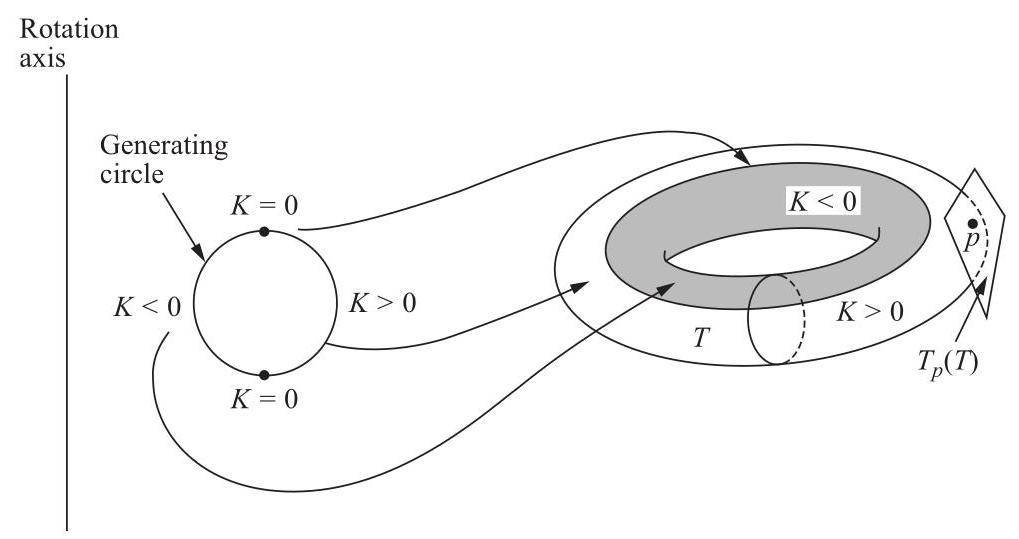
\includegraphics[max width=0.9\textwidth]{images/bo_d4b9jf3ef24c73e0334g_171_250_192_1019_539_0.jpg}
\end{center}
\hspace*{3em} 

图 3-15

命题 1. 令 \(\mathrm{p} \in  S\) 为曲面 \(S\) 的一个椭圆点.则存在 \(S\) 中 \(\mathrm{p}\) 的一个邻域 \(\mathrm{V}\) ，使得 \(\mathrm{V}\) 中的所有点都位于切平面 \({\mathrm{T}}_{\mathrm{p}}\left( S\right)\) 的同一侧.令 \(\mathrm{p} \in  S\) 为一个双曲点.则在 \(\mathrm{p}\) 的每个邻域中都存在 \(S\) 中位于 \({\mathrm{T}}_{\mathrm{p}}\left( S\right)\) 两侧的点.

证明.令 \(\mathbf{x}\left( {u,v}\right)\) 为 \(p\) 中的一个参数化，其中 \(\mathbf{x}\left( {0,0}\right)  = p\) .点 \(q = \mathbf{x}\left( {u,v}\right)\) 到切平面 \({T}_{p}\left( S\right)\) 的距离 \(d\) 由下式给出(图 3-16)

\[
d = \langle \mathbf{x}\left( {u,v}\right)  - \mathbf{x}\left( {0,0}\right) ,N\left( p\right) \rangle .
\]

因为 \(\mathbf{x}\left( {u,v}\right)\) 是可微的，我们有泰勒公式:

\[
\mathbf{x}\left( {u,v}\right)  = \mathbf{x}\left( {0,0}\right)  + {\mathbf{x}}_{u}u + {\mathbf{x}}_{v}v + \frac{1}{2}\left( {{\mathbf{x}}_{uu}{u}^{2} + 2{\mathbf{x}}_{uv}{uv} + {\mathbf{x}}_{vv}{v}^{2}}\right)  + \bar{R},
\]

其中导数在 \(\left( {0,0}\right)\) 处取值，余项 \(\bar{R}\) 满足条件

\[
\mathop{\lim }\limits_{{\left( {u,v}\right)  \rightarrow  \left( {0,0}\right) }}\frac{\bar{R}}{{u}^{2} + {v}^{2}} = 0.
\]

由此得出

\[
d = \langle \mathbf{x}\left( {u,v}\right)  - \mathbf{x}\left( {0,0}\right) ,N\left( p\right) \rangle
\]

\[
= \frac{1}{2}\left\{  {{\mathbf{x}}_{uu},N\left( p\right) {u}^{2} + 2\left\langle  {{\mathbf{x}}_{uv},N\left( p\right) }\right\rangle  {uv} + \left\langle  {{\mathbf{x}}_{vv},N\left( p\right) }\right\rangle  {v}^{2}}\right\}   + R
\]

\[
= \frac{1}{2}\left( {e{u}^{2} + {2fuv} + g{v}^{2}}\right)  + R = \frac{1}{2}{\Pi }_{p}\left( w\right)  + R,
\]

\begin{center}
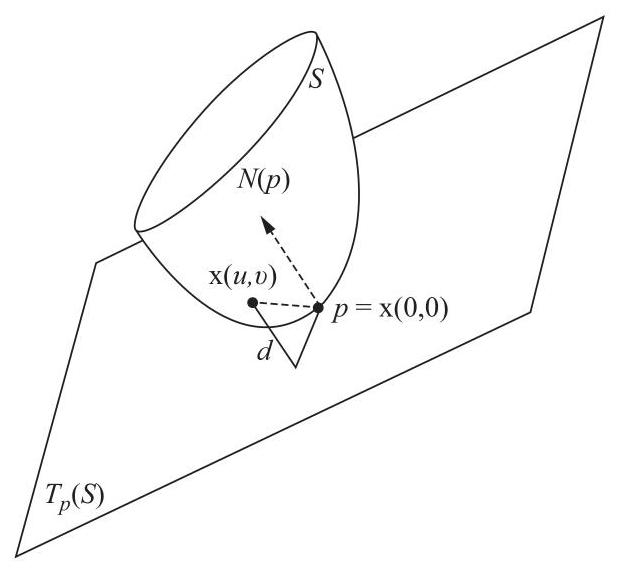
\includegraphics[max width=0.5\textwidth]{images/bo_d4b9jf3ef24c73e0334g_172_198_190_617_575_0.jpg}
\end{center}
\hspace*{3em} 

图 3-16

其中 \(w = {\mathbf{x}}_{u}u + {\mathbf{x}}_{v}v,R = \langle \bar{R},N\left( p\right) \rangle\) ，以及 \(\mathop{\lim }\limits_{{w \rightarrow  0}}\left( {R/{\left| w\right| }^{2}}\right)  = 0\) .

对于一个椭圆点 \(p,{\Pi }_{p}\left( w\right)\) 具有固定的符号.因此，对于所有 \(\left( {u,v}\right)\) 足够接近 \(p,d\) 的点，其符号与 \(I{I}_{p}\left( w\right)\) 相同；也就是说，所有这样的 \(\left( {u,v}\right)\) 都属于 \({T}_{p}\left( S\right)\) 的同一侧.

对于一个双曲点 \(p\) ，在 \(p\) 的每个邻域中都存在点 \(\left( {u,v}\right)\) 和 \(\left( {\bar{u},\bar{v}}\right)\) ，使得 \({\Pi }_{p}\left( {w/\left| w\right| }\right)\) 和 \({\Pi }_{p}\left( {\bar{w}/\left| \bar{w}\right| }\right)\) 具有相反的符号(此处 \(\bar{w} = {\mathbf{x}}_{u}\bar{u} + {\mathbf{x}}_{v}\bar{v}\) )；因此，这些点属于 \({T}_{p}\left( S\right)\) 的不同侧.Q.E.D.

在抛物点或平面点的邻域中，无法做出类似命题 1 的陈述.在上述抛物点和平面点的例子中(参见第 3-2 节的示例 3 和 6)，曲面位于切平面的同一侧，并可能与该平面共有一条直线.在接下来的例子中，我们将展示可能出现完全不同的情况.

示例 2.“猴子鞍”(参见图 3-17)由下式给出

\[
x = u,\;y = v,\;z = {u}^{3} - 3{v}^{2}u.
\]

直接计算表明，在 \(\left( {0,0}\right)\) 处，二次基本形式的系数为 \(e = f = g = 0\) ；因此，点 \(\left( {0,0}\right)\) 是一个平面点.然而，在该点的任何邻域中，都存在位于其切平面两侧的点.

\begin{center}
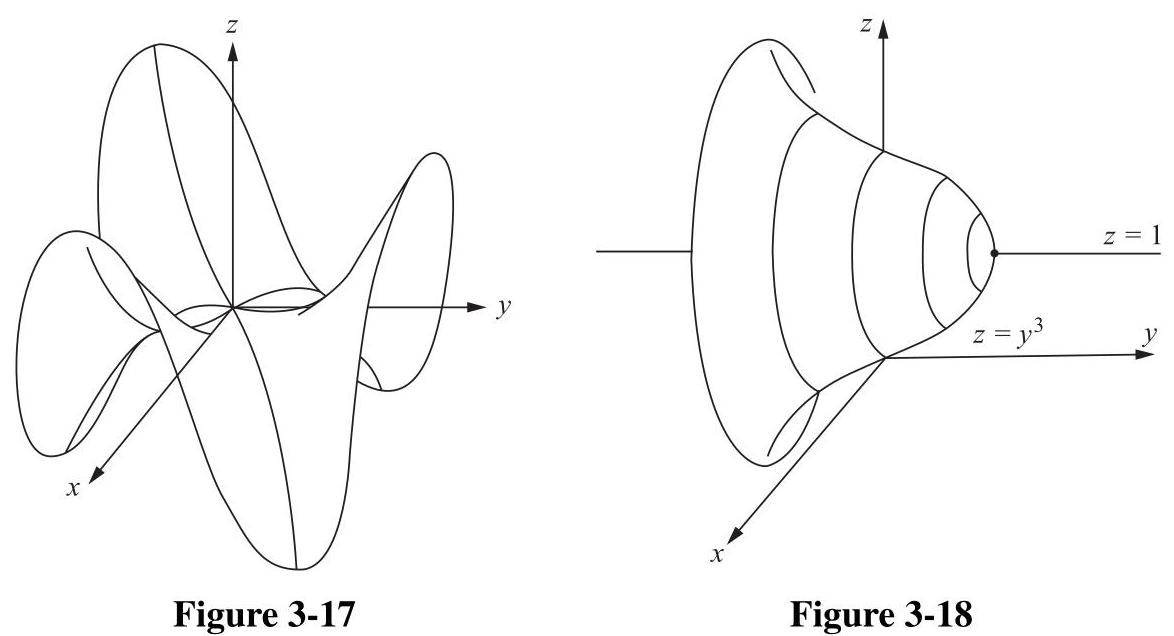
\includegraphics[max width=1.0\textwidth]{images/bo_d4b9jf3ef24c73e0334g_173_173_196_1174_636_0.jpg}
\end{center}
\hspace*{3em} 

示例 3.考虑通过将曲线 \(z = {y}^{3}\) ， \(- 1 < z < 1\) 绕直线 \(z = 1\) 旋转得到的曲面(参见图 3-18).简单的计算表明，由原点 \(O\) 的旋转产生的点是抛物点.我们将省略此计算，因为我们很快将证明(示例 4)旋转曲面的平行线和经线是曲率线；这，连同所讨论的点，经线(形式为 \(y = {x}^{3}\) 的曲线)的曲率为零，而平行线是法截线，将意味着上述陈述.

请注意，在这样的抛物点的任何邻域中，都存在位于切平面两侧的点.

二次基本形式在局部坐标中的表达式对于研究渐近方向和主方向特别有用.我们首先看渐近方向.

设 \(\mathbf{x}\left( {u,v}\right)\) 是在 \(p \in  S\) 处的一个参数化，其中 \(\mathbf{x}\left( {0,0}\right)  = p\) ，并且设 \(e\left( {u,v}\right)  = e,f\left( {u,v}\right)  = f\) 和 \(g\left( {u,v}\right)  = g\) 是该参数化中二次基本形式的系数.

我们回顾一下(参见 3-2 节定义 9)在 \(\mathbf{x}\) 的坐标邻域中的连通正则曲线 \(C\) 是渐近曲线，当且仅当对于 \(C\) 的任何参数化 \(\alpha \left( t\right)  = \mathbf{x}\left( {u\left( t\right) ,v\left( t\right) }\right) ,t \in  I\) ，我们有 \({II}\left( {{\alpha }^{\prime }\left( t\right) }\right)  = 0\) ，对于所有 \(t \in  I\) ，即当且仅当

\[
e{\left( {u}^{\prime }\right) }^{2} + {2f}{u}^{\prime }{v}^{\prime } + g{\left( {v}^{\prime }\right) }^{2} = 0,\;t \in  I. \tag{7}
\]

因此，式 (7) 被称为渐近曲线的微分方程.在下一节中，我们将为此表达式赋予更精确的含义.目前，我们只想从式 (7) 中得出以下有用的结论:一个双曲点 \(\left( {\mathrm{{eg}} - {\mathrm{f}}^{2} < 0}\right)\) 的邻域中的参数化使得参数化的坐标曲线是渐近曲线的充要条件是 \(\mathrm{e} = \mathrm{g} = 0.\)

事实上，如果两条曲线 \(u =\) const., \(v = v\left( t\right)\) 和 \(u = u\left( t\right) ,v =\) const. 都满足式 (7)，我们得到 \(e = g = 0\) .反之，如果最后一个条件成立且 \(f \neq  0\) ，式 (7) 变为 \(f{u}^{\prime }{v}^{\prime } = 0\) ，这显然被坐标线满足.

现在我们将考虑主方向，并保持已建立的符号.

坐标邻域 \(\mathbf{x}\) 中的连通正则曲线 \(C\) 是曲率线当且仅当对于 \(C\) 的任意参数化 \(\alpha \left( t\right)  = \mathbf{x}\left( {u\left( t\right) ,v\left( t\right) }\right)\) ，有(参见 3-2 节命题 3) \(t \in  I\)

\[
{dN}\left( {{\alpha }^{\prime }\left( t\right) }\right)  = \lambda \left( t\right) {\alpha }^{\prime }\left( t\right) .
\]

由此可知，函数 \({u}^{\prime }\left( t\right) ,{v}^{\prime }\left( t\right)\) 满足方程组

\[
\frac{{fF} - {eG}}{{EG} - {F}^{2}}{u}^{\prime } + \frac{{gF} - {fG}}{{EG} - {F}^{2}}{v}^{\prime } = \lambda {u}^{\prime },
\]

\[
\frac{{eF} - {fE}}{{EG} - {F}^{2}}{u}^{\prime } + \frac{{fF} - {gE}}{{EG} - {F}^{2}}{v}^{\prime } = \lambda {v}^{\prime }.
\]

通过消去上述方程组中的 \(\lambda\) ，我们得到曲率线的微分方程，

\[
\left( {{fE} - {eF}}\right) {\left( {u}^{\prime }\right) }^{2} + \left( {{gE} - {eG}}\right) {u}^{\prime }{v}^{\prime } + \left( {{gF} - {fG}}\right) {\left( {v}^{\prime }\right) }^{2} = 0,
\]

可以更对称地写成

\[
\left| \begin{matrix} {\left( {v}^{\prime }\right) }^{2} &  - {u}^{\prime }{v}^{\prime } & {\left( {u}^{\prime }\right) }^{2} \\  E & F & G \\  e & f & g \end{matrix}\right|  = 0. \tag{8}
\]

利用主方向相互正交的事实，从式 (8) 可以很容易地得出，参数化的坐标曲线在非脐点邻域中是曲率线的充要条件是 \(F = f = 0\) .

例 4(旋转曲面).考虑一个旋转曲面，其参数化为(参见 2-3 节例 4；我们已将 \(f\) 和 \(g\) 分别替换为 \(\varphi\) 和 \(\psi\) )

\[
\mathbf{x}\left( {u,v}\right)  = \left( {\varphi \left( v\right) \cos u,\varphi \left( v\right) \sin u,\psi \left( v\right) }\right) ,
\]

\[
0 < u < {2\pi },\;a < v < b,\;\varphi \left( v\right)  \neq  0.
\]

第一基本形式的系数由下式给出

\[
E = {\varphi }^{2},\;F = 0,\;G = {\left( {\varphi }^{\prime }\right) }^{2} + {\left( {\psi }^{\prime }\right) }^{2}.
\]

我们方便地假设旋转曲线是通过弧长参数化的，即

\[
{\left( {\varphi }^{\prime }\right) }^{2} + {\left( {\psi }^{\prime }\right) }^{2} = G = 1.
\]

第二基本形式系数的计算很简单，得到

\[
e = \frac{\left( {\mathbf{x}}_{u},{\mathbf{x}}_{v},{\mathbf{x}}_{uu}\right) }{\sqrt{{EG} - {F}^{2}}} = \frac{1}{\sqrt{{EG} - {F}^{2}}}\left| \begin{matrix}  - \varphi \sin u & {\varphi }^{\prime }\cos u &  - \varphi \cos u \\  \varphi \cos u & {\varphi }^{\prime }\sin u &  - \varphi \sin u \\  0 & {\psi }^{\prime } & 0 \end{matrix}\right|
\]

\[
=  - \varphi {\psi }^{\prime }
\]

\[
f = 0,
\]

\[
g = {\psi }^{\prime }{\varphi }^{\prime \prime } - {\psi }^{\prime \prime }{\varphi }^{\prime }.
\]

由于 \(F = f = 0\) ，我们得出旋转曲面的平行线( \(v =\) const.)和经线 \(\left( {u = \text{ const. }}\right)\) 是该曲面的曲率线(这一点在例 3 中已使用).

因为

\[
K = \frac{{eg} - {f}^{2}}{{EG} - {F}^{2}} =  - \frac{{\psi }^{\prime }\left( {{\psi }^{\prime }{\varphi }^{\prime \prime } - {\psi }^{\prime \prime }{\varphi }^{\prime }}\right) }{\varphi }
\]

且 \(\varphi\) 总是正的，所以抛物点由 \({\psi }^{\prime } = 0\) (生成曲线的切线垂直于旋转轴)或 \({\varphi }^{\prime }{\psi }^{\prime \prime } - {\psi }^{\prime }{\varphi }^{\prime \prime } = 0\) (生成曲线的曲率为零)给出.满足这两个条件的点是平面点，因为这些条件意味着 \(e = f = g = 0\) .

将高斯曲率写成另一种形式是方便的.通过微分 \({\left( {\varphi }^{\prime }\right) }^{2} + {\left( {\psi }^{\prime }\right) }^{2} = 1\) ，我们得到 \({\varphi }^{\prime }{\varphi }^{\prime \prime } =  - {\psi }^{\prime }{\psi }^{\prime \prime }\) .因此，

\[
K =  - \frac{{\psi }^{\prime }\left( {{\psi }^{\prime }{\varphi }^{\prime \prime } - {\psi }^{\prime \prime }{\varphi }^{\prime }}\right) }{\varphi } =  - \frac{{\left( {\psi }^{\prime }\right) }^{2}{\varphi }^{\prime \prime } + {\left( {\varphi }^{\prime }\right) }^{2}{\varphi }^{\prime \prime }}{\varphi } =  - \frac{{\varphi }^{\prime \prime }}{\varphi }. \tag{9}
\]

方程 (9) 是旋转曲面高斯曲率的方便表达式.例如，它可用于确定具有恒定高斯曲率的旋转曲面(参见练习 7).

为了计算主曲率，我们首先进行以下一般观察:如果正则曲面的参数化使得 \(F = f = 0\) ，则主曲率由 \(e/E\) 和 \(g/G\) 给出.事实上，在这种情况下，高斯曲率和平均曲率由(参见方程 (4) 和 (5))给出

\[
K = \frac{eg}{EG},\;H = \frac{1}{2}\frac{{eG} + {gE}}{EG}.
\]

由于 \(K\) 是主曲率的乘积，而 \({2H}\) 是主曲率的和，因此我们的论断立即成立.

因此，旋转曲面的主曲率由下式给出

\[
\frac{e}{E} =  - \frac{{\psi }^{\prime }\varphi }{{\varphi }^{2}} =  - \frac{{\psi }^{\prime }}{\varphi },\;\frac{g}{G} = {\psi }^{\prime }{\varphi }^{\prime \prime } - {\psi }^{\prime \prime }{\varphi }^{\prime }; \tag{10}
\]

因此，该曲面的平均曲率为

\[
H = \frac{1}{2}\frac{-{\psi }^{\prime } + \varphi \left( {{\psi }^{\prime }{\varphi }^{\prime \prime } - {\psi }^{\prime \prime }{\varphi }^{\prime }}\right) }{\varphi }. \tag{11}
\]

例 5. 很多时候，曲面被表示为可微函数(参见命题 1，第 2-2 节) \(z = h\left( {x,y}\right)\) 的图像，其中 \(\left( {x,y}\right)\) 属于开集 \(U \subset  {R}^{2}\) .因此，在这种情况下，拥有相关概念的公式是很方便的.为了得到这样的公式，让我们用以下方式对曲面进行参数化:

\[
\mathbf{x}\left( {u,v}\right)  = \left( {u,v,h\left( {u,v}\right) }\right) ,\;\left( {u,v}\right)  \in  U,
\]

其中 \(u = x,v = y\) .简单的计算表明

\[
{\mathbf{x}}_{u} = \left( {1,0,{h}_{u}}\right) ,\;{\mathbf{x}}_{v} = \left( {0,1,{h}_{v}}\right) ,\;{\mathbf{x}}_{uu} = \left( {0,0,{h}_{uu}}\right) ,
\]

\[
{\mathbf{x}}_{uv} = \left( {0,0,{h}_{uu}}\right) ,\;{\mathbf{x}}_{vv} = \left( {0,0,{h}_{vv}}\right) .
\]

因此

\[
N\left( {x,y}\right)  = \frac{\left( -{h}_{x}, - {h}_{y},1\right) }{{\left( 1 + {h}_{x}^{2} + {h}_{y}^{2}\right) }^{1/2}}
\]

是曲面上的单位法向量场，并且在此方向下的第二基本形式的系数由下式给出

\[
e = \frac{{h}_{xx}}{{\left( 1 + {h}_{x}^{2} + {h}_{y}^{2}\right) }^{1/2}},
\]

\[
f = \frac{{h}_{xy}}{{\left( 1 + {h}_{x}^{2} + {h}_{y}^{2}\right) }^{1/2}},
\]

\[
g = \frac{{h}_{yy}}{{\left( 1 + {h}_{x}^{2} + {h}_{y}^{2}\right) }^{1/2}}.
\]

从上述表达式，可以轻松计算出任何所需的公式.例如，从方程 (4) 和 (5) 中，我们得到高斯曲率和平均曲率:

\[
K = \frac{{h}_{xx}{h}_{yy} - {h}_{xy}^{2}}{{\left( 1 + {h}_{x}^{2} + {h}_{y}^{2}\right) }^{2}},
\]

\[
{2H} = \frac{\left( {1 + {h}_{x}^{2}}\right) {h}_{yy} - 2{h}_{x}{h}_{y}{h}_{xy} + \left( {1 + {h}_{y}^{2}}\right) {h}_{xx}}{{\left( 1 + {h}_{x}^{2} + {h}_{y}^{2}\right) }^{3/2}}.
\]

研究由 \(z = h\left( {x,y}\right)\) 给出的曲面还有另一个，也许更重要的原因.这是因为在局部上，任何曲面都是可微函数(参见命题 3，第 2-2 节)的图像.给定曲面 \(S\) 的一个点 \(p\) ，我们可以选择 \({R}^{3}\) 的坐标轴，使得坐标的原点 \(O\) 位于 \(p\) 处，并且 \(z\) 轴沿着 \(S\) 在 \(p\) 处的正法线方向(因此， \({xy}\) 平面与 \({T}_{p}\left( S\right)\) 一致).由此可知， \(S\) 中 \(p\) 的一个邻域可以表示为 \(z = h\left( {x,y}\right) ,\left( {x,y}\right)  \in  U \subset  {R}^{2}\) 的形式，其中 \(U\) 是一个开集， \(h\) 是一个可微函数(参见命题 3，第 2-2 节)，且 \(h\left( {0,0}\right)  = 0,{h}_{x}\left( {0,0}\right)  = 0,{h}_{y}\left( {0,0}\right)  = 0\) (图 3-19).

\begin{center}
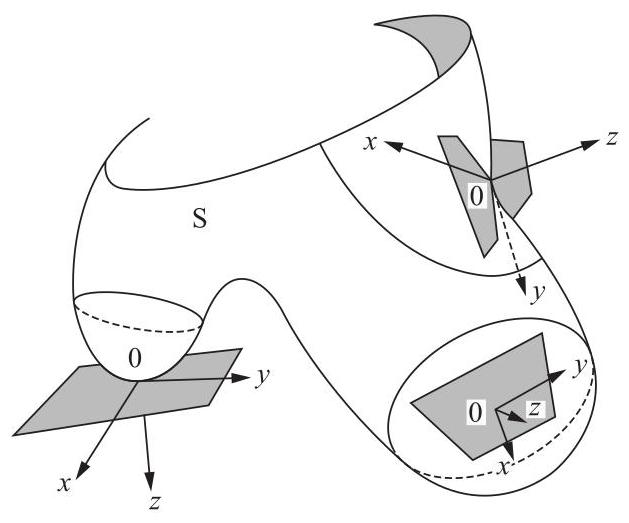
\includegraphics[max width=0.5\textwidth]{images/bo_d4b9jf3ef24c73e0334g_177_181_1071_629_523_0.jpg}
\end{center}
\hspace*{3em} 

图 3-19. \(S\) 的每个点都有一个可以写成 \(z = h\left( {x,y}\right)\) 的邻域.

在这种情况下， \(S\) 在 \(p\) 处的第二基本形式应用于向量 \(\left( {x,y}\right)  \in  {R}^{2}\) 变为:

\[
{h}_{xx}\left( {0,0}\right) {x}^{2} + 2{h}_{xy}\left( {0,0}\right) {xy} + {h}_{yy}\left( {0,0}\right) {y}^{2}.
\]

在二元微积分中，上述二次型被称为 \(h\) 在 \(\left( {0,0}\right)\) 处的 Hessian.因此， \(h\) 在 \(\left( {0,0}\right)\) 处的 Hessian 是 \(S\) 在 \(p\) 处的第二基本形式.

让我们应用上述考虑来给出 Dupin 示性曲面的几何解释.使用上述符号，设 \(\epsilon  > 0\) 是一个小的数，使得

\[
C = \left\{  {\left( {x,y}\right)  \in  {T}_{p}\left( S\right) ;h\left( {x,y}\right)  = \epsilon }\right\}
\]

是一条正则曲线(我们可能需要改变曲面的方向以实现 \(\epsilon  > 0\) ).我们想证明，如果 \(p\) 不是平面点，则曲线 \(C\) “近似”类似于 \(S\) 在 \(p\) 处的 Dupin 指示曲面(图 3-20).

\begin{center}
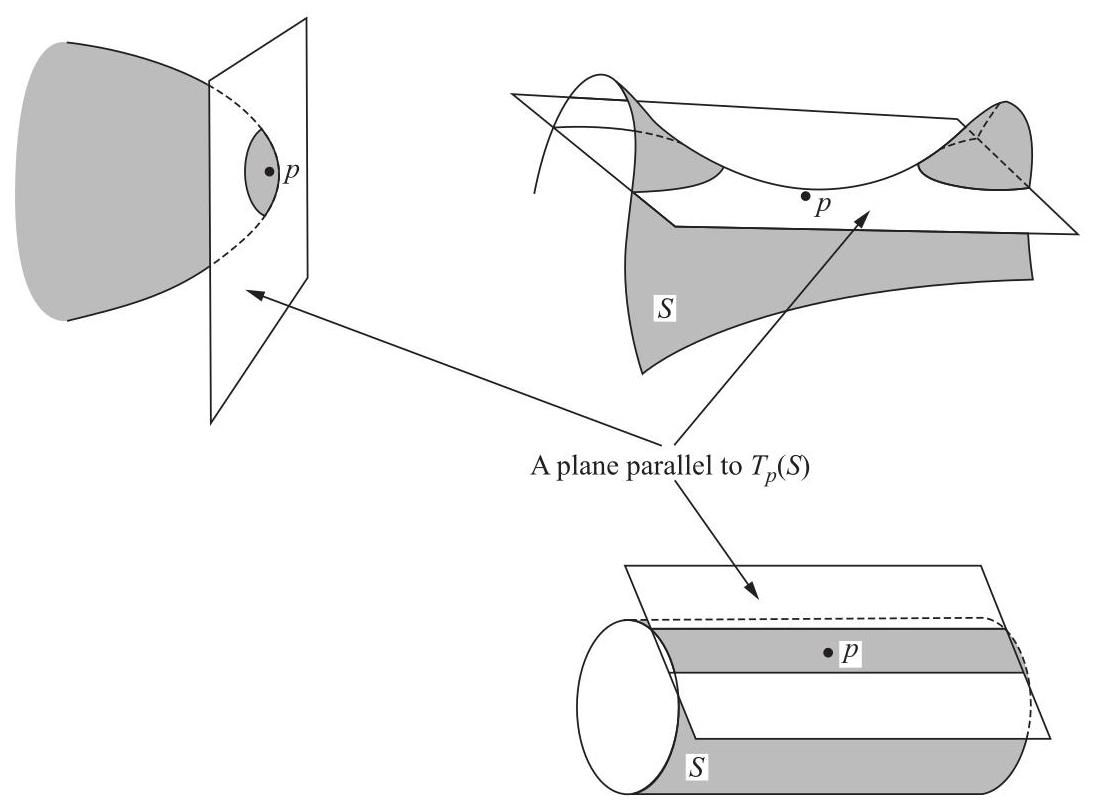
\includegraphics[max width=0.9\textwidth]{images/bo_d4b9jf3ef24c73e0334g_178_235_477_1093_806_0.jpg}
\end{center}
\hspace*{3em} 

图 3-20

为了说明这一点，我们进一步假设 \(x\) 和 \(y\) 轴沿主方向，其中 \(x\) 轴沿最大主曲率方向.因此， \(f = {h}_{xy}\left( {0,0}\right)  = 0\) 和

\[
{k}_{1}\left( p\right)  = \frac{e}{E} = {h}_{xx}\left( {0,0}\right) ,\;{k}_{2}\left( p\right)  = \frac{g}{G} = {h}_{yy}\left( {0,0}\right) .
\]

通过将 \(h\left( {x,y}\right)\) 关于 \(\left( {0,0}\right)\) 进行泰勒展开，并考虑到 \({h}_{x}\left( {0,0}\right)  = 0 = {h}_{y}\left( {0,0}\right)\) ，我们得到

\[
h\left( {x,y}\right)  = \frac{1}{2}\left( {{h}_{xx}\left( {0,0}\right) {x}^{2} + 2{h}_{xy}\left( {0,0}\right) {xy} + {h}_{yy}\left( {0,0}\right) {y}^{2}}\right)  + R
\]

\[
= \frac{1}{2}\left( {{k}_{1}{x}^{2} + {k}_{2}{y}^{2}}\right)  + R,
\]

其中

\[
\mathop{\lim }\limits_{{\left( {x,y}\right)  \rightarrow  \left( {0,0}\right) }}\frac{R}{{x}^{2} + {y}^{2}} = 0.
\]

因此，曲线 \(C\) 由下式给出

\[
{k}_{1}{x}^{2} + {k}_{2}{y}^{2} + {2R} = {2\epsilon }.
\]

现在，如果 \(p\) 不是平面点，我们可以将 \({k}_{1}{x}^{2} + {k}_{2}{y}^{2} = {2\epsilon }\) 视为 \(p\) 邻域中 \(C\) 的一阶近似.通过使用相似变换，

\[
x = \bar{x}\sqrt{2\epsilon },\;y = \bar{y}\sqrt{2\epsilon },
\]

我们得到 \({k}_{1}{x}^{2} + {k}_{2}{y}^{2} = {2\epsilon }\) 被变换为曲线

\[
{k}_{1}{\bar{x}}^{2} + {k}_{2}{\bar{y}}^{2} = 1,
\]

这是 \(p\) 处的 Dupin 指示曲面.这意味着，如果 \(\mathrm{p}\) 是非平面点，则与 \(\mathrm{p}\) 相近的平行于 \({\mathrm{T}}_{\mathrm{p}}\left( S\right)\) 的平面与 \(S\) 的交线，在一阶近似下，是一条与 p 处的 Dupin 指示曲面相似的曲线.

如果 \(p\) 是平面点，则此解释不再有效(参见练习 11).

为了结束本节，我们将给出高斯曲率在高斯映射 \(N : S \rightarrow  {S}^{2}\) 方面的几何解释.实际上，高斯本人就是这样引入这个曲率的.

为此，我们首先需要一个定义.

设 \(S\) 和 \(\bar{S}\) 为两个定向正则曲面.设 \(\varphi  : S \rightarrow  \bar{S}\) 为一个可微映射，并假设对于某个 \(p \in  S,d{\varphi }_{p}\) 是非奇异的.如果给定 \({T}_{p}\left( S\right)\) 中的一个正基 \(\left\{  {{w}_{1},{w}_{2}}\right\}\) ，则 \({T}_{\varphi \left( p\right) }\left( \bar{S}\right)\) 中的 \(\left\{  {d{\varphi }_{p}\left( {w}_{1}\right) ,d{\varphi }_{p}\left( {w}_{2}\right) }\right\}\) 是一个正基，我们称 \(\varphi\) 在 \(p\) 处是保持方向的.如果 \(\left\{  {d{\varphi }_{p}\left( {w}_{1}\right) ,d{\varphi }_{p}\left( {w}_{2}\right) }\right\}\) 不是正基，我们称 \(\varphi\) 在 \(p\) 处是反转方向的.

我们现在观察到 \(S\) 和单位球面 \({S}^{2}\) 都嵌入在 \({R}^{3}\) 中.因此， \(S\) 上的一个方向 \(N\) 在 \({S}^{2}\) 中诱导一个方向 \(N\) .设 \(p \in  S\) 使得 \(d{N}_{p}\) 非奇异.因为对于 \({T}_{p}\left( S\right)\) 中的基 \(\left\{  {{w}_{1},{w}_{2}}\right\}\)

\[
d{N}_{p}\left( {w}_{1}\right)  \land  d{N}_{p}\left( {w}_{2}\right)  = \det \left( {d{N}_{p}}\right) \left( {{w}_{1} \land  {w}_{2}}\right)  = K{w}_{1} \land  {w}_{2},
\]

高斯映射 \(N\) 在 \(p \in  S\) 处是保向的，如果 \(K\left( p\right)  > 0\) ；在高斯映射 \(N\) 在 \(p \in  S\) 处是反向的，如果 \(K\left( p\right)  < 0\) .直观地说，这意味着(图 3-21): \({T}_{p}\left( S\right)\) 的一个定向诱导了 \(S\) 中围绕 \(p\) 的小闭曲线的定向；这些曲线经过 \(N\) 的像的定向与初始定向相同或相反，取决于 \(p\) 分别是椭圆点还是双曲点.

为了将这一事实考虑在内，我们约定，区域 \(N\) 的图像面积为连通邻域 \(V \subset  S\) 中的一个区域，其中 \(K \neq  0\) 如果 \(K > 0\) 则为正，如果 \(K < 0\) 则为负(因为 \(V\) 是连通的， \(K\) 在 \(V\) 中符号不变).

现在我们可以给出高斯曲率 \(K\) 对 \(K \neq  0\) 的承诺的几何解释了.

\begin{center}
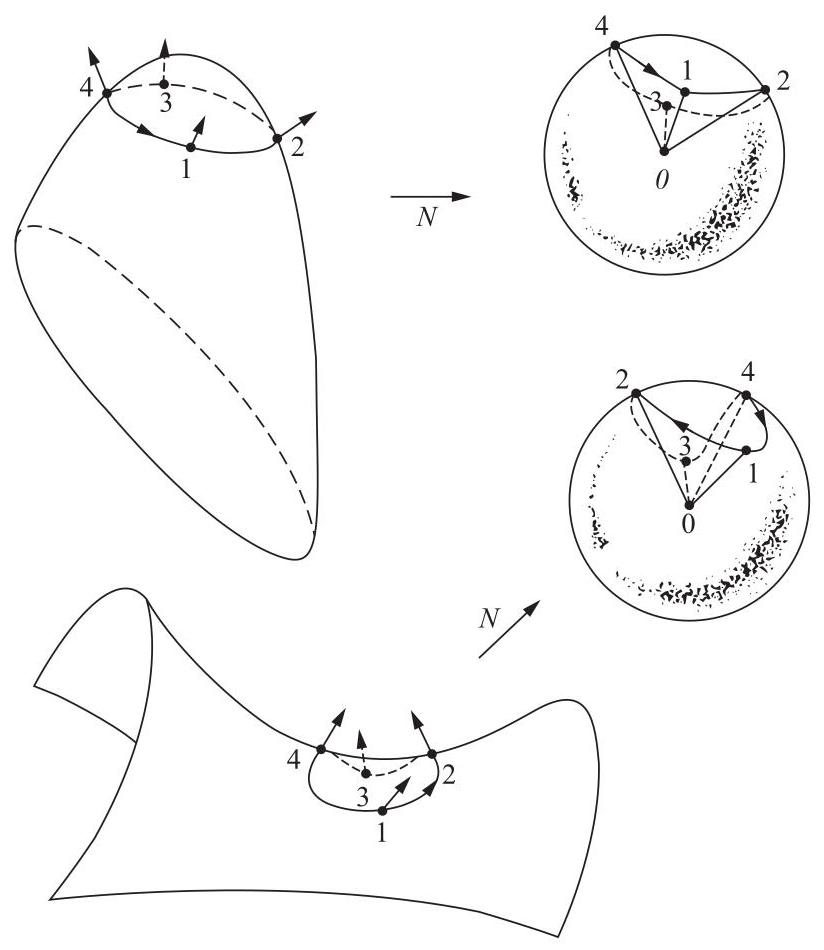
\includegraphics[max width=0.7\textwidth]{images/bo_d4b9jf3ef24c73e0334g_180_371_193_824_950_0.jpg}
\end{center}
\hspace*{3em} 

图 3-21.高斯映射在椭圆点处保持定向，在双曲点处反转定向.

命题 2. 令 \(\mathrm{p}\) 为曲面 \(S\) 上一点，其高斯曲率为 \(\mathrm{K}\left( \mathrm{p}\right)  \neq  0\) ，令 \(\mathrm{V}\) 为 \(\mathrm{p}\) 的一个连通邻域，其中 \(\mathrm{K}\) 不改变符号.则

\[
\mathrm{K}\left( \mathrm{p}\right)  = \mathop{\lim }\limits_{{\mathrm{A} \rightarrow  0}}\frac{{\mathrm{A}}^{\prime }}{\mathrm{A}}
\]

其中 \(\mathrm{A}\) 是区域 \(\mathrm{B} \subset  \mathrm{V}\) 的面积，该区域包含 \(\mathrm{p},{\mathrm{A}}^{\prime }\) 是区域 \(\mathrm{B}\) 经过高斯映射 \(N : S \rightarrow  {S}^{2}\) 的像的面积，并且极限是通过一个区域序列 \({\mathrm{B}}_{N}\) 取的，该序列收敛于 \(\mathrm{p}\) ，其意义是，围绕 \(\mathrm{p}\) 的任何球体都包含所有 \({\mathrm{B}}_{N}\) ，对于足够大的 \(N\) .

证明.区域 \(B\) 的面积 \(A\) 由下式给出(参见第 2-5 节)

\[
A = {\iint }_{R}\left| {{\mathbf{x}}_{u} \land  {\mathbf{x}}_{v}}\right| {dudv}
\]

其中 \(\mathbf{x}\left( {u,v}\right)\) 是 \(p\) 中的一个参数化，其坐标邻域包含 \(V\) (可以假设 \(V\) 足够小)， \(R\) 是 \({uv}\) 平面中对应于 \(B\) 的区域.区域 \(N\left( B\right)\) 的面积 \({A}^{\prime }\) 为

\[
{A}^{\prime } = {\iint }_{R}\left| {{N}_{u} \land  {N}_{v}}\right| {dudv}
\]

使用公式 (1)、 \(K\) 的定义以及上述约定，我们可以写出

\[
{A}^{\prime } = {\iint }_{R}K\left| {{\mathbf{x}}_{u} \land  {\mathbf{x}}_{v}}\right| {dudv} \tag{12}
\]

取极限，并同样用 \(R\) 表示区域 \(R\) 的面积，我们得到

\[
\mathop{\lim }\limits_{{A \rightarrow  0}}\frac{{A}^{\prime }}{A} = \mathop{\lim }\limits_{{R \rightarrow  0}}\frac{{A}^{\prime }/R}{A/R} = \frac{\mathop{\lim }\limits_{{R \rightarrow  0}}\left( {1/R}\right) {\iint }_{R}K\left| {{\mathbf{x}}_{u} \land  {\mathbf{x}}_{v}}\right| {dudv}}{\mathop{\lim }\limits_{{R \rightarrow  0}}\left( {1/R}\right) {\iint }_{R}\left| {{\mathbf{x}}_{u} \land  {\mathbf{x}}_{v}}\right| {dudv}}
\]

\[
= \frac{K\left| {{\mathbf{x}}_{u} \land  {\mathbf{x}}_{v}}\right| }{\left| {\mathbf{x}}_{u} \land  {\mathbf{x}}_{v}\right| } = K
\]

(注意到我们使用了双重积分的均值定理)，这就证明了该命题.证毕.

备注.将命题与曲率的表达式进行比较

\[
k = \mathop{\lim }\limits_{{s \rightarrow  0}}\frac{\sigma }{s}
\]

(此处 \(s\) 是包含 \(p\) 的 \(C\) 的一小段弧长， \(\sigma\) 是其在切线指示图中的像的弧长；参见第 1-5 节的练习 3)，我们看到高斯曲率 \(K\) 是曲面上的类比，对应于平面曲线的曲率 \(k\) .

\exerciseline

1. 证明在双曲面 \(z = {axy}\) 的原点 \(\left( {0,0,0}\right)\) 处，我们有 \(K =  - {a}^{2}\) 和 \(H = 0\) .

*2. 确定螺旋面 \(x = v\cos u,y = v\sin u,z = {cu}\) 的渐近线和曲率线，并证明其平均曲率为零.

*3. 确定悬链面

\[
\mathbf{x}\left( {u,v}\right)  = \left( {\cosh v\cos u,\cosh v\sin u,v}\right) .
\]

4. 确定 \(z = {xy}\) 的渐近线和曲率线.

5. 考虑参数化曲面(Enneper 曲面)

\[
\mathbf{x}\left( {u,v}\right)  = \left( {u - \frac{{u}^{3}}{3} + u{v}^{2},v - \frac{{v}^{3}}{3} + v{u}^{2},{u}^{2} - {v}^{2}}\right)
\]

并证明

a. 第一基本形式的系数是

\[
E = G = {\left( 1 + {u}^{2} + {v}^{2}\right) }^{2},\;F = 0.
\]

b. 第二基本形式的系数是

\[
e = 2,\;g =  - 2,\;f = 0.
\]

c. 主曲率是

\[
{k}_{1} = \frac{2}{{\left( 1 + {u}^{2} + {v}^{2}\right) }^{2}},\;{k}_{2} =  - \frac{2}{{\left( 1 + {u}^{2} + {v}^{2}\right) }^{2}}.
\]

d. 曲率线是坐标曲线.

e. 渐近线是 \(u + v =\) 为常数， \(u - v =\) 为常数.

6. (一个具有 \(K \equiv   - 1\) 的曲面；伪球面.)

a. 求平面曲线 \(C\) 的方程，该曲线的性质是:切线段在切点与平面上某条不与曲线相交的直线 \(r\) 之间，其长度恒等于 1(该曲线称为悬链线；见图 1-9).

b. 将悬链线 \(C\) 绕直线 \(r\) 旋转；确定由此得到的“旋转曲面”(伪球面；见图 3-22)是否规则，并求出规则点邻域的参数化.

c. 证明伪球面上任意规则点的Гаусс曲率恒为 -1.

7.(常曲率旋转曲面.)给定旋转曲面 \((\varphi \left( v\right) \cos u\) , \(\varphi \left( v\right) \sin u,\psi \left( v\right) ),\varphi  \neq  0\) 具有常 Гаусс曲率 \(K\) .为确定函数 \(\varphi\) 和 \(\psi\) ，选择参数 \(v\) 使得 \({\left( {\varphi }^{\prime }\right) }^{2} + {\left( {\psi }^{\prime }\right) }^{2} = 1\) (几何上，这意味着 \(v\) 是生成曲线 \(\left( {\varphi \left( v\right) ,\psi \left( v\right) }\right) )\) 的弧长.证明:

a. \(\varphi\) 满足 \({\varphi }^{\prime \prime } + {K\varphi } = 0\) 且 \(\psi\) 由 \(\psi  = \int \sqrt{1 - {\left( {\varphi }^{\prime }\right) }^{2}}{dv}\) 给出；因此， \(0 < u < {2\pi }\) ，且 \(v\) 的定义域使得最后一个积分有意义.

b. 所有与平面 \({xOy}\) 垂直相交的常曲率旋转曲面 \(K = 1\) 由下式给出:

\[
\varphi \left( v\right)  = C\cos v,\;\psi \left( v\right)  = {\int }_{0}^{v}\sqrt{1 - {C}^{2}{\sin }^{2}v}{dv},
\]

其中 \(C\) 是常数 \(\left( {C = \varphi \left( 0\right) }\right)\) .确定 \(v\) 的定义域，并绘制 \(C = 1,C > 1,C < 1\) 情况下的 \({xz}\) 平面上曲面轮廓的粗略草图.注意 \(C = 1\) 给出了一个球面(图 3-23).

\begin{center}
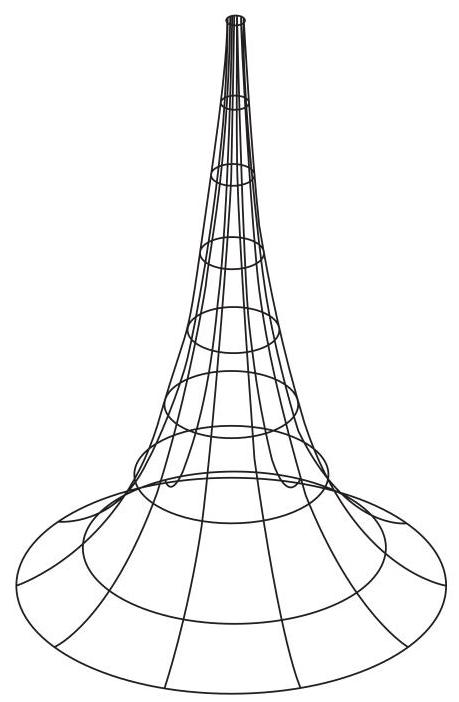
\includegraphics[max width=0.4\textwidth]{images/bo_d4b9jf3ef24c73e0334g_183_202_191_459_702_0.jpg}
\end{center}
\hspace*{3em} 

图 3-22. 伪球面.

\begin{center}
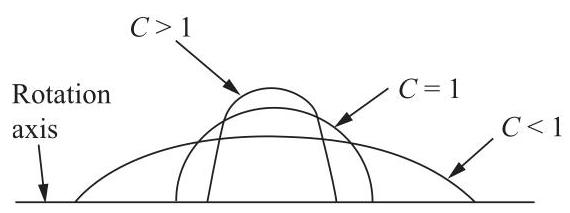
\includegraphics[max width=0.5\textwidth]{images/bo_d4b9jf3ef24c73e0334g_183_772_682_570_213_0.jpg}
\end{center}
\hspace*{3em} 

图 3-23

c. 所有常曲率旋转曲面 \(K =  - 1\) 可由以下类型之一给出:

1. \(\varphi \left( v\right)  = C\cosh v\) ,

\[
\psi \left( v\right)  = {\int }_{0}^{v}\sqrt{1 - {C}^{2}{\sinh }^{2}v}{dv}.
\]

2. \(\varphi \left( v\right)  = C\sinh v\) ,

\[
\psi \left( v\right)  = {\int }_{0}^{v}\sqrt{1 - {C}^{2}{\cosh }^{2}v}{dv}.
\]

3. \(\varphi \left( v\right)  = {e}^{v}\) ,

\(\psi \left( v\right)  = {\int }_{0}^{v}\sqrt{1 - {e}^{2v}}{dv}.\)

确定 \(v\) 的定义域，并绘制 \({xz}\) 平面上曲面轮廓的粗略草图.

d. 第 \(c\) 部分的类型 3 曲面是练习 6 中的伪球面.

e. 具有 \(K \equiv  0\) 的唯一旋转曲面是直圆柱面、直圆锥面和平面.

8.(曲面的 \(\geq  2\) 阶接触.)两个曲面 \(S\) 和 \(\bar{S}\) ，在共同点 \(p\) 处，如果在 \(p\) 处存在 \(S\) 和 \(\bar{S}\) 的参数化 \(\mathbf{x}\left( {u,v}\right)\) 和 \(\overline{\mathbf{x}}\left( {u,v}\right)\) ，使得

\[
{\mathbf{x}}_{u} = {\overline{\mathbf{x}}}_{u},\;{\mathbf{x}}_{v} = {\overline{\mathbf{x}}}_{v},\;{\mathbf{x}}_{uu} = {\overline{\mathbf{x}}}_{uu},\;{\mathbf{x}}_{uv} = {\overline{\mathbf{x}}}_{uv},\;{\mathbf{x}}_{vv} = {\overline{\mathbf{x}}}_{vv}
\]

在 \(p\) 处.证明以下命题:

设 \(S\) 和 \(\bar{S}\) 在 \(p\) 中是 \(S\) 和 \(\bar{S}\) 的任意参数化，其阶数为 \(\geq  2\) ，在 \(p;\mathbf{x} : U \rightarrow  S\) 和 \(\overline{\mathbf{x}} : U \rightarrow \; \bar{S}\) 处；并且设 \(f : V \subset  {R}^{3} \rightarrow  R\) 是 \({R}^{3}\) 中 \(p\) 的邻域 \(V\) 中的一个可微函数.那么 \(f \circ  \overline{\mathbf{x}} : U \rightarrow  R\) 的 \(\leq  2\) 阶偏导数在 \({\overline{\mathbf{x}}}^{-1}\left( p\right)\) 中为零，当且仅当 \(f \circ  \mathbf{x} : U \rightarrow  R\) 的 \(\leq  2\) 阶偏导数在 \({\mathbf{x}}^{-1}\left( p\right)\) 中为零.

*b. 设 \(S\) 和 \(\bar{S}\) 在 \(p\) 处具有 \(\geq  2\) 阶接触.设 \(z = f\left( {x,y}\right)\) 和 \(z = \bar{f}\left( {x,y}\right)\) 分别是 \(S\) 和 \(\bar{S}\) 在 \(p\) 邻域中的方程，其中 \({xy}\) 平面是 \(p = \left( {0,0}\right)\) 处的公共切平面.则函数 \(f\left( {x,y}\right)  - \bar{f}\left( {x,y}\right)\) 在 \(\left( {0,0}\right)\) 处的所有 \(\leq  2\) 阶偏导数都等于零.

c. 设 \(p\) 是曲面 \(S \subset  {R}^{3}\) 中的一点.设 \({Oxyz}\) 是 \({R}^{3}\) 的一个笛卡尔坐标系，使得 \(O = p\) 和 \({xy}\) 平面是 \(S\) 在 \(p\) 处的切平面.证明抛物面

\[
z = \frac{1}{2}\left( {{x}^{2}{f}_{xx} + {2xy}{f}_{xy} + {y}^{2}{f}_{yy}}\right) ,
\]
 (*)

在 \(p = \left( {0,0}\right)\) 附近泰勒展开中忽略三阶及更高阶项得到的抛物面，在 \(p\) 处与 \(S\) 具有 \(\geq  2\) 阶接触(曲面 \(\left( *\right)\) 称为 \(S\) 在 \(p\) 处的密切抛物面).

*d. 如果一个抛物面(包括平面和抛物柱面的退化情况)在 \(p\) 处与曲面 \(S\) 具有 \(\geq  2\) 阶接触，则它是 \(S\) 在 \(p\) 处的密切抛物面.

e. 如果两个曲面在 \(p\) 处具有 \(\geq  2\) 阶接触，则 \(S\) 和 \(\bar{S}\) 在 \(p\) 处的密切抛物面重合.由此得出 \(S\) 和 \(\bar{S}\) 在 \(p\) 处的曲率和平均曲率相等.

f. 接触阶数 \(\geq  2\) 的概念对于 \({R}^{3}\) 的微分同胚是不变的；也就是说，如果 \(S\) 和 \(\bar{S}\) 在 \(p\) 处具有 \(\geq  2\) 阶接触，并且 \(\varphi  : {R}^{3} \rightarrow  {R}^{3}\) 是一个微分同胚，那么 \(\varphi \left( S\right)\) 和 \(\varphi \left( \bar{S}\right)\) 在 \(\varphi \left( p\right)\) 处具有 \(\geq  2\) 阶接触.

g. 如果 \(S\) 和 \(\bar{S}\) 在 \(p\) 处具有 \(\geq  2\) 阶接触，则

\[
\mathop{\lim }\limits_{{r \rightarrow  0}}\frac{d}{{r}^{2}} = 0
\]

其中 \(d\) 是曲面在垂直于 \({T}_{p}\left( S\right)  = {T}_{p}\left( \bar{S}\right)\) 的直线上截取的线段的长度，该直线距离 \(p\) 为 \(r\) .

9. (曲线的接触.) 定义 \({R}^{3}\) 中具有公共点 \(p\) 的正则曲线的 \(\geq  n\left( {n\text{ integer } \geq  1}\right)\) 阶接触，并证明

a. \(\geq  n\) 阶接触的概念对于微分同胚是不变的.

b. 两条曲线在 \(p\) 处具有 \(\geq  1\) 阶接触，当且仅当它们在 \(p\) 处相切.

10. (曲线与曲面的接触.) 一条曲线 \(C\) 和一个曲面 \(S\) ，它们有一个公共点 \(p\) ，在 \(p\) 处具有 \(\geq  n\left( {n\text{ integer } \geq  1}\right)\) 阶接触，如果存在一条通过 \(p\) 的曲线 \(\bar{C} \subset  S\) ，使得 \(C\) 和 \(\bar{C}\) 在 \(p\) 处具有 \(\geq  n\) 阶接触.证明

a. 如果 \(f\left( {x,y,z}\right)  = 0\) 是 \(S\) 中 \(p\) 的邻域的表示，而 \(\alpha \left( t\right)  = \left( {x\left( t\right) ,y\left( t\right) ,z\left( t\right) }\right)\) 是 \(p\) 中 \(C\) 的参数化，其中 \(\alpha \left( 0\right)  = p\) ，那么 \(C\) 和 \(S\) 具有 \(\geq  n\) 阶接触，当且仅当

\[
f\left( {x\left( 0\right) ,y\left( 0\right) ,z\left( 0\right) }\right)  = 0,\;\frac{df}{dt} = 0,\ldots ,\frac{{d}^{n}f}{d{t}^{n}} = 0,
\]

其中导数是针对 \(t = 0\) 计算的.

b. 如果一个平面在 \(p\) 处与曲线 \(C\) 具有 \(\geq  2\) 阶接触，那么这个平面是 \(C\) 在 \(p\) 处的密切平面.

c. 如果一个球面在 \(p\) 处与曲线 \(C\) 具有 \(\geq  3\) 阶接触，并且 \(\alpha \left( s\right)\) 是该曲线的弧长参数化，其中 \(\alpha \left( 0\right)  = p\) ，那么球心由下式给出

\[
\alpha \left( 0\right)  + \frac{1}{k}n + \frac{{k}^{\prime }}{{k}^{2}\tau }b
\]

这样的球面称为 \(C\) 在 \(p\) 处的密切球面.

11. 考虑示例 2 的猴鞍 \(S\) .使用 3-2 节的定义构造 \(p = \left( {0,0,0}\right)\) 处的 Dupin 指示曲面，并将其与通过 \(S\) 与平行于 \({T}_{p}\left( S\right)\) 且接近 \(p\) 的平面相交得到的曲线进行比较.为什么它们不“近似相似”(参见 3-3 节的示例 5)？回顾 3-3 节示例 5 的论证，并指出其失效之处.

12. 考虑参数化曲面

\[
\mathbf{x}\left( {u,v}\right)  = \left( {\sin u\cos v,\sin u\sin v,\cos u + \log \tan \frac{u}{2} + \varphi \left( v\right) }\right) ,
\]

其中 \(\varphi\) 是一个可微函数.证明

a. 常数曲线 \(v =\) 包含在通过 \(z\) 轴并与曲面成恒定角度 \(\theta\) 的平面中，该角度由下式给出

\[
\cos \theta  = \frac{{\varphi }^{\prime }}{\sqrt{1 + {\left( {\varphi }^{\prime }\right) }^{2}}}.
\]

由此得出常数曲线 \(v =\) 是曲面的曲率线.

b. 常数曲线 \(v =\) 的切线段的长度，由其切点和 \(z\) 轴确定，恒等于 1.由此得出常数曲线 \(v =\) 是牵引曲线(参见练习 6).

13. 令 \(F : {R}^{3} \rightarrow  {R}^{3}\) 为由 \(F\left( p\right)  = {cp}\) 定义的映射(一种相似性)， \(p \in  {R}^{3},c\) 为正常数.令 \(S \subset  {R}^{3}\) 为一个正则曲面，并设 \(F\left( S\right)  = \bar{S}\) .证明 \(\bar{S}\) 是一个正则曲面，并找出联系 \(S\) 的高斯曲率和平均曲率 \(K\) 和 \(H\) 与 \(\bar{S}\) 的高斯曲率和平均曲率 \(\bar{K}\) 和 \(\bar{H}\) 的公式.

14. 考虑由曲线 \(y = {x}^{3}, - 1 < x < 1\) 绕直线 \(x = 1\) 旋转而得到的曲面.证明由曲线的起点 \(\left( {0,0}\right)\) 旋转得到的点是曲面的平面点.

*15. 给出一个具有孤立抛物点 \(p\) 的曲面示例(即，在 \(p\) 的某个邻域内不包含其他抛物点).

*16. 证明一个紧致曲面(即，在 \({R}^{3}\) 中有界且闭合)具有椭圆点.

17. 为不可定向曲面定义高斯曲率.你能为不可定向曲面定义平均曲率吗？

18. 证明图 3-1 的莫比乌斯带可以参数化为

\[
\mathbf{x}\left( {u,v}\right)  = \left( {\left( {2 - v\sin \frac{u}{2}}\right) \sin u,\left( {2 - v\sin \frac{u}{2}}\right) \cos u,v\cos \frac{u}{2}}\right)
\]

并且其高斯曲率为

\[
K =  - \frac{1}{{\left\{  \frac{1}{4}{v}^{2} + {\left( 2 - v\sin \left( u/2\right) \right) }^{2}\right\}  }^{2}}.
\]

*19. 求单叶双曲面 \({x}^{2} + {y}^{2} - \; {z}^{2} = 1\) 的渐近线.

20. 确定椭球面的脐点

\[
\frac{{x}^{2}}{{a}^{2}} + \frac{{y}^{2}}{{b}^{2}} + \frac{{z}^{2}}{{c}^{2}} = 1
\]

*21. 令 \(S\) 为一个具有定向 \(N\) 的曲面.令 \(V \subset  S\) 为 \(S\) 中的一个开集，令 \(f : V \subset  S \rightarrow  R\) 为 \(V\) 中任意一个处处非零的可微函数.令 \({v}_{1}\) 和 \({v}_{2}\) 为 \(V\) 中的两个可微(切向)向量场，使得在 \(V,{v}_{1}\) 的每一点， \({v}_{2}\) 和 \({v}_{1}\) 是标准正交的，并且 \({v}_{1} \land  {v}_{2} = N\) .

a. 证明 \(V\) 的高斯曲率 \(K\) 由下式给出

\[
K = \frac{\left\langle  d\left( fN\right) \left( {v}_{1}\right)  \land  d\left( fN\right) \left( {v}_{2}\right) ,fN\right\rangle  }{{f}^{3}}.
\]

此公式的优点在于，通过巧妙选择 \(f\) ，我们通常可以简化 \(K\) 的计算，如 b 部分所示.

b. 应用上述结果证明，如果 \(f\) 是

\[
\sqrt{\frac{{x}^{2}}{{a}^{4}} + \frac{{y}^{2}}{{b}^{4}} + \frac{{z}^{2}}{{c}^{4}}}
\]

在椭球面

\[
\frac{{x}^{2}}{{a}^{2}} + \frac{{y}^{2}}{{b}^{2}} + \frac{{z}^{2}}{{c}^{2}} = 1
\]

上的限制，则椭球面高斯曲率为

\[
K = \frac{1}{{a}^{2}{b}^{2}{c}^{2}}\frac{1}{{f}^{4}}.
\]

22. (Hessian矩阵.)令 \(h : S \rightarrow  R\) 为曲面 \(S\) 上的一个可微函数，令 \(p \in  S\) 为 \(h\) 的一个临界点(即， \(d{h}_{p} = 0\) ).令 \(w \in  {T}_{p}\left( S\right)\) ，并令

\[
\alpha  : \left( {-\epsilon ,\epsilon }\right)  \rightarrow  S
\]

是一个参数化曲线，具有 \(\alpha \left( 0\right)  = p,{\alpha }^{\prime }\left( 0\right)  = w\) .令

\[
{H}_{p}h\left( w\right)  = {\left. \frac{{d}^{2}\left( {h \circ  \alpha }\right) }{d{t}^{2}}\right| }_{t = 0}.
\]

a. 令 \(\mathbf{x} : U \rightarrow  S\) 是 \(S\) 在 \(p\) 处的参数化，并证明( \(p\) 是 \(h\) 的临界点这一点在此至关重要)

\[
{H}_{p}h\left( {{u}^{\prime }{\mathbf{x}}_{u} + {v}^{\prime }{\mathbf{x}}_{v}}\right)  = {h}_{uu}\left( p\right) {\left( {u}^{\prime }\right) }^{2} + 2{h}_{uv}\left( p\right) {u}^{\prime }{v}^{\prime } + {h}_{vv}\left( p\right) {\left( {v}^{\prime }\right) }^{2}.
\]

得出结论， \({H}_{p}h : {T}_{p}\left( S\right)  \rightarrow  R\) 是 \({T}_{p}\left( S\right) .{H}_{p}h\) 上一个良定义的(即不依赖于 \(\mathbf{x}\) 的选择)二次型，称为 \(h\) 在 \(p\) 处的Hessian.

b. 令 \(h : S \rightarrow  R\) 是 \(S\) 相对于 \({T}_{p}\left( S\right)\) 的高度函数；也就是说， \(h\left( q\right)  = \langle q - p,N\left( p\right) \rangle ,q \in  S\) .验证 \(p\) 是 \(h\) 的临界点，因此 Hessian \({H}_{p}h\) 是良定义的.证明如果 \(w \in  {T}_{p}\left( S\right)\) ， \(\left| w\right|  = 1\) ，那么

\({H}_{p}h\left( w\right)  =\) 在 \(p\) 处沿 \(w\) 方向的法曲率.

得出结论，高度函数相对于 \({\mathrm{T}}_{\mathrm{p}}\left( S\right)\) 在 \(\mathrm{p}\) 处的Hessian是 \(S\) 在 \(\mathrm{p}\) 处的第二基本形式.

23.(曲面上的Morse函数.)可微函数 \(h : S \rightarrow  R\) 的临界点 \(p \in  S\) 是非退化的，如果与二次型 \({H}_{p}h\) 相关的自伴线性映射 \({A}_{p}h\) (参见第3章附录)是非奇异的(这里 \({H}_{p}h\) 是 \(h\) 在 \(p\) 处的Hessian；参见练习22).否则， \(p\) 是一个退化的临界点. \(S\) 上的可微函数是Morse函数，如果其所有临界点都是非退化的.令 \({h}_{r} : S \subset  {R}^{3} \rightarrow  R\) 是从 \(S\) 到 \(r\) 的距离函数；即，

\[
{h}_{r}\left( q\right)  = \sqrt{\langle q - r,q - r\rangle },\;q \in  S,\;r \in  {R}^{3},\;r \notin  S.
\]

a. 证明 \(p \in  S\) 是 \(h\) 的临界点，当且仅当直线 \({pr}\) 在 \(p\) 处垂直于 \(S\) .

b. 令 \(p\) 是 \({h}_{r} : S \rightarrow  R\) 的临界点.令 \(w \in  {T}_{p}\left( S\right) ,\left| w\right|  = 1\) ，并令 \(\alpha  : \left( {-\epsilon ,\epsilon }\right)  \rightarrow  S\) 是一个由弧长参数化的曲线，其中 \(\alpha \left( 0\right)  = p,{\alpha }^{\prime }\left( 0\right)  = w\) .证明

\[
{H}_{p}{h}_{r}\left( w\right)  = \frac{1}{{h}_{r}\left( p\right) } - {k}_{n},
\]

其中 \({k}_{n}\) 是 \(p\) 处沿 \(w\) 方向的法曲率.得出结论:标准正交基 \(\left\{  {{e}_{1},{e}_{2}}\right\}\) ，其中 \({e}_{1}\) 和 \({e}_{2}\) 沿 \({T}_{p}\left( S\right)\) 的主方向，对自伴线性映射 \({A}_{p}{h}_{r}\) 进行对角化.进一步得出结论: \(p\) 是 \({h}_{r}\) 的退化临界点当且仅当 \({h}_{r}\left( p\right)  = 1/{k}_{1}\) 或 \({h}_{r}\left( p\right)  = 1/{k}_{2}\) ，其中 \({k}_{1}\) 和 \({k}_{2}\) 是 \(p\) 处的主曲率.

c. 证明集合

\[
B = \left\{  {r \in  {R}^{3};{h}_{r}\text{ is a Morse function }}\right\}
\]

是 \({R}^{3}\) 中的稠密集；此处稠密于 \({R}^{3}\) 意为在 \({R}^{3}\) 中给定点的每个邻域中都存在 \(B\) 的一个点(这表明在任何正则曲面上都存在“许多”莫尔斯函数).

24. (局部凸性和曲率).曲面 \(S \subset  {R}^{3}\) 在点 \(p \in  S\) 处是局部凸的，如果存在 \(p\) 的一个邻域 \(V \subset  S\) ，使得 \(V\) 包含在由 \({T}_{p}\left( S\right)\) 在 \({R}^{3}\) 中确定的一个闭半空间中.如果此外， \(V\) 与 \({T}_{p}\left( S\right)\) 只有一个公共点，则称 \(S\) 在 \(p\) 处是严格局部凸的.

a. 证明如果 \(S\) 在 \(p\) 处的主曲率非零且符号相同(即，高斯曲率 \(K\left( p\right)\) 满足 \(K\left( p\right)  > 0)\) )，则 \(S\) 在 \(p\) 处是严格局部凸的.

b. 证明如果 \(S\) 在 \(p\) 处是局部凸的，则 \(p\) 处的主曲率不具有不同的符号(因此， \(K\left( p\right)  \geq  0\) ).

c. 证明 \(K \geq  0\) 不意味着局部凸性，考虑在开集 \(U = \left\{  {\left( {x,y}\right)  \in  {R}^{2};{y}^{2} < \frac{1}{2}}\right\}\) 中定义的曲面 \(f\left( {x,y}\right)  = {x}^{3}\left( {1 + {y}^{2}}\right)\) .证明该曲面在 \(U\) 上的高斯曲率是非负的，但该曲面在 \(\left( {0,0}\right)  \in  U\) 处不是局部凸的(R. Sacksteder 的一个深刻定理表明，如果我们坚持保持曲率非负，则这样的例子无法扩展到整个 \({R}^{2}\) ；参见 5-6 节的注记 3).

*d. 第 \(c\) 部分的例子在以下局部意义上也是非常特殊的.设 \(p\) 是曲面 \(S\) 中的一个点，并假设存在 \(p\) 的一个邻域 \(V \subset  S\) ，使得 \(V\) 上的主曲率不具有不同的符号(这在 c 部分的例子中不会发生).证明 \(S\) 在 \(p\) 处是局部凸的.

\section*{3-4. 向量场 \({}^{ \dagger  }\)}

在本节中，我们将使用常微分方程的基本定理(存在性、唯一性和初值依赖性)来证明曲面上某些坐标系的存在性.

如果读者愿意假设本节末尾的推论 2、3 和 4 的结果(这些结果可以在不阅读本节的情况下理解)，则可以在初读时省略这些内容.

我们将从对我们打算使用的常微分方程材料的几何介绍开始.

在开集 \(U \subset  {R}^{2}\) 中的向量场是一个映射，它为每个 \(q \in  U\) 分配一个向量 \(w\left( q\right)  \in  {R}^{2}\) .当写出 \(q = \left( {x,y}\right)\) 和 \(w\left( q\right)  = \left( {a\left( {x,y}\right) ,b\left( {x,y}\right) }\right)\) 时，函数 \(a\) 和 \(b\) 在 \(U\) 中是可微函数，则称向量场 \(w\) 是可微的.

几何上，该定义对应于为每个点 \(\left( {x,y}\right)  \in  U\) 分配一个向量，该向量的坐标为 \(a\left( {x,y}\right)\) 和 \(b\left( {x,y}\right)\) ，它们随 \(\left( {x,y}\right)\) 可微地变化(图 3-24).

\begin{center}
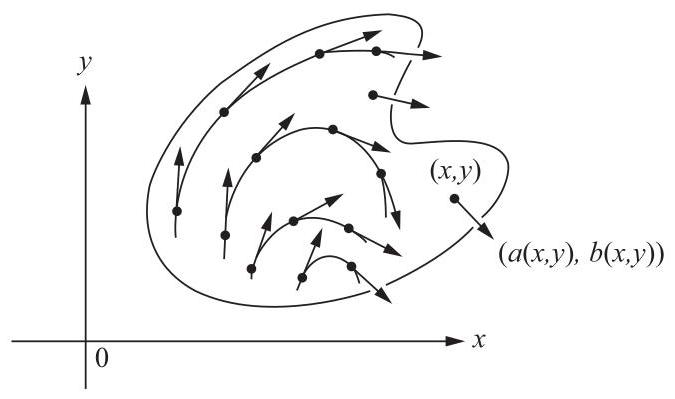
\includegraphics[max width=0.6\textwidth]{images/bo_d4b9jf3ef24c73e0334g_189_177_1496_675_399_0.jpg}
\end{center}
\hspace*{3em} 

图 3-24

在下文中，我们将只考虑可微向量场.图 3-25 展示了一些向量场的例子.



本节可在一读时略过.



\begin{center}
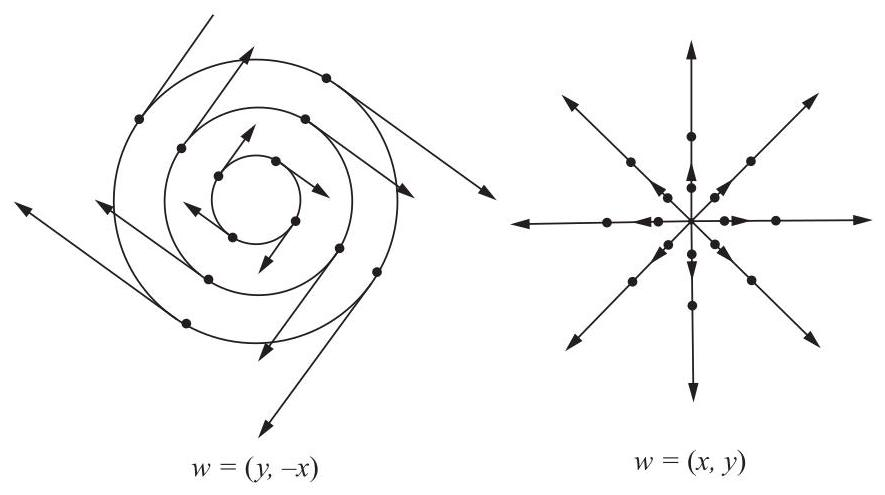
\includegraphics[max width=0.8\textwidth]{images/bo_d4b9jf3ef24c73e0334g_190_341_191_885_495_0.jpg}
\end{center}
\hspace*{3em} 

图 3-25

给定一个向量场 \(w\) ，自然会问是否存在该场的轨迹，即是否存在一个可微参数化曲线 \(\alpha \left( t\right)  = \left( {x\left( t\right) ,y\left( t\right) }\right) ,t \in  I\) ，使得 \({\alpha }^{\prime }\left( t\right)  = w\left( {\alpha \left( t\right) }\right)\) .

例如，通过点 \(\left( {{x}_{0},{y}_{0}}\right)\) 的向量场 \(w\left( {x,y}\right)  = \left( {x,y}\right)\) 的一条轨迹是直线 \(\alpha \left( t\right)  = \left( {{x}_{0}{e}^{t},{y}_{0}{e}^{t}}\right) ,t \in  R\) ，而通过 \(\left( {{x}_{0},{y}_{0}}\right)\) 的 \(w\left( {x,y}\right)  = \left( {y, - x}\right)\) 的一条轨迹是圆 \(\beta \left( t\right)  = \; \left( {r\sin t,r\cos t}\right) ,t \in  R,{r}^{2} = {x}_{0}^{2} + {y}_{0}^{2}\) .

用常微分方程的语言来说，向量场 \(w\) 确定了一个微分方程组，

\[
\frac{dx}{dt} = a\left( {x,y}\right) \tag{1}
\]

\[
\frac{dy}{dt} = b\left( {x,y}\right)
\]

而 \(w\) 的一条轨迹是方程 (1) 的一个解.

方程 (1) 解的(局部)存在唯一性定理等价于以下关于轨迹的陈述(在下文中，字母 \(I\) 和 \(J\) 将表示包含原点 \(0 \in  R\) 的直线 \(R\) 的开区间).

定理 1. 设 \(\mathrm{W}\) 是开集 \(\mathrm{U} \subset  {\mathbb{R}}^{2}\) 中的一个向量场.给定 \(\mathrm{p} \in  \mathrm{U}\) ，存在一个 \(\mathrm{w}\) 的轨迹 \(\alpha  : \mathrm{I} \rightarrow  \mathrm{U}\) (即 \({\alpha }^{\prime }\left( \mathrm{t}\right)  = \mathrm{w}\left( {\alpha \left( \mathrm{t}\right) }\right) ,\mathrm{t} \in  \mathrm{I}\) )，使得 \(\alpha \left( 0\right)  = \mathrm{p}\) .该轨迹在以下意义下是唯一的:任何另一条具有 \(\beta \left( 0\right)  = \mathrm{p}\) 的轨迹 \(\beta  : \mathrm{J} \rightarrow  \mathrm{U}\) 在 \(\mathrm{I} \cap  \mathrm{J}\) 上与 \(\alpha\) 一致.

定理 1 的一个重要补充是，通过 \(p\) 的轨迹“随 \(p\) 可微地变化”.这个想法可以精确地表述如下.

定理 2. 设 \(\mathrm{w}\) 是开集 \(\mathrm{U} \subset  {\mathbb{R}}^{2}\) 中的一个向量场.对于每个 \(\mathrm{p} \in  \mathrm{U}\) ，存在 \(\mathrm{p}\) 的一个邻域 \(\mathrm{V} \subset  \mathrm{U}\) 、一个区间 \(\mathrm{I}\) 和一个映射 \(\alpha  : \mathrm{V} \times  \mathrm{I} \rightarrow  \mathrm{U}\) ，使得

1. 对于固定的 \(\mathrm{q} \in  \mathrm{V}\) ，曲线 \(\alpha \left( {\mathrm{q},\mathrm{t}}\right) ,\mathrm{t} \in  \mathrm{I}\) 是 \(\mathrm{w}\) 通过 \(\mathrm{q}\) 的轨迹；即，

\[
\alpha \left( {\mathrm{q},0}\right)  = \mathrm{q},\;\frac{\partial \alpha }{\partial \mathrm{t}}\left( {\mathrm{q},\mathrm{t}}\right)  = \mathrm{w}\left( {\alpha \left( {\mathrm{q},\mathrm{t}}\right) }\right) .
\]

2. \(\alpha\) 是可微的.

定理 2 在几何上意味着，所有经过 \(t = 0\) 、在 \(p\) 的某个邻域 \(V\) 内的轨迹都可以被“收集”到一个可微映射中.正是在这个意义上，我们说轨迹可微地依赖于 \(p\) (图 3-26).

\begin{center}
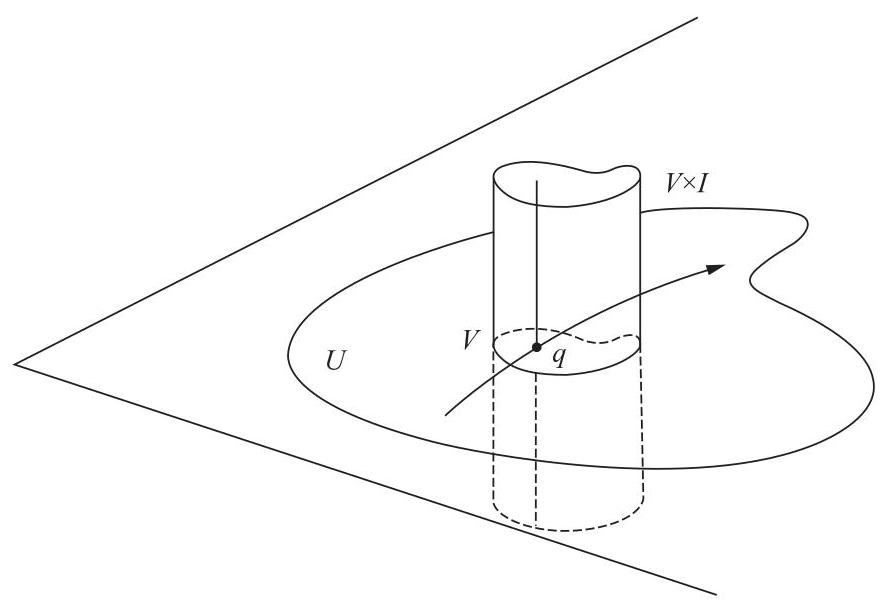
\includegraphics[max width=0.8\textwidth]{images/bo_d4b9jf3ef24c73e0334g_191_324_833_885_608_0.jpg}
\end{center}
\hspace*{3em} 

图 3-26

映射 \(\alpha\) 被称为 \(w\) 在 \(p\) 处的 (局部) 流.

本书将假定定理 1 和 2 成立；证明可参考，例如，W. Hurewicz, Lectures on Ordinary Differential Equations, M.I.T. Press, Cambridge, Mass., 1958, 第 2 章.对我们而言，我们需要这些定理的一个推论.

引理.设 \(\mathrm{w}\) 是开集 \(\mathrm{U} \subset  {\mathbb{R}}^{2}\) 中的一个向量场，且设 \(\mathrm{p} \in  \mathrm{U}\) 使得 \(\mathrm{w}\left( \mathrm{p}\right)  \neq  0\) .则存在 \(\mathrm{p}\) 的一个邻域 \(\mathrm{W} \subset  \mathrm{U}\) 和一个可微函数 \(\mathrm{f} : \mathrm{W} \rightarrow  \mathbb{R}\) ，使得 \(\mathrm{f}\) 沿 \(\mathrm{w}\) 的每条轨迹恒定，并且对于所有 \(\mathrm{q} \in  \mathrm{W}\) 成立 \({\mathrm{{df}}}_{\mathrm{q}} \neq  0\) .

证明.在 \({R}^{2}\) 中选择一个笛卡尔坐标系，使得 \(p = \left( {0,0}\right)\) 和 \(w\left( p\right)\) 沿 \(x\) 轴方向.设 \(\alpha  : V \times  I \rightarrow  U\) 是 \(p,V \subset  U,t \in  I\) 处的局部流，设 \(\widetilde{\alpha }\) 是 \(\alpha\) 在矩形上的限制

\[
\left( {V \times  I}\right)  \cap  \left\{  {\left( {x,y,t}\right)  \in  {R}^{3};x = 0}\right\}  .
\]

(见图 3-27.) 根据局部流的定义， \(d{\widetilde{\alpha }}_{p}\) 将 \(t\) 轴的单位向量映射到 \(w\) ，并将 \(y\) 轴的单位向量映射到自身.因此， \(d{\widetilde{\alpha }}_{p}\) 是非奇异的.由此可知，存在 \(p\) 的一个邻域 \(W \subset  U\) ，其中 \({\widetilde{\alpha }}^{-1}\) 是可定义的且可微的. \({\widetilde{\alpha }}^{-1}\left( {x,y}\right)\) 在 \(y\) 轴上的投影是一个可微函数 \(\xi  = f\left( {x,y}\right)\) ，它对于通过 \(\left( {0,\xi }\right)\) 的轨迹的所有点都具有相同的取值 \(\xi\) .由于 \(d{\widetilde{\alpha }}_{p}\) 是非奇异的，可以取 \(W\) 足够小，使得对于所有 \(q \in  W\) 成立 \(d{f}_{q} \neq  0\) .因此， \(f\) 是所求的函数.证毕.

\begin{center}
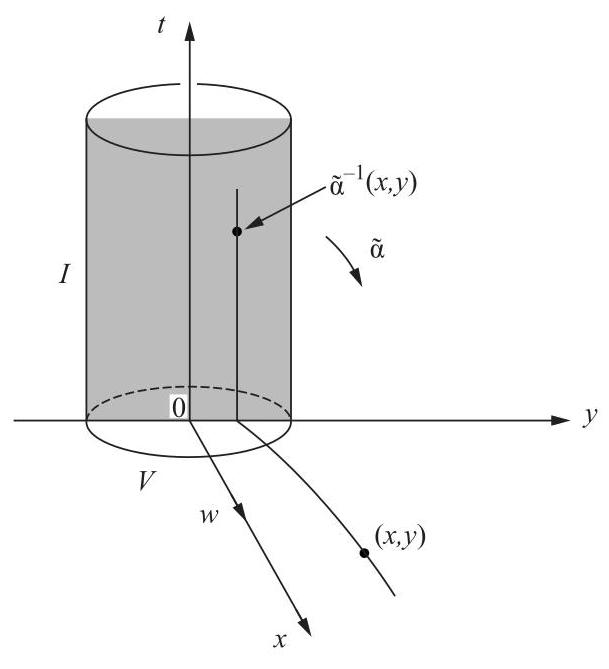
\includegraphics[max width=0.5\textwidth]{images/bo_d4b9jf3ef24c73e0334g_192_197_697_609_669_0.jpg}
\end{center}
\hspace*{3em} 

图 3-27

上述引理中的函数 \(f\) 被称为 \(w\) 在 \(p\) 邻域内的 (局部) 第一积分.例如，如果 \(w\left( {x,y}\right)  = \left( {y, - x}\right)\) 在 \({R}^{2}\) 中定义，则第一积分 \(f : {R}^{2} - \{ \left( {0,0}\right) \}  \rightarrow  R\) 是 \(f\left( {x,y}\right)  = {x}^{2} + {y}^{2}\) .

与向量场的概念紧密相关的是方向场的概念.

在开集 \(U \subset  {R}^{2}\) 中，方向场 \(r\) 是一个对应关系，它为每个 \(p \in  U\) 分配一条通过 \(p.r\) 的 \({R}^{2}\) 中的直线 \(r\left( p\right)\) .如果存在一个非零可微向量场 \(w\) ，在 \(p\) 的某个邻域 \(V \subset  U\) 中定义，使得对于每个 \(q \in  V,w\left( q\right)  \neq  0\) ， \(r\left( q\right) ;r\) 的基是可微的，则称该方向场在 \(p \in  U\) 处是可微的.如果它在每个 \(p \in  U\) 处都可微，则称它在 \(U\) 中是可微的.

对于 \(U \subset  {R}^{2}\) 中的每个非零可微向量场 \(w\) ，存在一个可微方向场，由 \(w\left( p\right)\) 生成的直线 \(r\left( p\right)  =\) ， \(p \in  U\) 给出.

根据其定义，每个可微方向场在局部上都会产生一个非零可微向量场.然而，这在全球范围内并不成立，如图 3-28 中由曲线的切线给出的 \({R}^{2} - \{ \left( {0,0}\right) \}\) 中的方向场所示；任何试图定向这些曲线以获得可微非零向量场的尝试都会导致矛盾.

正则连通曲线 \(C \subset  U\) 是定义在 \(U \subset  {R}^{2}\) 中的方向场 \(r\) 的积分曲线，如果对于所有 \(q \in  C\) ， \(r\left( q\right)\) 是 \(C\) 在 \(q\) 处的切线.

由前面所看到的内容可知，显然，在开集 \(U \subset  {R}^{2}\) 中给定一个可微方向场 \(r\) ，对于每个 \(q \in  U\) ，都存在一条 \(r;C\) 的积分曲线 \(C\) ，它在局部上与由 \(r\) 在 \(U\) 中确定的向量场通过 \(q\) 的轨迹的迹一致.接下来，我们将只考虑可微方向场，并且一般会省略“可微”这个词.

\begin{center}
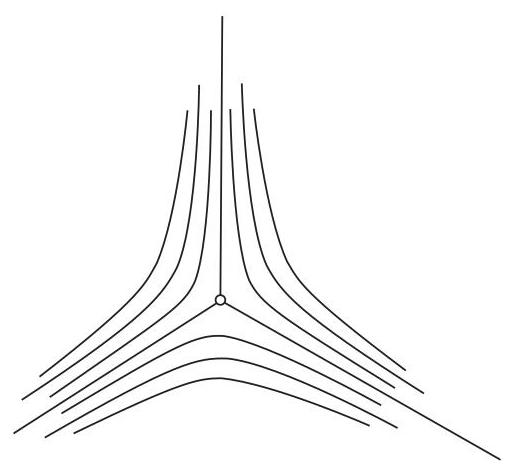
\includegraphics[max width=0.4\textwidth]{images/bo_d4b9jf3ef24c73e0334g_193_179_716_513_473_0.jpg}
\end{center}
\hspace*{3em} 

图 3-28. \({R}^{2} - \{ \left( {0,0}\right) \}\) 中的一个不可定向方向场.

描述方向场的一种自然方法如下.我们说在 \(q \in  {R}^{2}\) 处的两个非零向量 \({w}_{1}\) 和 \({w}_{2}\) 是等价的，如果存在某个 \(\lambda  \in  R,\lambda  \neq  0\) 使得 \({w}_{1} = \lambda {w}_{2}\) .这两个向量代表通过 \(q\) 的同一条直线，反之亦然，如果两个非零向量属于通过 \(q\) 的同一条直线，则它们是等价的.因此，开集 \(U \subset  {R}^{2}\) 上的方向场 \(r\) 可以通过为每个 \(q \in  U\) 分配一对实数 \(\left( {{r}_{1},{r}_{2}}\right)\) (属于 \(r\) 的非零向量的坐标)来给出，其中我们将对 \(\left( {{r}_{1},{r}_{2}}\right)\) 和 \(\left( {\lambda {r}_{1},\lambda {r}_{2}}\right) ,\lambda  \neq  0\) 视为等价的.

在微分方程的语言中，方向场 \(r\) 通常由以下方式给出:

\[
a\left( {x,y}\right) \frac{dx}{dt} + b\left( {x,y}\right) \frac{dy}{dt} = 0, \tag{2}
\]

这仅仅意味着在点 \(q = \left( {x,y}\right)\) 处，我们关联通过 \(q\) 的直线，该直线包含向量 \(\left( {b, - a}\right)\) 或其任何非零倍数(图 3-29).向量场 \(\left( {b, - a}\right)\) 的轨迹的迹线是 \(r\) 的积分曲线.由于参数化在上述考虑中不起作用，因此通常使用以下表达式代替方程 (2):

\[
{adx} + {bdy} = 0
\]

与之前的含义相同.

\begin{center}
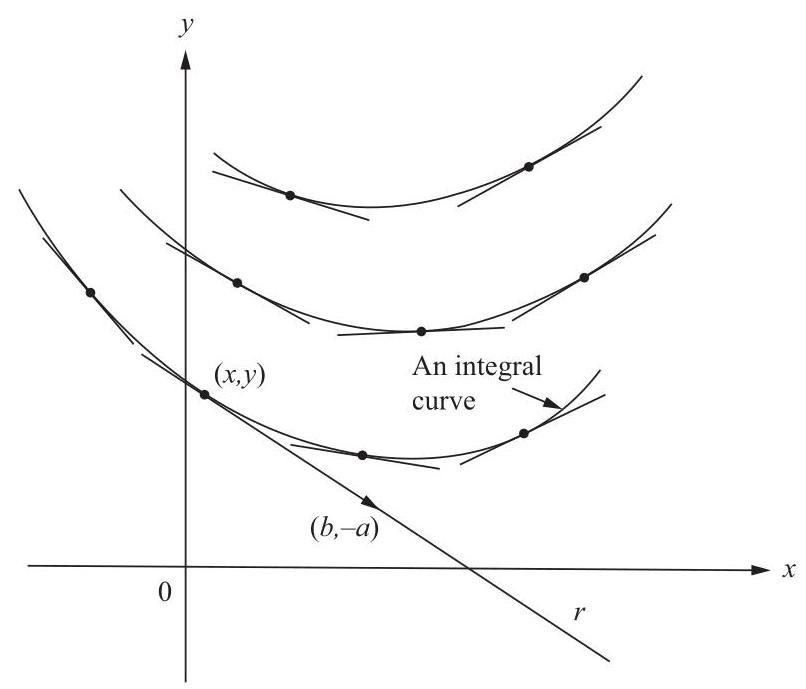
\includegraphics[max width=0.7\textwidth]{images/bo_d4b9jf3ef24c73e0334g_194_378_196_806_689_0.jpg}
\end{center}
\hspace*{3em} 

图 3-29. 微分方程 \({adx} + {bdy} = 0\) .

上述思想属于 \({R}^{2}\) 的局部事实范畴，仅取决于 \({R}^{2}\) 的“可微结构”.因此，它们可以毫无困难地推广到正则曲面上，如下所示.

定义 1. 正则曲面 \(S\) 的开集 \(\mathrm{U} \subset  S\) 中的向量场 \(\mathrm{w}\) 是一种对应关系，它为每个 \(\mathrm{p} \in  \mathrm{U}\) 分配一个向量 \(\mathrm{w}\left( \mathrm{p}\right)  \in \; {\mathrm{T}}_{\mathrm{p}}\left( S\right)\) .当对于 \(\mathrm{p}\) 的某个参数化 \(\mathbf{x}\left( {\mathrm{u},\mathrm{v}}\right)\) ，由以下给出的函数 \(\mathrm{a}\left( {\mathrm{u},\mathrm{v}}\right)\) 和 \(\mathrm{b}\left( {\mathrm{u},\mathrm{v}}\right)\) 在 \(\mathrm{p} \in  \mathrm{U}\) 处可微时，向量场 \(\mathrm{w}\) 在 \(\mathrm{p} \in  \mathrm{U}\) 处是可微的；显然，这个定义不依赖于 \(\mathrm{U} \subset  S\) 的选择.

\[
w\left( p\right)  = a\left( {u,v}\right) {\mathbf{x}}_{u} + b\left( {u,v}\right) {\mathbf{x}}_{v}
\]

在 \(\mathrm{p}\) 处是可微函数；很明显，这个定义不依赖于 \(\mathbf{x}\) 的选择.

类似地，我们可以定义轨迹、方向场和积分曲线.定理 1 和定理 2 以及上面的引理可以很容易地推广到当前情况；除了 \({R}^{2}\) 被 \(S\) 替换外，陈述完全相同.

例 1. 在普通环面 \(T\) 中，通过按弧长参数化子午线 \(T\) 并将 \(w\left( p\right)\) 定义为通过 \(p\) 的子午线的速度向量(图 3-30)来获得向量场.请注意，对于所有 \(p \in  T\) ，都有 \(\left| {w\left( p\right) }\right|  = 1\) .将其留作练习(练习 2)来验证 \(w\) 是可微的.

例 2. 类似的过程，这次在球面 \({S}^{2}\) 上并使用 \({S}^{2}\) 的半子午线，会产生一个定义在除去两个极点 \(N\) 和 \(S\) 的球面上的向量场 \(w\) .为了获得定义在整个球面上的向量场，用相同的参数 \(t, - 1 < t < 1\) 重新参数化所有半子午线，并为 \(p \in  {S}^{2} - \{ N\}  \cup  \{ S\}\) 和 \(v\left( N\right)  = v\left( S\right)  = 0\) 定义 \(v\left( p\right)  = \left( {1 - {t}^{2}}\right) w\left( p\right)\) (图 3-31).

\begin{center}
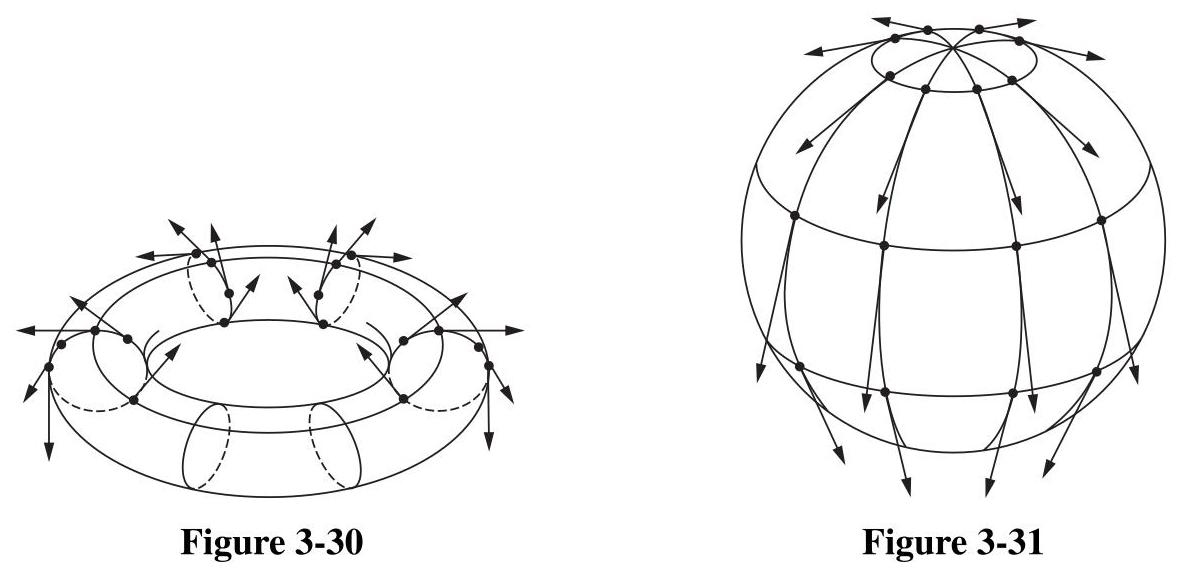
\includegraphics[max width=1.0\textwidth]{images/bo_d4b9jf3ef24c73e0334g_195_173_189_1181_574_0.jpg}
\end{center}
\hspace*{3em} 

示例 3. 令 \(S = \left\{  {\left( {x,y,z}\right)  \in  {R}^{3};z = {x}^{2} - {y}^{2}}\right\}\) 为双曲抛物面.与 \(S\) 相交的平面 \(z =\) = const. \(\neq  0\) 确定了一族曲线 \(\left\{  {C}_{\alpha }\right\}\) ，使得通过 \(S - \{ \left( {0,0,0}\right) \}\) 的每一点都有一条曲线 \({C}_{\alpha }\) .这些曲线的切线在 \(S - \{ \left( {0,0,0}\right) \}\) 上给出了一个可微的方向场 \(r\) .我们想在 \(S - \{ \left( {0,0,0}\right) \}\) 上找到一个方向场 \({r}^{\prime }\) ，它在每一点都与 \(r\) 正交，并确定 \({r}^{\prime }.{r}^{\prime }\) 的积分曲线被称为 \(r\) 的正交场，其积分曲线被称为 \(r\) 的正交族(参见练习 15，第 2-5 节).

我们首先通过参数化 \(S\) 来开始

\[
\mathbf{x}\left( {u,v}\right)  = \left( {u,v,{u}^{2} - {v}^{2}}\right) ,\;u = x,\;v = y.
\]

族 \(\left\{  {C}_{\alpha }\right\}\) 由 \({u}^{2} - {v}^{2} =\) = const. \(\neq  0\) 给出(或者更确切地说，由该集合在 \(\mathbf{x}\) 下的像给出).如果 \({u}^{\prime }{\mathbf{x}}_{u} + {v}^{\prime }{\mathbf{x}}_{v}\) 是某条曲线 \({C}_{\alpha }\) 的正则参数化的切向量，通过对 \({u}^{2} - {v}^{2} =\) = const. 求导，我们得到:

\[
{2u}{u}^{\prime } - {2v}{v}^{\prime } = 0.
\]

因此， \(\left( {{u}^{\prime },{v}^{\prime }}\right)  = \left( {-v, - u}\right)\) .由此可知，在参数化 \(\mathbf{x}\) 中， \(r\) 由对 \(\left( {v,u}\right)\) 或其任何非零倍数给出.

现在，令 \(\left( {a\left( {u,v}\right) ,b\left( {u,v}\right) }\right)\) 为正交场 \({r}^{\prime }\) 在参数化 \(\mathbf{x}\) 中的表达式.由于

\[
E = 1 + 4{u}^{2},\;F =  - {4uv},\;G = 1 + 4{v}^{2},
\]

并且 \({r}^{\prime }\) 在每一点都与 \(r\) 正交，我们有

\[
{Eav} + F\left( {{bv} + {au}}\right)  + {Gbu} = 0
\]

or

\[
\left( {1 + 4{u}^{2}}\right) {av} - {4uv}\left( {{bv} + {au}}\right)  + \left( {1 + 4{v}^{2}}\right) {bu} = 0.
\]

由此可知

\[
{va} + {ub} = 0. \tag{3}
\]

这确定了每一点的对 \(\left( {a,b}\right)\) ，在非零倍数意义下，因此也确定了场 \({r}^{\prime }\) .

为了找到 \({r}^{\prime }\) 的积分曲线，令 \({u}^{\prime }{\mathbf{x}}_{u} + {v}^{\prime }{\mathbf{x}}_{v}\) 为 \({r}^{\prime }\) 的积分曲线的某个正则参数化的切向量.那么 \(\left( {{u}^{\prime },{v}^{\prime }}\right)\) 满足方程 (3)；即:

\[
v{u}^{\prime } + u{v}^{\prime } = 0
\]

or

\[
{uv} = \text{ const. }
\]

由此可知， \(\left\{  {C}_{\alpha }\right\}\) 的正交族由与 \(S\) 相交的双曲圆柱面 \({xy} =\) = const. \(\neq  0\) 给出.

本节的主要结果是以下定理.

定理. 设 \({\mathrm{w}}_{1}\) 和 \({\mathrm{w}}_{2}\) 是开集 \(\mathrm{U} \subset  S\) 中的两个向量场，它们在某点 \(\mathrm{p} \in  \mathrm{U}\) 处线性无关. 那么可以对 \(\mathrm{p}\) 的一个邻域 \(\mathrm{V} \subset  \mathrm{U}\) 进行参数化，使得对于每个 \(\mathrm{q} \in  \mathrm{V}\) ，通过 \(\mathrm{q}\) 的该参数化的坐标曲线都与由 \({\mathrm{w}}_{1}\left( \mathrm{q}\right)\) 和 \({\mathrm{w}}_{2}\left( \mathrm{q}\right)\) 确定的直线相切.

证明. 设 \(W\) 是 \(p\) 的一个邻域，其中定义了 \({w}_{1}\) 和 \({w}_{2}\) 的各自的第一个积分 \({f}_{1}\) 和 \({f}_{2}\) . 定义一个映射 \(\varphi  : W \rightarrow  {R}^{2}\) 如下:

\[
\varphi \left( q\right)  = \left( {{f}_{1}\left( q\right) ,{f}_{2}\left( q\right) }\right) ,\;q \in  W.
\]

由于 \({f}_{1}\) 在 \({w}_{1}\) 和 \(\left( {d{f}_{1}}\right)  \neq  0\) 的轨迹上是常数，我们在 \(p\) 处有

\[
d{\varphi }_{p}\left( {w}_{1}\right)  = \left( {{\left( d{f}_{1}\right) }_{p}\left( {w}_{1}\right) ,{\left( d{f}_{2}\right) }_{p}\left( {w}_{1}\right) }\right)  = \left( {0,a}\right) ,
\]

其中 \(a = {\left( d{f}_{2}\right) }_{p}\left( {w}_{1}\right)  \neq  0\) ，因为 \({w}_{1}\) 和 \({w}_{2}\) 线性无关. 类似地，

\[
d{\varphi }_{p}\left( {w}_{2}\right)  = \left( {b,0}\right) ,
\]

其中 \(b = {\left( d{f}_{1}\right) }_{p}\left( {w}_{2}\right)  \neq  0\) .

由此可知 \(d{\varphi }_{p}\) 是非奇异的，因此 \(\varphi\) 是一个局部微分同胚. 所以存在 \(\varphi \left( p\right)\) 的一个邻域 \(\bar{U} \subset  {R}^{2}\) ，它被 \(\mathbf{x} = {\varphi }^{-1}\) 微分同胚地映射到一个 \(p\) 的邻域 \(V = \mathbf{x}\left( \bar{U}\right)\) ；也就是说， \(\mathbf{x}\) 是 \(S\) 在 \(p\) 处的一个参数化，其坐标曲线

\[
{f}_{1}\left( q\right)  = \text{ const., }\;{f}_{2}\left( q\right)  = \text{ const., }
\]

分别在 \(q\) 处与由 \({w}_{1}\left( q\right) ,{w}_{2}\left( q\right)\) 确定的直线相切. 证毕.

应该指出的是，该定理并不意味着坐标曲线可以被参数化，使得它们的切向量是 \({w}_{1}\left( q\right)\) 和 \({w}_{2}\left( q\right)\) . 该定理的陈述适用于坐标曲线作为正则(点集)曲线；更精确地说，我们有

推论 1. 设在开集 \(\mathrm{U} \subset  S\) 中给定两个方向场 \(\mathrm{r}\) 和 \({\mathrm{r}}^{\prime }\) ，使得在 \(\mathrm{p} \in  \mathrm{U},\mathrm{r}\left( \mathrm{p}\right)  \neq  {\mathrm{r}}^{\prime }\left( \mathrm{p}\right)\) 处，存在一个邻域 \(\mathrm{p}\) 的参数化 \(\mathbf{x}\) ，使得 \(\mathbf{x}\) 的坐标曲线是 \(\mathrm{r}\) 和 \({\mathrm{r}}^{\prime }\) 的积分曲线.

上述定理的一个初步应用是证明在正则曲面的任意一点处存在一个正交参数化.

推论 2. 对于所有 \(\mathrm{p} \in  S\) ，在 \(\mathrm{p}\) 的邻域 \(\mathrm{V}\) 中存在一个参数化 \(\mathbf{x}\left( {\mathrm{u},\mathrm{v}}\right)\) ，使得坐标曲线 \(\mathrm{u} =\) 为常数， \(\mathrm{v} =\) 为常数，对于每个 \(\mathrm{q} \in  \mathrm{V}\) ，它们正交相交(这样的 \(\mathbf{x}\) 称为正交参数化).

证明. 考虑 \(p\) 处任意一个参数化 \(\overline{\mathbf{x}} : \bar{U} \rightarrow  S\) ，并在 \(\overline{\mathbf{x}}\left( \bar{U}\right)\) 中定义两个向量场 \({w}_{1} = {\overline{\mathbf{x}}}_{\bar{u}},{w}_{2} =  - \left( {\bar{F}/\bar{E}}\right) {\overline{\mathbf{x}}}_{\bar{u}} + {\overline{\mathbf{x}}}_{\bar{v}}\) ，其中 \(\bar{E},\bar{F},\bar{G}\) 是 \(\overline{\mathbf{x}}\) 中第一基本形式的系数.由于 \({w}_{1}\left( q\right) ,{w}_{2}\left( q\right)\) 是正交向量，对于每个 \(q \in  \overline{\mathbf{x}}\left( \bar{U}\right)\) ，应用该定理即可得到所需的参数化.证毕.

该定理(更准确地说，是推论 1)的第二次应用是渐近线方向和主方向给出的坐标的存在性.

正如我们在第 3-3 节中所见，渐近线是以下方程的解:

\[
e{\left( {u}^{\prime }\right) }^{2} + {2f}{u}^{\prime }{v}^{\prime } + g{\left( {v}^{\prime }\right) }^{2} = 0.
\]

在双曲点 \(p\) 的邻域中，我们有 \({eg} - {f}^{2} < 0\) .旋转平面 \({uv}\) ，使得 \(e\left( p\right)  > 0\) .那么上述方程的左侧可以分解为两个不同的线性因子，得到:

\[
\left( {A{u}^{\prime } + B{v}^{\prime }}\right) \left( {A{u}^{\prime } + D{v}^{\prime }}\right)  = 0, \tag{4}
\]

其中系数由以下公式确定:

\[
{A}^{2} = e,\;A\left( {B + D}\right)  = {2f},\;{BD} = g.
\]

上述方程组有实数解，因为 \({eg} - {f}^{2} < 0\) .因此，方程 (4) 产生两个方程:

\[
A{u}^{\prime } + B{v}^{\prime } = 0, \tag{4a}
\]

\[
A{u}^{\prime } + D{v}^{\prime } = 0. \tag{4b}
\]

每个方程确定一个可微方向场(例如，方程 (4a) 确定包含非零向量 \(\left( {B, - A}\right)\) 的方向 \(r\) )，并且在所讨论的邻域的每一点，由方程 (4a) 和 (4b) 给出的方向是不同的.通过应用推论 1，我们看到可以对 \(p\) 的邻域进行参数化，使得坐标曲线是方程 (4a) 和 (4b) 的积分曲线.换句话说，

推论 3. 令 \(\mathrm{p} \in  S\) 为 \(S\) 的一个双曲点.那么可以对 \(\mathrm{p}\) 的邻域进行参数化，使得该参数化的坐标曲线是 S 的渐近线.

例 4. 一个几乎微不足道的例子，但它说明了上述方法的机制，是由双曲抛物面 \(z = {x}^{2} - {y}^{2}\) 给出的.像往常一样，我们用以下方式对整个曲面进行参数化:

\[
\mathbf{x}\left( {u,v}\right)  = \left( {u,v,{u}^{2} - {v}^{2}}\right) .
\]

简单的计算表明:

\[
e = \frac{2}{{\left( 1 + 4{u}^{2} + 4{v}^{2}\right) }^{1/2}},\;f = 0,\;g =  - \frac{2}{{\left( 1 + 4{u}^{2} + 4{v}^{2}\right) }^{1/2}}.
\]

因此，渐近线的方程可以写成:

\[
\frac{2}{{\left( 1 + 4{u}^{2} + 4{v}^{2}\right) }^{1/2}}\left( {{\left( {u}^{\prime }\right) }^{2} - {\left( {v}^{\prime }\right) }^{2}}\right)  = 0,
\]

它可以分解为两个线性方程，并给出两个方向场:

\[
{r}_{1} : {u}^{\prime } + {v}^{\prime } = 0
\]

\[
{r}_{2} : {u}^{\prime } - {v}^{\prime } = 0
\]

这些方向场的积分曲线由以下两族曲线给出:

\[
{r}_{1} : u + v = \text{ const., }
\]

\[
{r}_{2} : u - v = \text{ const. }
\]

现在，函数 \({f}_{1}\left( {u,v}\right)  = u + v,{f}_{2}\left( {u,v}\right)  = u - v\) 显然是与向量场 \({r}_{1}\) 和 \({r}_{2}\) 相关的向量场的第一积分，分别.因此，通过设置

\[
\bar{u} = u + v,\;\bar{v} = u - v,
\]

我们得到整个曲面 \(z = {x}^{2} - {y}^{2}\) 的新参数化，其中坐标曲线是曲面的渐近线.

在此特定情况下，参数的变化适用于整个曲面.一般而言，即使整个曲面仅由双曲点组成，它也可能无法全局一对一.

类似地，在 \(S\) 的非脐点附近，可以将曲率线的微分方程分解为不同的线性因子.通过类似的论证，我们得到

推论 4. 令 \(\mathrm{p} \in  S\) 为 \(S\) 的一个非脐点.则可以对 \(\mathrm{p}\) 的邻域进行参数化，使得该参数化的坐标曲线是 \(S\) 的曲率线.

\exerciseline

1. 证明向量场的微分性不依赖于坐标系的选择.

2. 证明通过将环面上的所有经线按弧长参数化并取其切向量(例 1)得到的向量场是可微的.

3. 证明在正则曲面 \(S \subset  {R}^{3}\) 上定义的向量场 \(w\) 是可微的，当且仅当它作为映射 \(w : S \rightarrow  {R}^{3}\) 是可微的.

4. 令 \(S\) 为一个曲面， \(\mathbf{x} : U \rightarrow  S\) 为 \(S\) 的一个参数化.则

\[
a\left( {u,v}\right) {u}^{\prime } + b\left( {u,v}\right) {v}^{\prime } = 0,
\]

其中 \(a\) 和 \(b\) 是可微函数，在 \(\mathbf{x}\left( U\right)\) 上确定了一个方向场 \(r\) ，即，将每个 \(\mathbf{x}\left( {u,v}\right)\) 映射到包含向量 \(b{\mathbf{x}}_{u} - a{\mathbf{x}}_{v}\) 的直线.证明存在 \(\mathbf{x}\left( U\right)\) 上的正交场 \({r}^{\prime }\) (参见例 3)的充要条件是两个函数

\[
{Eb} - {Fa},\;{Fb} - {Ga}
\]

永不同时为零(此处 \(E,F\) 和 \(G\) 是 \(\mathbf{x}\) 中第一基本形式的系数)，并且 \({r}^{\prime }\) 由下式确定

\[
\left( {{Eb} - {Fa}}\right) {u}^{\prime } + \left( {{Fb} - {Ga}}\right) {v}^{\prime } = 0.
\]

5. 令 \(S\) 为一个曲面， \(\mathbf{x} : U \rightarrow  S\) 为 \(S\) 的一个参数化.如果 \({ac} - {b}^{2} < 0\) ，则证明

\[
a\left( {u,v}\right) {\left( {u}^{\prime }\right) }^{2} + {2b}\left( {u,v}\right) {u}^{\prime }{v}^{\prime } + c\left( {u,v}\right) {\left( {v}^{\prime }\right) }^{2} = 0
\]

可以分解为两个不同的方程，每个方程确定 \(\mathbf{x}\left( U\right)  \subset  S\) 上的一个方向场.证明这两个方向场正交当且仅当

\[
{Ec} - {2Fb} + {Ga} = 0.
\]

3-4. 向量场

\begin{center}
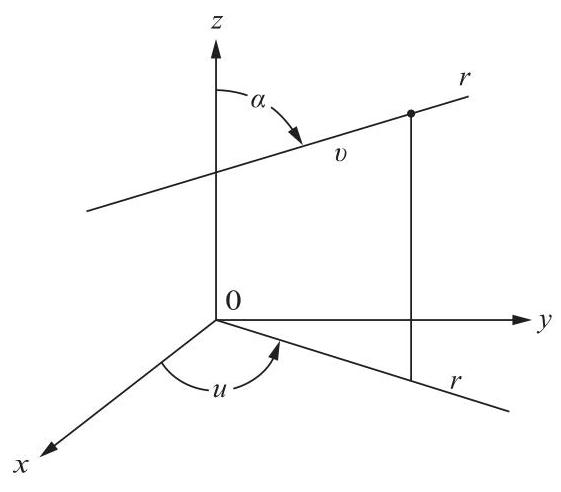
\includegraphics[max width=0.5\textwidth]{images/bo_d4b9jf3ef24c73e0334g_200_196_202_561_492_0.jpg}
\end{center}
\hspace*{3em} 

图 3-32

6. 一条直线 \(r\) 与 \(z\) 轴相交，并以这样的方式移动，使其与 \(z\) 轴成恒定角度 \(\alpha  \neq  0\) ，并且其每个点都围绕 \(z\) 轴描述一个螺距为 \(c \neq  0\) 的螺旋线. \(r\) 所描述的图形是参数化曲面(见图 3-32)的轨迹.

\[
\mathbf{x}\left( {u,v}\right)  = \left( {v\sin \alpha \cos u,v\sin \alpha \sin u,v\cos \alpha  + {cu}}\right) .
\]

\(\mathbf{x}\) 很容易被看作是一个正则参数化曲面(参见第 2-5 节练习题 13).将参数 \(\left( {u,v}\right)\) 限制在一个开集 \(U\) 上，使得 \(\mathbf{x}\left( U\right)  = \; S\) 是一个正则曲面(参见第 2-3 节命题 2).

a. 找到坐标曲线族 \(u =\) = const. 的正交族(参见例 3).

b. 使用曲线 \(u =\) = const. 及其正交族来获得 \(S\) 的正交参数化.证明在新参数 \(\left( {\bar{u},\bar{v}}\right)\) 下，第一基本形式的系数为

\[
\bar{G} = 1,\;\bar{F} = 0,\;\bar{E} = \left\{  {{c}^{2} + {\left( \bar{v} - c\bar{u}\cos \alpha \right) }^{2}}\right\}  {\sin }^{2}\alpha .
\]

7. 在 \(\mathrm{U}\) 中，相对于向量场 \(\mathrm{w}\) 定义可微函数 \(\mathrm{f} : \mathrm{U} \subset  S \rightarrow  \mathbb{R}\) 的导数 \(\mathrm{w}\left( \mathrm{f}\right)\) 为

\[
\mathrm{w}\left( \mathrm{f}\right) \left( \mathrm{q}\right)  = {\left. \frac{\mathrm{d}}{dt}\left( \mathrm{f} \circ  \alpha \right) \right| }_{\mathrm{t} = 0},\;\mathrm{q} \in  \mathrm{U},
\]

其中 \(\alpha  : I \rightarrow  S\) 是一条曲线，使得 \(\alpha \left( 0\right)  = q,{\alpha }^{\prime }\left( 0\right)  = w\left( q\right)\) .证明

a. \(w\) 在 \(U\) 中可微当且仅当对于 \(U\) 中所有可微的 \(f\) ， \(w\left( f\right)\) 是可微的.

b. 令 \(\lambda\) 和 \(\mu\) 为实数，令 \(g : U \subset  S \rightarrow  R\) 为 \(U\) 上的可微函数；则

\[
w\left( {{\lambda f} + {\mu f}}\right)  = {\lambda w}\left( f\right)  + {\mu w}\left( f\right) ,
\]

\[
w\left( {fg}\right)  = w\left( f\right) g + {fw}\left( g\right) .
\]

8. 证明如果 \(w\) 是曲面 \(S\) 上的一个可微向量场，并且对于某个 \(p \in  S\) 有 \(w\left( p\right)  \neq  0\) ，那么可以对 \(p\) 的一个邻域进行参数化，使用 \(\mathbf{x}\left( {u,v}\right)\) ，使得 \({\mathbf{x}}_{u} = w\) .

9. a. 令 \(A : V \rightarrow  W\) 为向量空间 \(V\) 和 \(W\) 的非奇异线性映射，它们的维度均为 2，并分别赋予内积 \(\langle\) 和 \(\rangle {and}\left( ,\right) ,\) .如果存在实数 \(\lambda  \neq  0\) 使得对于所有向量 \({v}_{1},{v}_{2} \in  V\) 都有 \(\left( {A{v}_{1},A{v}_{2}}\right)  = \lambda \left\langle  {{v}_{1},{v}_{2}}\right\rangle\) ，则称 \(A\) 是相似映射.假设 \(A\) 不是相似映射，并证明存在一对唯一的标准正交向量 \({e}_{1}\) 和 \({e}_{2}\) 在 \(V\) 中，使得 \(A{e}_{1},A{e}_{2}\) 在 \(W\) 中正交.

b. 利用 a 部分证明 Tissot 定理:令 \(\varphi  : {U}_{1} \subset  {S}_{1} \rightarrow  {S}_{2}\) 为曲面 \({S}_{1}\) 上点 \(p\) 的邻域 \({U}_{1}\) 到曲面 \({S}_{2}\) 的一个微分同胚.假设线性映射 \({d\varphi }\) 在任何地方都不是相似映射.则可以对 \({S}_{1}\) 中点 \(p\) 的邻域进行参数化，得到一个正交参数化 \({\mathbf{x}}_{1} : U \rightarrow  {S}_{1}\) ，使得 \(\varphi  \circ  {\mathbf{x}}_{1} = {\mathbf{x}}_{2} : U \rightarrow  {S}_{2}\) 也是 \(\varphi \left( p\right)  \in  {S}_{2}\) 的邻域中的一个正交参数化.

10. 令 \(T\) 为 2-2 节示例 6 中的环面，并定义一个映射 \(\varphi  : {R}^{2} \rightarrow  T\) 为

\[
\varphi \left( {u,v}\right)  = \left( {\left( {r\cos u + a}\right) \cos v,\left( {r\cos u + a}\right) \sin v,r\sin u}\right) ,
\]

其中 \(u\) 和 \(v\) 是 \({R}^{2}\) 的笛卡尔坐标.令 \(u = {at},v = {bt}\) 为通过 \(\left( {0,0}\right)  \in  {R}^{2}\) 的 \({R}^{2}\) 中的一条直线，并考虑 \({T\alpha }\left( t\right)  = \varphi \left( {{at},{bt}}\right)\) 中的曲线.证明

a. \(\varphi\) 是局部微分同胚.

b. 曲线 \(\alpha \left( t\right)\) 是一条正则曲线；当且仅当 \(b/a\) 是有理数时， \(\alpha \left( t\right)\) 是闭合曲线.

*c. 如果 \(b/a\) 是无理数，则曲线 \(\alpha \left( t\right)\) 在 \(T\) 中是稠密的；也就是说，在点 \(p \in  T\) 的每个邻域中都存在 \(\alpha \left( t\right)\) 的一个点.

*11. 利用向量场 \(w\) 在 \(U \subset  S\) 处的轨线的局部唯一性，证明以下结果.给定 \(p \in  U\) ，存在 \(w\) 的唯一轨线 \(\alpha  : I \rightarrow  U\) ，满足 \(\alpha \left( 0\right)  = p\) ，并且在以下意义下是极大的:任何其他轨线 \(\beta  : J \rightarrow  U\) ，满足 \(\beta \left( 0\right)  = p\) ，是 \(\alpha\) 在 \(J\) 上的限制(即， \(J \subset  I\) 且 \(\alpha  \mid  J = \beta\) ).

*12. 证明如果 \(w\) 是紧致曲面 \(S\) 上的可微向量场，并且 \(\alpha \left( t\right)\) 是 \(w\) 具有 \(\alpha \left( 0\right)  = p \in  S\) 的极大轨线，则 \(\alpha \left( t\right)\) 对所有 \(t \in  R\) 都有定义.

13. 在平面上(非紧致)的开圆盘上构造一个可微向量场，使得一条极大轨线 \(\alpha \left( t\right)\) 对所有 \(t \in  R\) 都没有定义(这表明练习 12 的紧致性条件是必不可少的).

\section*{3-5. 直纹曲面与极小曲面†}

在微分几何中，有相当多的特例(旋转曲面、平行曲面、直纹曲面、极小曲面等)，它们本身可能很有趣(如极小曲面)，或者能很好地展示微分几何方法的力量和局限性.根据本书的精神，到目前为止，我们已在示例和练习中处理了这些特例.

然而，将其中一些主题更详细地介绍可能会很有用.我们打算现在就这样做.我们将使用本节来发展直纹曲面理论并介绍极小曲面理论.在本节中，使用第 2-3 节中定义的参数化曲面概念将很方便.

如果读者愿意，可以省略整个章节或其中一个主题.除了在 B 节的示例 6 中引用 A 节之外，这两个主题是独立的，并且它们的结果不会以任何重要的方式在本书中被使用.

\section*{A. 直纹曲面}

\(A\) (可微的)单参数直线族 \(\{ \alpha \left( t\right) ,w\left( t\right) \}\) 是一种对应关系，它为每个 \(t \in  I\) 分配一个点 \(\alpha \left( t\right)  \in  {R}^{3}\) 和一个向量 \(w\left( t\right)  \in  {R}^{3},w\left( t\right)  \neq  0\) ，使得 \(\alpha \left( t\right)\) 和 \(w\left( t\right)\) 都可微地依赖于 \(t\) .对于每个 \(t \in  I\) ，通过 \(\alpha \left( t\right)\) 且平行于 \(w\left( t\right)\) 的直线 \({L}_{t}\) 被称为 \(t\) 处的族线.

给定一个单参数直线族 \(\{ \alpha \left( t\right) ,w\left( t\right) \}\) ，参数化曲面

\[
\mathbf{x}\left( {t,v}\right)  = \alpha \left( t\right)  + {vw}\left( t\right) ,\;t \in  I,\;v \in  R,
\]

被称为由族 \(\{ \alpha \left( t\right) ,w\left( t\right) \}\) 生成的直纹曲面.直线 \({L}_{t}\) 被称为生成线，曲线 \(\alpha \left( t\right)\) 被称为曲面 \(\mathbf{x}\) 的准线.有时我们使用直纹曲面这个词来表示 \(\mathbf{x}\) 的轨迹.应该注意的是，我们也允许 \(\mathbf{x}\) 具有奇异点，即 \(\left( {t,v}\right)\) 处 \({\mathbf{x}}_{t} \land  {x}_{v} = 0\) 的点.



†本节在初读时可以省略.



示例 1. 直纹曲面的最简单示例是正则曲线的切面(参见示例 4，第 2-3 节)、柱面和锥面.柱面是由参数为一的一族直线 \(\{ \alpha \left( t\right) ,w\left( t\right) \} ,t \in  I\) 生成的直纹曲面，其中 \(\alpha \left( I\right)\) 包含在平面 \(P\) 中，并且 \(w\left( t\right)\) 平行于 \({R}^{3}\) 中的固定方向(图 3-33(a)).锥面是由一族 \(\{ \alpha \left( t\right) ,w\left( t\right) \} ,t \in  I\) 生成的直纹曲面，其中 \(\alpha \left( I\right)  \subset  P\) 和所有生成线 \({L}_{t}\) 都通过点 \(p \notin  P\) (图 3-33(b)).

\begin{center}
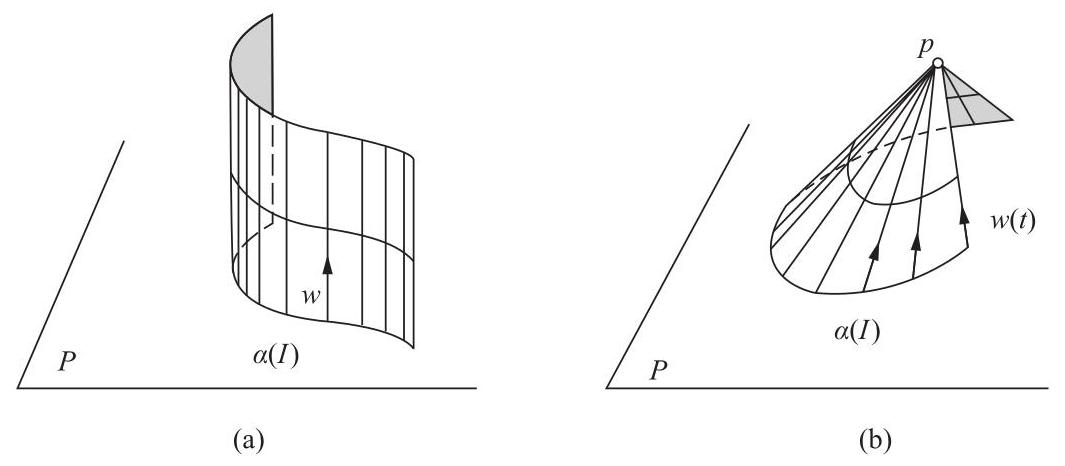
\includegraphics[max width=0.9\textwidth]{images/bo_d4b9jf3ef24c73e0334g_203_237_658_1065_466_0.jpg}
\end{center}
\hspace*{3em} 

图 3-33

示例 2. 令 \({S}^{1}\) 为 \({xy}\) 平面中的单位圆 \({x}^{2} + {y}^{2} = 1\) ，令 \(\alpha \left( s\right)\) 为 \({S}^{1}\) 的弧长参数化.对于每个 \(s\) ，令 \(w\left( s\right)  = {\alpha }^{\prime }\left( s\right)  + {e}_{3}\) ，其中 \({e}_{3}\) 是 \(z\) 轴的单位向量(图 3-34).那么

\[
\mathbf{x}\left( {s,v}\right)  = \alpha \left( s\right)  + v\left( {{\alpha }^{\prime }\left( s\right)  + {e}_{3}}\right)
\]

是一个直纹曲面.如果我们写成

\[
\mathbf{x}\left( {s,v}\right)  = \left( {\cos s - v\sin s,\sin s + v\cos s,v}\right)
\]

\begin{center}
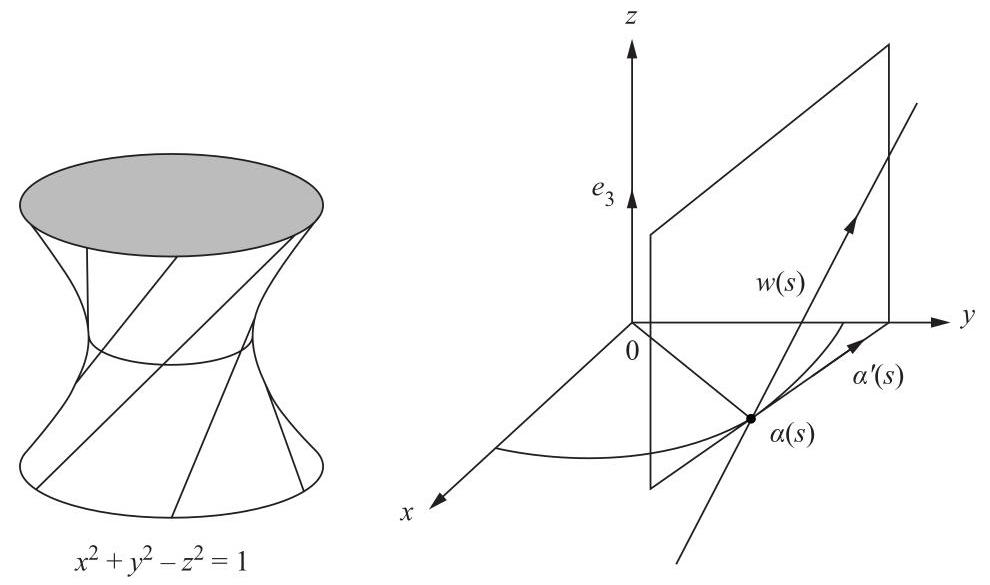
\includegraphics[max width=0.8\textwidth]{images/bo_d4b9jf3ef24c73e0334g_203_272_1454_990_585_0.jpg}
\end{center}
\hspace*{3em} 

图 3-34. \({x}^{2} + {y}^{2} - {z}^{2} = 1\) 作为直纹曲面.

并注意到 \({x}^{2} + {y}^{2} - {z}^{2} = 1 + {v}^{2} - {v}^{2} = 1\) .这表明 \(\mathbf{x}\) 的轨迹是旋转双曲面.

有趣的是，如果我们取 \(w\left( s\right)  =  - {\alpha }^{\prime }\left( s\right)  + {e}_{3}\) ，我们又得到了相同的曲面.这表明旋转双曲面有两组生成线.

我们定义直纹曲面的方式允许出现奇点.如果我们想包含切面和锥面，这是必要的.我们很快就会证明，至少对于满足某些合理条件的直纹曲面来说，这样的曲面的奇点(如果有的话)将集中在该曲面的一条曲线上.

我们现在开始研究一般的直纹曲面.我们可以不失一般性地假设 \(\left| {w\left( t\right) }\right|  = 1,t \in  I\) .为了能够发展理论，我们需要非平凡的假设，即对于所有 \(t \in  I\) ， \({w}^{\prime }\left( t\right)  \neq  0\) .如果 \({w}^{\prime }\left( t\right)\) 的零点是孤立的，我们可以将曲面分成几块，以便理论可以应用于每一块.然而，如果 \({w}^{\prime }\left( t\right)\) 的零点有聚点，情况可能会变得复杂，这里将不作处理.

假设 \({w}^{\prime }\left( t\right)  \neq  0,t \in  I\) ，通常通过说直纹曲面 \(\mathbf{x}\) 是非圆柱的来表达.

除非另有说明，否则我们将假设

\[
\mathbf{x}\left( {t,v}\right)  = \alpha \left( t\right)  + {vw}\left( t\right) \tag{1}
\]

是一个非圆柱直纹曲面，且 \(\left| {w\left( t\right) }\right|  = 1,t \in  I\) .请注意，假设 \(\left| {w\left( t\right) }\right|  \equiv  1\) 意味着对于所有 \(t \in  I\) ， \(\left\langle  {w\left( t\right) ,{w}^{\prime }\left( t\right) }\right\rangle   = 0\) .

我们首先要找到一条参数化曲线 \(\beta \left( t\right)\) ，使得 \(\left\langle  {{\beta }^{\prime }\left( t\right) ,{w}^{\prime }\left( t\right) }\right\rangle   = 0\) ， \(t \in  I\) ，并且 \(\beta \left( t\right)\) 位于 \(\mathbf{x}\) 的轨迹上；也就是说，

\[
\beta \left( t\right)  = \alpha \left( t\right)  + u\left( t\right) w\left( t\right) , \tag{2}
\]

对于某个实值函数 \(u = u\left( t\right)\) .假设存在这样一条曲线 \(\beta\) ，则得到

\[
{\beta }^{\prime } = {\alpha }^{\prime } + {u}^{\prime }w + u{w}^{\prime }
\]

因此，由于 \(\left\langle  {w,{w}^{\prime }}\right\rangle   = 0\) ，

\[
0 = \left\langle  {{\beta }^{\prime },{w}^{\prime }}\right\rangle   = \left\langle  {{\alpha }^{\prime },{w}^{\prime }}\right\rangle   + u\left\langle  {{w}^{\prime },{w}^{\prime }}\right\rangle  .
\]

由此可知 \(u = u\left( t\right)\) 由下式给出

\[
u =  - \frac{\left\langle  {\alpha }^{\prime },{w}^{\prime }\right\rangle  }{\left\langle  {w}^{\prime },{w}^{\prime }\right\rangle  } \tag{3}
\]

因此，如果我们用方程 (2) 和 (3) 定义 \(\beta \left( t\right)\) ，我们将得到所需的曲线.

我们现在将证明该曲线 \(\beta\) 不依赖于直纹曲面的导线 \(\alpha\) 的选择. \(\beta\) 此时被称为缩颈线，其点被称为直纹曲面的中心点.

为了证明我们的主张，设 \(\overline{\alpha }\) 是直纹曲面的另一条导线；也就是说，设对于所有 \(\left( {t,v}\right)\) ，

\[
\mathbf{x}\left( {t,v}\right)  = \alpha \left( t\right)  + {vw}\left( t\right)  = \overline{\alpha }\left( t\right)  + {sw}\left( t\right) \tag{4}
\]

对于某个函数 \(s = s\left( v\right)\) .那么，从方程 (2) 和 (3) 我们得到

\[
\beta  - \overline{\beta } = \left( {\alpha  - \overline{\alpha }}\right)  + \frac{\left\langle  {\overline{\alpha }}^{\prime } - {\alpha }^{\prime },{w}^{\prime }\right\rangle  }{\left\langle  {w}^{\prime },{w}^{\prime }\right\rangle  }w,
\]

其中 \(\overline{\beta }\) 是对应于 \(\overline{\alpha }\) 的缩颈线.另一方面，方程 (4) 暗示

\[
\alpha  - \overline{\alpha } = \left( {s - v}\right) w\left( t\right) .
\]

因此，

\[
\beta  - \overline{\beta } = \left\{  {\left( {s - v}\right)  + \frac{\left\langle  \left( v - s\right) {w}^{\prime },{w}^{\prime }\right\rangle  }{\left\langle  {w}^{\prime },{w}^{\prime }\right\rangle  }}\right\}  w = 0,
\]

由于 \(\left\langle  {w,{w}^{\prime }}\right\rangle   = 0\) .这证明了我们的主张.

我们现在将缩颈线作为直纹曲面的导线，并将其写成如下形式:

\[
\mathbf{x}\left( {t,u}\right)  = \beta \left( t\right)  + {uw}\left( t\right) . \tag{5}
\]

有了这个选择，我们有

\[
{\mathbf{x}}_{t} = {\beta }^{\prime } + u{w}^{\prime },\;{\mathbf{x}}_{u} = w
\]

并且

\[
{\mathbf{x}}_{t} \land  {\mathbf{x}}_{u} = {\beta }^{\prime } \land  w + u{w}^{\prime } \land  w.
\]

由于 \(\left\langle  {{w}^{\prime },w}\right\rangle   = 0\) 和 \(\left\langle  {{w}^{\prime },{\beta }^{\prime }}\right\rangle   = 0\) ，我们得出 \({\beta }^{\prime } \land  w = \lambda {w}^{\prime }\) 对于某个函数 \(\lambda  = \lambda \left( t\right)\) .因此，

\[
{\left| {\mathbf{x}}_{t} \land  {\mathbf{x}}_{u}\right| }^{2} = {\left| \lambda {w}^{\prime } + u{w}^{\prime } \land  w\right| }^{2}
\]

\[
= {\lambda }^{2}{\left| {w}^{\prime }\right| }^{2} + {u}^{2}{\left| {w}^{\prime }\right| }^{2} = \left( {{\lambda }^{2} + {u}^{2}}\right) {\left| {w}^{\prime }\right| }^{2}.
\]

由此可知，直纹曲面 (5) 的唯一奇异点沿缩颈线 \(u = 0\) ，并且当且仅当 \(\lambda \left( t\right)  = 0\) 时才会出现.同时也可以注意到

\[
\lambda  = \frac{\left( {\beta }^{\prime },w,{w}^{\prime }\right) }{{\left| {w}^{\prime }\right| }^{2}},
\]

其中，一如既往， \(\left( {{\beta }^{\prime },w,{w}^{\prime }}\right)\) 是 \(\left\langle  {{\beta }^{\prime } \land  w,{w}^{\prime }}\right\rangle\) 的缩写.

让我们计算曲面 (5) 在其正则点的高斯曲率.因为

\[
{\mathbf{x}}_{tt} = {\beta }^{\prime \prime } + u{w}^{\prime \prime },\;{\mathbf{x}}_{tu} = {w}^{\prime },\;{\mathbf{x}}_{uu} = 0,
\]

对于第二基本形式的系数，我们有

\[
g = 0,\;f = \frac{\left( {\mathbf{x}}_{t},{\mathbf{x}}_{u},{\mathbf{x}}_{ut}\right) }{\left| {\mathbf{x}}_{t} \land  {\mathbf{x}}_{u}\right| } = \frac{\left( {\beta }^{\prime },w,{w}^{\prime }\right) }{\left| {\mathbf{x}}_{t} \land  {\mathbf{x}}_{u}\right| };
\]

因此(因为 \(g = 0\) 我们不需要 \(e\) 的值来计算 \(K\) )，

\[
K = \frac{{eg} - {f}^{2}}{{EG} - {F}^{2}} =  - \frac{{\lambda }^{2}{\left| {w}^{\prime }\right| }^{4}}{{\left( {\lambda }^{2} + {u}^{2}\right) }^{2}{\left| {w}^{\prime }\right| }^{4}} =  - \frac{{\lambda }^{2}}{{\left( {\lambda }^{2} + {u}^{2}\right) }^{2}}. \tag{6}
\]

这表明，在正则点，直纹面的高斯曲率 K 满足 \(\mathrm{K} \leq  0\) ，并且 \(\mathrm{K}\) 仅在那些与奇点的约束线相交的约束线上为零.

方程 (6) 使我们能够对直纹面的(正则)中心点给出几何解释.事实上，约束线上的点，除了中心点之外，都是曲面的正则点.如果 \(\lambda  \neq  0\) ，函数 \(\left| {K\left( u\right) }\right|\) 在约束线上是连续函数，并且根据方程 (6)，中心点由 \(\left| {K\left( u\right) }\right|\) 在此处取得最大值来表征.

关于约束线的另一种几何解释，请参见练习 4.

我们还注意到，曲率 \(K\) 在约束线上相对于中心点对称的点上取相同的值(这证明了“中心”这个名称的合理性).

函数 \(\lambda \left( t\right)\) 称为 \(\mathbf{x}\) 的分布参数.由于约束线与导线的选择无关，因此 \(\lambda\) 也具有相同的性质.如果 \(\mathbf{x}\) 是正则的，我们对 \(\lambda\) 有以下解释.曲面在 \(\left( {t,u}\right)\) 处的法向量是

\[
N\left( {t,u}\right)  = \frac{{\mathbf{x}}_{t} \land  {\mathbf{x}}_{u}}{\left| {\mathbf{x}}_{t} \land  {\mathbf{x}}_{u}\right| } = \frac{\lambda {w}^{\prime } + u{w}^{\prime } \land  w}{\sqrt{{\lambda }^{2} + {u}^{2}}\left| {w}^{\prime }\right| }.
\]

另一方面， \(\left( {\lambda  \neq  0}\right)\) ，

\[
N\left( {t,0}\right)  = \frac{{w}^{\prime }}{\left| {w}^{\prime }\right| }\frac{\lambda }{\left| \lambda \right| }
\]

因此，如果 \(\theta\) 是 \(N\left( {t,u}\right)\) 和 \(N\left( {t,0}\right)\) 之间形成的夹角，

\[
\tan \theta  = \frac{u}{\left| \lambda \right| } \tag{7}
\]

因此，如果 \(\theta\) 是约束线上某点处的法向量与该约束线中心点处的法向量之间的夹角，则 \(\tan \theta\) 与这两点之间的距离成正比，比例系数是分布参数的倒数.

例 3. 令 \(S\) 为双曲抛物面 \(z = {kxy},k \neq  0\) .为了证明 \(S\) 是一个直纹面，我们注意到对于每个 \(t \neq  0\) ，直线 \(y = z/{tk},x = t\) 属于 \(S\) .如果我们取这条直线族与平面 \(z = 0\) 的交集，我们就得到曲线 \(x = t,y = 0,z = 0\) .将这条曲线作为导线，并将向量 \(w\left( t\right)\) 平行于直线 \(y = z/{tk},x = t\) ，我们得到

\[
\alpha \left( t\right)  = \left( {t,0,0}\right) ,\;w\left( t\right)  = \frac{\left( 0,1,kt\right) }{\sqrt{1 + {k}^{2}{t}^{2}}}.
\]

这给出了一个直纹面(图 3-35)

\[
\mathbf{x}\left( {t,v}\right)  = \alpha \left( t\right)  + {vw}\left( t\right)  = \left( {t,\frac{v}{\sqrt{1 + {k}^{2}{t}^{2}}},\frac{vkt}{\sqrt{1 + {k}^{2}{t}^{2}}}}\right) ,\;t \in  R,v \in  R,
\]

其轨迹清楚地与 \(S\) 一致.

\begin{center}
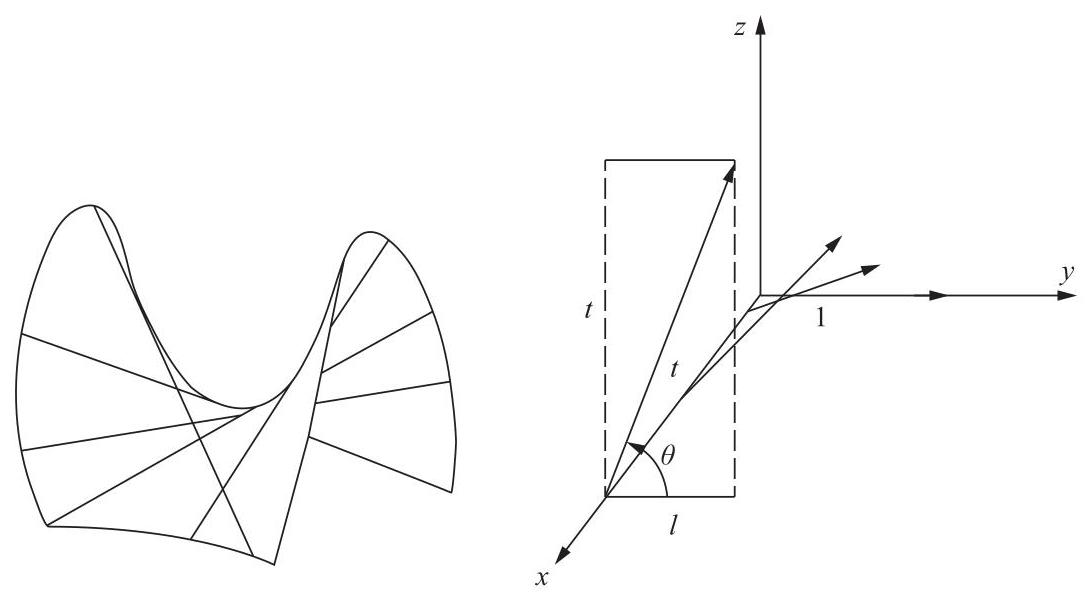
\includegraphics[max width=0.9\textwidth]{images/bo_d4b9jf3ef24c73e0334g_207_220_1001_1092_599_0.jpg}
\end{center}
\hspace*{3em} 

图 3-35. \(z = {xy}\) 作为直纹面.

自 \({\alpha }^{\prime }\left( t\right)  = \left( {1,0,0}\right)\) 起，我们得到切线是 \(\alpha\) 本身.分布参数是

\[
\lambda  = \frac{1}{k}
\]

我们还注意到，角 \(\theta\) 的正切值，该角由 \(w\left( t\right)\) 与 \(w\left( 0\right)\) 所成，是 \(\tan \theta  = {tk}\) .

最后的注记引出了一个有趣的直纹曲面的一般性质.如果我们考虑一个正则直纹曲面的一条生成线上的法向量族，这个族会生成另一个直纹曲面.根据公式 (7) 和最后的注记，后者曲面正是双曲抛物面 \(z = {kxy}\) ，其中 \(1/k\) 是在选定的生成线上分布参数的值.

在直纹曲面中，可展曲面扮演着重要的角色.让我们重新从一个任意的直纹曲面(不一定是圆柱面)开始

\[
\mathbf{x}\left( {t,v}\right)  = \alpha \left( t\right)  + {vw}\left( t\right) , \tag{8}
\]

由族 \(\{ \alpha \left( t\right) ,w\left( t\right) \}\) 和 \(\left| {w\left( t\right) }\right|  \equiv  1\) 生成.曲面 (8) 被称为可展曲面，如果

\[
\left( {w,{w}^{\prime },{\alpha }^{\prime }}\right)  \equiv  0. \tag{9}
\]

为了找到条件 (9) 的几何解释，我们将计算可展曲面在正则点的斯氏曲率.与为得到公式 (6) 所做的计算完全类似，得到

\[
g = 0,\;f = \frac{\left( w,{w}^{\prime },{\alpha }^{\prime }\right) }{\left| {\mathbf{x}}_{t} \land  {\mathbf{x}}_{v}\right| }.
\]

根据条件 (9)， \(f \equiv  0\) ；因此，

\[
K = \frac{{eg} - {f}^{2}}{{EG} - {F}^{2}} \equiv  0.
\]

这意味着，在正则点，可展曲面的斯氏曲率恒等于零.

关于可展曲面的另一种几何解释，请参见练习 6.

我们现在可以区分可展曲面的两种非穷尽情况:

1. \(w\left( t\right)  \land  {w}^{\prime }\left( t\right)  \equiv  0\) .这意味着 \({w}^{\prime }\left( t\right)  \equiv  0\) .因此， \(w\left( t\right)\) 是常数，并且直纹曲面是圆柱面，其母线由圆柱面与垂直于 \(w\left( t\right)\) 的平面相交得到.

2. 对所有 \(t \in  I\) 都有 \(w\left( t\right)  \land  {w}^{\prime }\left( t\right)  \neq  0\) .在这种情况下，对所有 \(t \in  I\) 都有 \({w}^{\prime }\left( t\right)  \neq  0\) .因此，曲面是非圆柱面的，我们可以应用我们之前的工作.因此，我们可以确定切线(2)并检查分布参数

\[
\lambda  = \frac{\left( {\beta }^{\prime },w,{w}^{\prime }\right) }{{\left| {w}^{\prime }\right| }^{2}} \equiv  0. \tag{10}
\]

因此，切线将是可展曲面的奇异点的轨迹.如果对所有 \(t \in  I\) 都有 \({\beta }^{\prime }\left( t\right)  \neq  0\) ，则根据公式 (10) 和 \(\left\langle  {{\beta }^{\prime },{w}^{\prime }}\right\rangle   \equiv  0\) 的事实，可以得出 \(w\) 平行于 \({\beta }^{\prime }\) .因此，直纹曲面是 \(\beta\) 的切面.如果对所有 \(t \in  I\) 都有 \({\beta }^{\prime }\left( t\right)  = 0\) ，则切线是一个点，并且直纹曲面是以该点为顶点的锥面.

当然，上述情况并非穷尽所有可能性.通常，如果所涉及的函数的零点聚集，分析可能会变得相当复杂.无论如何，远离这些聚集点，可展曲面是圆柱面、锥面和切面的组合.

正如我们所见，在正则点，可展曲面的斯氏曲率恒等于零.在第 5-8 节中，我们将证明一个关于此的全局反例，该反例表明一个正则曲面 \(S \subset  {R}^{3}\) ，它作为 \({R}^{3}\) 的子集是闭合的并且斯氏曲率为零，则是一个圆柱面.

示例 4(曲面上曲线的切平面族包络).设 \(S\) 为一个正则曲面， \(\alpha  = \alpha \left( s\right)\) 为 \(S\) 上一条由弧长参数化的曲线.假设 \(\alpha\) 处处不与渐近方向相切.考虑由以下方式定义的直纹曲面

\[
\mathbf{x}\left( {s,v}\right)  = \alpha \left( s\right)  + v\frac{N\left( s\right)  \land  {N}^{\prime }\left( s\right) }{\left| {N}^{\prime }\left( s\right) \right| }, \tag{11}
\]

其中 \(N\left( s\right)\) 表示 \(S\) 在曲线 \(\alpha \left( s\right)\) 上的单位法向量(由于 \({\alpha }^{\prime }\left( s\right)\) 不是渐近方向，因此对所有 \(s\) 都有 \({N}^{\prime }\left( s\right)  \neq  0\) ).我们将证明 \(\mathbf{x}\) 是一个可展曲面，在 \(v = 0\) 的邻域内是正则的，并且沿着 \(v = 0\) 与 \(S\) 相切.但在此之前，让我们给出曲面 \(\mathbf{x}\) 的几何解释.

考虑曲面 \(S\) 沿曲线 \(\alpha \left( s\right)\) 的切平面族 \(\left\{  {{T}_{\alpha \left( s\right) }\left( S\right) }\right\}\) .如果 \({\Delta s}\) 很小，族中的两个平面 \({T}_{\alpha \left( s\right) }\left( S\right)\) 和 \({T}_{\alpha \left( {s + {\Delta s}}\right) }\left( S\right)\) 将沿着一条平行于向量的直线相交

\[
\frac{N\left( s\right)  \land  N\left( {s + {\Delta s}}\right) }{\Delta s}.
\]

如果我们令 \({\Delta s}\) 趋于零，这条直线将趋近于一个平行于向量的极限位置

\[
\mathop{\lim }\limits_{{{\Delta s} \rightarrow  0}}\frac{N\left( s\right)  \land  N\left( {s + {\Delta s}}\right) }{\Delta s} = \mathop{\lim }\limits_{{{\Delta s} \rightarrow  0}}N\left( s\right)  \land  \frac{\left( N\left( s + \Delta s\right)  - N\left( s\right) \right) }{\Delta s}
\]

\[
= N\left( s\right)  \land  {N}^{\prime }\left( s\right) .
\]

直观上，这意味着 \(\mathbf{x}\) 的生成线是族 \(\left\{  {{T}_{\alpha \left( s\right) }\left( S\right) }\right\}\) 的相邻平面交线的极限位置. \(\mathbf{x}\) 被称为 S 沿 \(\alpha \left( S\right)\) 的切平面族的包络(图 3-36).

例如，如果 \(\alpha\) 是球面 \({S}^{2}\) 的平行线参数化，那么 \({S}^{2}\) 沿 \(\alpha\) 的切平面包络是圆柱面(如果平行线是赤道)或圆锥面(如果平行线不是赤道)(图 3-37).

\begin{center}
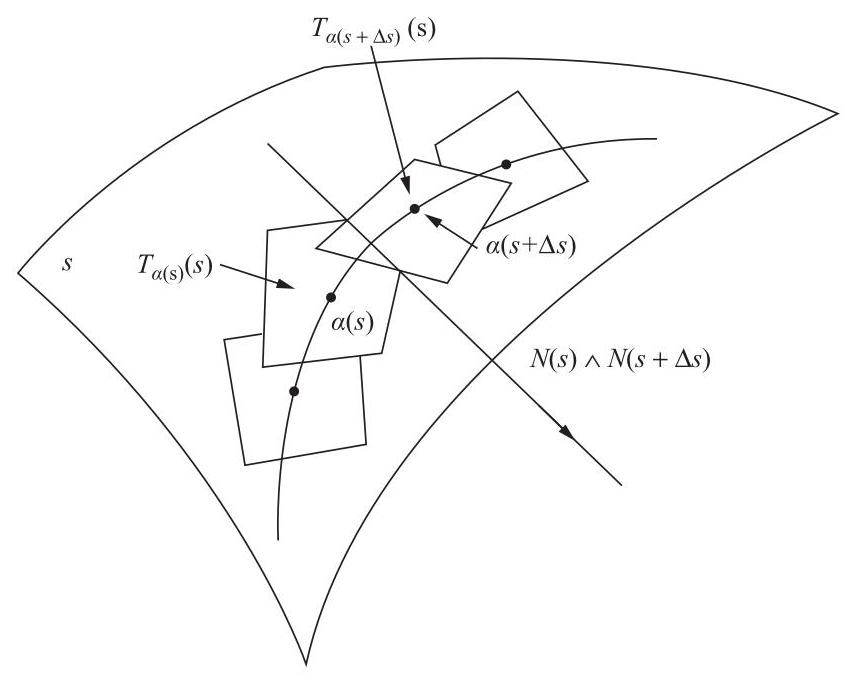
\includegraphics[max width=0.7\textwidth]{images/bo_d4b9jf3ef24c73e0334g_210_356_191_854_676_0.jpg}
\end{center}
\hspace*{3em} 

图 3-36

\begin{center}
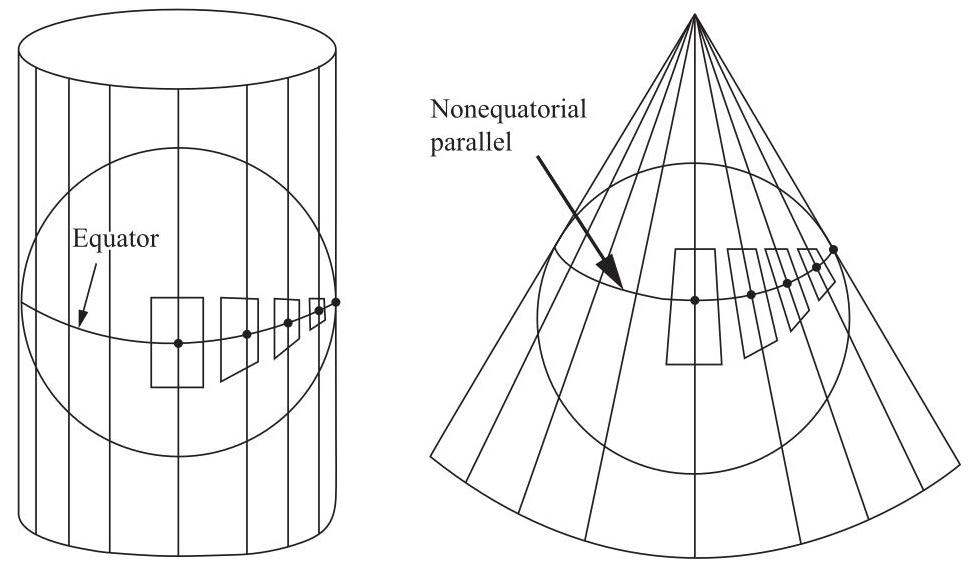
\includegraphics[max width=0.8\textwidth]{images/bo_d4b9jf3ef24c73e0334g_210_295_977_976_564_0.jpg}
\end{center}
\hspace*{3em} 

图 3-37. 球面平行线切平面族包络.

为了证明 \(\mathbf{x}\) 是一个可展曲面，我们将检查条件 (9) 对 \(\mathbf{x}\) 是否成立.事实上，通过直接计算，我们得到

\[
\left\langle  {\frac{N \land  {N}^{\prime }}{\left| {N}^{\prime }\right| } \land  {\left( \frac{N \land  {N}^{\prime }}{\left| {N}^{\prime }\right| }\right) }^{\prime },{\alpha }^{\prime }}\right\rangle   = \left\langle  {\frac{N \land  {N}^{\prime }}{\left| {N}^{\prime }\right| } \land  \frac{{\left( N \land  {N}^{\prime }\right) }^{\prime }}{\left| {N}^{\prime }\right| },{\alpha }^{\prime }}\right\rangle
\]

\[
= \frac{1}{{\left| {N}^{\prime }\right| }^{2}}\left\langle  {\left\langle  {N \land  {N}^{\prime },{N}^{\prime \prime }}\right\rangle  N,{\alpha }^{\prime }}\right\rangle   = 0.
\]

这就证明了我们的主张.

现在我们将证明 \(\mathbf{x}\) 在 \(v = 0\) 的邻域内是正则的，并且它沿着 \(\alpha\) 与 \(S\) 相切.事实上，在 \(v = 0\) 处，我们有

\[
{\mathbf{x}}_{s} \land  {\mathbf{x}}_{v} = {\alpha }^{\prime } \land  \frac{\left( N \land  {N}^{\prime }\right) }{\left| {N}^{\prime }\right| } = \left\langle  {{N}^{\prime },{\alpha }^{\prime }}\right\rangle  \frac{N}{\left| {N}^{\prime }\right| } =  - \left\langle  {N,{\alpha }^{\prime \prime }}\right\rangle  \frac{N}{\left| {N}^{\prime }\right| }
\]

\[
=  - \frac{\left( {k}_{n}N\right) }{\left| {N}^{\prime }\right| },
\]

其中 \({k}_{n} = {k}_{n}\left( s\right)\) 是 \(\alpha\) 的法曲率.由于 \({k}_{n}\left( s\right)\) 处处不为零，这表明 \(\mathbf{x}\) 在 \(v = 0\) 的邻域内是正则的，并且 \(\mathbf{x}\) 在 \(\mathbf{x}\left( {s,0}\right)\) 处的单位法向量与 \(N\left( s\right)\) 一致.因此， \(\mathbf{x}\) 沿着 \(v = 0\) 与 \(S\) 相切，这就完成了我们断言的证明.

我们将总结我们的结论如下.设 \(\alpha \left( s\right)\) 是曲面 \(S\) 上一条由弧长参数化的曲线，并假设 \(\alpha\) 处处不与渐近方向相切.那么 \(S\) 沿 \(\alpha\) 的切平面族的包络 (11) 是一个可展曲面，在 \(\alpha \left( s\right)\) 的邻域内是正则的，并且沿着 \(\alpha \left( s\right)\) 与 \(S\) 相切.

\section*{B. 极小曲面}

一个正则参数化曲面称为极小曲面，如果它的平均曲率处处为零.一个正则曲面 \(S \subset  {R}^{3}\) 是极小曲面，如果它的每一个参数化都是极小的.

为了解释为什么我们对这样的曲面使用“极小”一词，我们需要引入“变分”的概念.设 \(\mathbf{x} : U \subset  {R}^{2} \rightarrow  {R}^{3}\) 为一个正则参数化曲面.选择一个有界区域 \(D \subset  U\) (参见第 2-5 节) 和一个可微函数 \(h : \bar{D} \rightarrow  R\) ，其中 \(\bar{D}\) 是区域 \(D\) 与其边界 \(\partial D\) 的并集.由 \(h\) 确定的 \(\mathbf{x}\left( \bar{D}\right)\) 的法向变分是如图 3-38 所示的映射，该映射由下式给出:

\[
\varphi  : \bar{D} \times  \left( {-\epsilon ,\epsilon }\right)  \rightarrow  {R}^{3}
\]

\[
\varphi \left( {u,v,t}\right)  = \mathbf{x}\left( {u,v}\right)  + {th}\left( {u,v}\right) N\left( {u,v}\right) ,\;\left( {u,v}\right)  \in  \bar{D},t \in  \left( {-\epsilon ,\epsilon }\right) .
\]

对于每个固定的 \(t \in  \left( {-\epsilon ,\epsilon }\right)\) ，映射 \({\mathbf{x}}^{t} : D \rightarrow  {R}^{3}\)

\[
{\mathbf{x}}^{\prime }\left( {u,v}\right)  = \varphi \left( {u,v,t}\right)
\]

是一个参数化曲面，具有

\[
\frac{\partial {\mathbf{x}}^{t}}{\partial u} = {\mathbf{x}}_{u} + {th}{N}_{u} + t{h}_{u}N
\]

\[
\frac{\partial {\mathbf{x}}^{t}}{\partial v} = {\mathbf{x}}_{v} + {th}{N}_{v} + t{h}_{v}N
\]

\begin{center}
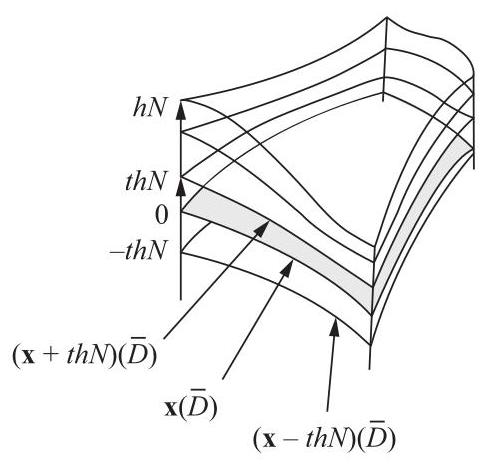
\includegraphics[max width=0.4\textwidth]{images/bo_d4b9jf3ef24c73e0334g_212_201_188_487_468_0.jpg}
\end{center}
\hspace*{3em} 

图 3-38. \(\mathbf{x}\left( D\right)\) 的法向变分.

因此，如果我们用 \({E}^{t},{F}^{t},{G}^{t}\) 表示 \({\mathbf{x}}^{t}\) 的第一基本形式的系数，我们得到

\[
{E}^{t} = E + {th}\left( {\left\langle  {{\mathbf{x}}_{u},{N}_{u}}\right\rangle   + \left\langle  {{\mathbf{x}}_{u},{N}_{u}}\right\rangle  }\right)  + {t}^{2}{h}^{2}\left\langle  {{N}_{u},{N}_{u}}\right\rangle   + {t}^{2}{h}_{u}{h}_{u},
\]

\[
{F}^{t} = F + {th}\left( {\left\langle  {{\mathbf{x}}_{u},{N}_{v}}\right\rangle   + \left\langle  {{\mathbf{x}}_{v},{N}_{u}}\right\rangle  }\right)  + {t}^{2}{h}^{2}\left\langle  {{N}_{u},{N}_{v}}\right\rangle   + {t}^{2}{h}_{u}{h}_{v},
\]

\[
{G}^{t} = G + {th}\left( {\left\langle  {{\mathbf{x}}_{v},{N}_{v}}\right\rangle   + \left\langle  {{\mathbf{x}}_{v},{N}_{v}}\right\rangle  }\right)  + {t}^{2}{h}^{2}\left\langle  {{N}_{v},{N}_{v}}\right\rangle   + {t}^{2}{h}_{v}{h}_{v}.
\]

利用以下事实:

\[
\left\langle  {{\mathbf{x}}_{u},{N}_{u}}\right\rangle   =  - e,\;\left\langle  {{\mathbf{x}}_{u},{N}_{v}}\right\rangle   + \left\langle  {{\mathbf{x}}_{v},{N}_{u}}\right\rangle   =  - {2f},\;\left\langle  {{\mathbf{x}}_{v},{N}_{v}}\right\rangle   =  - g
\]

并且平均曲率 \(H\) 为 (参见第 3-3 节，方程 (5))

\[
H = \frac{1}{2}\frac{{Eg} - {2fF} + {Ge}}{{EG} - {F}^{2}},
\]

我们得到

\[
{E}^{t}{G}^{t} - {\left( {F}^{\prime }\right) }^{2} = {EG} - {F}^{2} - {2th}\left( {{Eg} - {2FJ} + {Ge}}\right)  + R
\]

\[
= \left( {{EG} - {F}^{2}}\right) \left( {1 - {4thH}}\right)  + R,
\]

其中 \(\mathop{\lim }\limits_{{t \rightarrow  0}}\left( {R/t}\right)  = 0\) .

由此可知，如果 \(\epsilon\) 足够小， \({\mathbf{x}}^{t}\) 是一个正则参数化曲面.此外， \({\mathbf{x}}^{t}\left( \bar{D}\right)\) 的面积 \(A\left( t\right)\) 为

\[
A\left( t\right)  = {\int }_{\bar{D}}\sqrt{{E}^{t}{G}^{t} - {\left( {F}^{t}\right) }^{2}}{dudv}
\]

\[
= {\int }_{\bar{D}}\sqrt{1 - {4thH} + \bar{R}}\sqrt{{EG} - {F}^{2}}{dudv},
\]

其中 \(\bar{R} = R/\left( {{EG} - {F}^{2}}\right)\) .由此可知，如果 \(\epsilon\) 很小， \(A\) 是一个可微函数，并且它在 \(t = 0\) 处的导数为

\[
{A}^{\prime }\left( 0\right)  =  - {\int }_{\bar{D}}{2hH}\sqrt{{EG} - {F}^{2}}{dudv} \tag{12}
\]

现在我们准备好解释为什么在平均曲率为零的曲面中使用“极小”一词了.

命题 1. 设 \(x : \mathrm{U} \rightarrow  {\mathbb{R}}^{3}\) 为一个正则参数化曲面，设 \(\mathrm{D} \subset  \mathrm{U}\) 为 \(\mathrm{U}\) 中的一个有界区域.则 \(\mathbf{x}\) 是极小的，当且仅当对于所有这样的 \(\mathrm{D}\) 和所有 \(\mathbf{x}\left( \bar{D}\right)\) 的法向变分，都有 \({\mathrm{A}}^{\prime }\left( 0\right)  = 0\) .

证明. 如果 \(\mathbf{x}\) 是极小的，则 \(H \equiv  0\) ，并且该条件显然满足.反之，假设条件满足，并且对于某个 \(q \in  D\) ，有 \(H\left( q\right)  \neq  0\) .选择 \(h : \bar{D} \rightarrow  R\) 使得 \(h\left( q\right)  = H\left( q\right) ,{hH} > 0\) ，并且 \(h\) 在 \(q\) 的一个小邻域外部处处为零.则对于由该 \(h\) 确定的变分，有 \({A}^{\prime }\left( 0\right)  < 0\) ，这是一个矛盾.Q.E.D.

因此，极小曲面 \(\mathbf{x}\) 的任何有界区域 \(\mathbf{x}\left( \bar{D}\right)\) 对于任何 \(\mathbf{x}\left( \bar{D}\right)\) 的法向变分的面积函数来说都是一个临界点.应该注意到，这个临界点可能不是最小值，这使得“极小”一词显得有些不恰当.然而，这是一个历史悠久的术语，由拉格朗日 (他首先定义了极小曲面) 于 1760 年引入.

极小曲面通常与肥皂膜相关，肥皂膜可以通过将金属丝框浸入肥皂溶液中然后小心取出而获得.如果实验进行得好，得到的肥皂膜将具有与框架相同的边界.通过物理考虑可以证明，肥皂膜会处于一个位置，在该位置的规则点上，平均曲率为零.通过这种方式，我们可以“制造”出美丽的极小曲面，例如图 3-39 中的那个.

\begin{center}
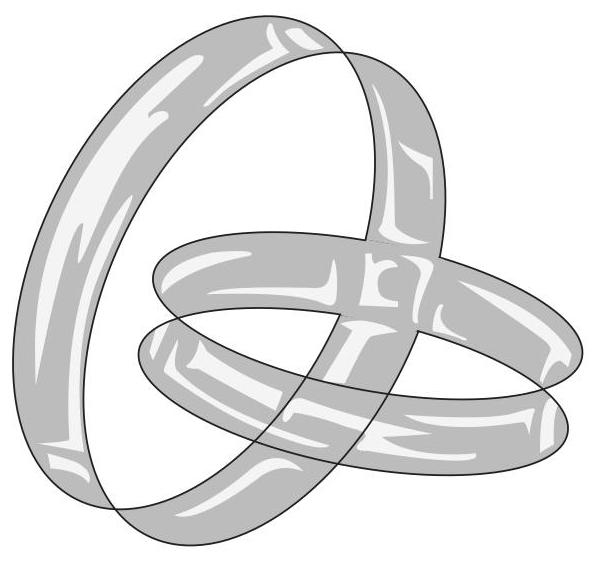
\includegraphics[max width=0.5\textwidth]{images/bo_d4b9jf3ef24c73e0334g_213_180_1290_596_563_0.jpg}
\end{center}
\hspace*{3em} 

图 3-39

注 1. 应该指出的是，并非所有肥皂膜都符合我们定义的极小曲面.我们假设极小曲面是规则的(我们可以假设存在一些孤立的奇异点，但超出这一点将使处理过程不那么基础).然而，肥皂

\begin{center}
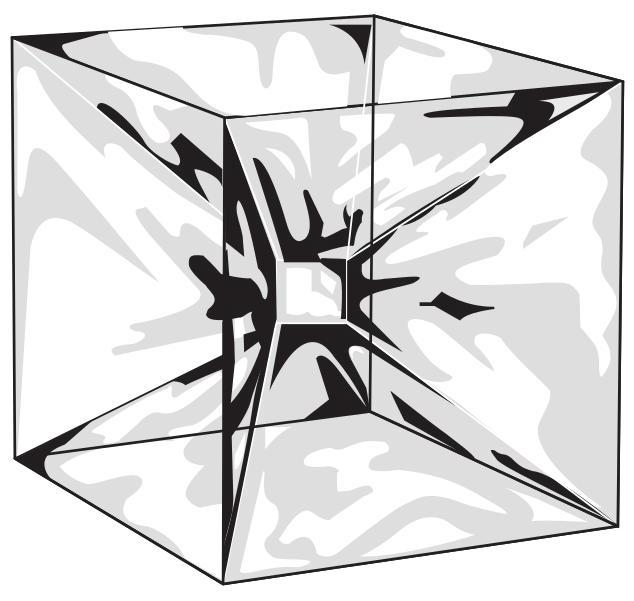
\includegraphics[max width=0.5\textwidth]{images/bo_d4b9jf3ef24c73e0334g_214_200_192_634_601_0.jpg}
\end{center}
\hspace*{3em} 

图 3-40

膜可以通过例如使用立方体作为框架(图 3-40)形成，该框架沿线具有奇异点.

注 2. 极小曲面与肥皂膜之间的联系启发了著名的普拉托问题(普拉托是比利时物理学家，他在 1850 年左右对肥皂膜进行了仔细的实验).该问题可以大致描述如下:证明对于每个闭合曲线 \(\mathrm{C} \subset  {\mathbb{R}}^{3}\) 都存在一个面积最小的曲面 \(S\) ，其边界为 \(\mathrm{C}\) .使问题精确化(允许哪些曲线和曲面，以及 \(C\) 是 \(S\) 的边界意味着什么)本身就是问题的一个非平凡部分.普拉托问题的一个版本于 1930 年由 Douglas 和 Radó 同时解决.其他版本(以及更高维问题的推广)激发了数学实体的创建，这些实体至少包含了与肥皂状薄膜一样多的东西.有关普拉托问题的更多细节和最新参考文献，请参阅本书末尾的 Lawson [20] 的第 2 章.

为了方便起见，我们将为任意参数化的规则曲面引入由 \(\mathbf{H} = {HN}\) 定义的平均曲率向量. \(\mathbf{H}\) 方向的几何意义可以从方程 (12) 中获得.事实上，如果我们选择 \(h = H\) ，对于这个特定的变分，我们有，

\[
{A}^{\prime }\left( 0\right)  =  - 2{\int }_{\bar{D}}\langle \mathbf{H},\mathbf{H}\rangle \sqrt{{EG} - {F}^{2}}{dudv} < 0.
\]

这意味着如果我们沿着向量 \(\mathbf{H}\) 的方向变形 \(\mathbf{x}\left( \overline{\mathrm{D}}\right)\) ，面积最初会减小.

平均曲率向量还有另一种解释，我们将继续探讨，因为它对极小曲面理论有重要意义.

一个规则参数化曲面 \(\mathbf{x} = \mathbf{x}\left( {u,v}\right)\) 被称为等温的，如果 \(\left\langle  {{\mathbf{x}}_{u},{\mathbf{x}}_{u}}\right\rangle   = \left\langle  {{\mathbf{x}}_{v},{\mathbf{x}}_{v}}\right\rangle\) 和 \(\left\langle  {{\mathbf{x}}_{u},{\mathbf{x}}_{v}}\right\rangle   = 0\) .

命题 2. 令 \(\mathbf{x} = \mathbf{x}\left( {\mathrm{u},\mathrm{v}}\right)\) 为一个规则参数化曲面，并假设 \(\mathbf{x}\) 是等温的.则

\[
{\mathbf{x}}_{\mathrm{{uu}}} + {\mathbf{x}}_{\mathrm{{vv}}} = 2{\lambda }^{2}\mathbf{H},
\]

其中 \({\lambda }^{2} = \left\langle  {{\mathbf{x}}_{\mathrm{u}},{\mathbf{x}}_{\mathrm{u}}}\right\rangle   = \left\langle  {{\mathbf{x}}_{\mathrm{v}},{\mathbf{x}}_{\mathrm{v}}}\right\rangle\) .

证明.由于 \(\mathbf{x}\) 是等温的， \(\left\langle  {{\mathbf{x}}_{u},{\mathbf{x}}_{u}}\right\rangle   = \left\langle  {{\mathbf{x}}_{v},{\mathbf{x}}_{v}}\right\rangle\) 和 \(\left\langle  {{\mathbf{x}}_{u},{\mathbf{x}}_{v}}\right\rangle   = 0\) .通过微分，我们得到

\[
\left\langle  {{\mathbf{x}}_{uu},{\mathbf{x}}_{u}}\right\rangle   = \left\langle  {{\mathbf{x}}_{vu},{\mathbf{x}}_{v}}\right\rangle   =  - \left\langle  {{\mathbf{x}}_{u},{\mathbf{x}}_{vv}}\right\rangle  .
\]

因此，

\[
\left\langle  {{\mathbf{x}}_{uu} + {\mathbf{x}}_{vv},{\mathbf{x}}_{u}}\right\rangle   = 0.
\]

类似地，

\[
\left\langle  {{\mathbf{x}}_{uu} + {\mathbf{x}}_{vv},{\mathbf{x}}_{v}}\right\rangle   = 0.
\]

由此可知 \({\mathbf{x}}_{uu} + {\mathbf{x}}_{vv}\) 平行于 \(N\) .由于 \(\mathbf{x}\) 是等温的，

\[
H = \frac{1}{2}\frac{g + e}{{\lambda }^{2}}.
\]

因此，

\[
2{\lambda }^{2}H = g + e = \left\langle  {N,{\mathbf{x}}_{uu} + {\mathbf{x}}_{vv}}\right\rangle  ;
\]

因此，

\[
{\mathbf{x}}_{uu} + {\mathbf{x}}_{vv} = 2{\lambda }^{2}\mathbf{H}. \tag{Q.E.D.}
\]

可微函数 \(f : U \subset  {R}^{2} \rightarrow  R\) 的拉普拉斯算子 \({\Delta f}\) 定义为 \({\Delta f} = \left( {{\partial }^{2}f/\partial {u}^{2}}\right)  + \left( {{\partial }^{2}f/\partial {v}^{2}}\right) ,\left( {u,v}\right)  \in  U\) .如果 \({\Delta f} = 0\) ，则称 \(f\) 在 \(U\) 中是调和的.从命题 2，我们得到

推论:设 \(x\left( {\mathrm{u},\mathrm{v}}\right)  = \left( {x\left( {\mathrm{u},\mathrm{v}}\right) ,\mathrm{y}\left( {\mathrm{u},\mathrm{v}}\right) ,\mathrm{z}\left( {\mathrm{u},\mathrm{v}}\right) }\right)\) 为一个参数化曲面，并假设 \(\mathbf{x}\) 是等温的.则 \(\mathbf{x}\) 是极小的，当且仅当其坐标函数 \(x,\mathrm{y},\mathrm{z}\) 是调和的.

例 5. 悬链面，由下式给出

\[
\mathbf{x}\left( {u,v}\right)  = \left( {a\cosh v\cos u,a\cosh v\sin u,{av}}\right) ,
\]

\[
0 < u < {2\pi },\; - \infty  < v < \infty .
\]

这是由将悬链线 \(y = a\cosh \left( {z/a}\right)\) 绕 \(z\) 轴旋转生成的曲面(图 3-41).很容易验证 \(E = G = {a}^{2}{\cosh }^{2}v,F = 0\) ，并且 \({\mathbf{x}}_{uu} + {\mathbf{x}}_{vv} = 0\) .因此，悬链面是极小曲面.它可以被表征为唯一极小的旋转曲面.

\begin{center}
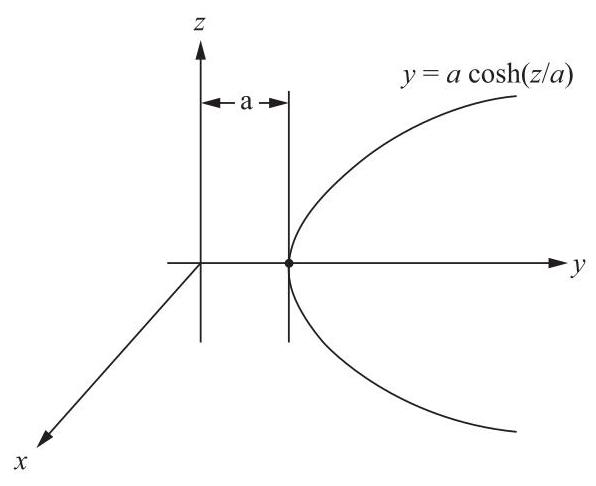
\includegraphics[max width=0.5\textwidth]{images/bo_d4b9jf3ef24c73e0334g_216_195_198_596_486_0.jpg}
\end{center}
\hspace*{3em} 

图 3-41

最后的论断可以如下证明.我们想找到一条曲线 \(y = \; f\left( x\right)\) ，当它绕 \(x\) 轴旋转时，会描述一个极小曲面.由于旋转曲面的平行线和经线是曲面的曲率线(第 3-3 节，例 4)，我们必须有曲线 \(y = f\left( x\right)\) 的曲率等于由点 \(f\left( x\right)\) 生成的圆的法曲率的负值(两者都是主曲率).由于 \(y = f\left( x\right)\) 的曲率为

\[
\frac{{y}^{\prime \prime }}{{\left( 1 + {\left( {y}^{\prime }\right) }^{2}\right) }^{3/2}}
\]

而圆的法曲率为其通常曲率 \(\left( { = 1/y}\right)\) 在曲面法向量 \(N\) 上的投影(见图 3-42)，我们得到

\[
\frac{{y}^{\prime \prime }}{{\left( 1 + {\left( {y}^{\prime }\right) }^{2}\right) }^{3/2}} =  - \frac{1}{y}\cos \varphi .
\]

但是 \(- \cos \varphi  = \cos \theta\) (见图 3-42)，并且由于 \(\tan \theta  = {y}^{\prime }\) ，我们得到

\[
\frac{{y}^{\prime \prime }}{{\left( 1 + {\left( {y}^{\prime }\right) }^{2}\right) }^{3/2}} = \frac{1}{y}\frac{1}{{\left( 1 + {\left( {y}^{\prime }\right) }^{2}\right) }^{1/2}}
\]

\begin{center}
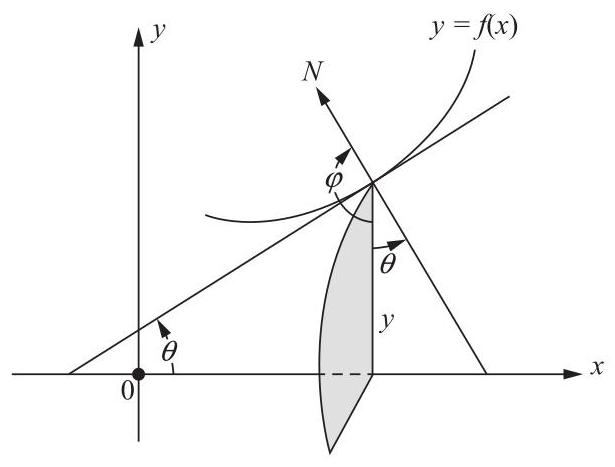
\includegraphics[max width=0.5\textwidth]{images/bo_d4b9jf3ef24c73e0334g_216_197_1645_615_467_0.jpg}
\end{center}
\hspace*{3em} 

图 3-42

作为曲线 \(y = f\left( x\right)\) 需要满足的方程.

显然，存在一点 \(x\) ，使得 \({f}^{\prime }\left( x\right)  \neq  0\) .让我们在该点附近工作，其中 \({f}^{\prime } \neq  0\) .将上述方程的两边乘以 \(2{y}^{\prime }\) ，我们得到，

\[
\frac{2{y}^{\prime \prime }{y}^{\prime }}{1 + {\left( {y}^{\prime }\right) }^{2}} = \frac{2{y}^{\prime }}{y}.
\]

令 \(1 + {\left( {y}^{\prime }\right) }^{2} = z\) (因此， \(2{y}^{\prime \prime }{y}^{\prime } = {z}^{\prime }\) )，我们得到

\[
\frac{{z}^{\prime }}{z} = \frac{2{y}^{\prime }}{y}
\]

通过积分，得到 \(\left( {k\text{ is a constant }}\right)\)

\[
\log z = \log {y}^{2} + \log {k}^{2} = \log {\left( yk\right) }^{2}
\]

or

\[
1 + {\left( {y}^{\prime }\right) }^{2} = z = {\left( yk\right) }^{2}.
\]

最后的表达式可以写成

\[
\frac{kdy}{\sqrt{{\left( yk\right) }^{2} - 1}} = {kdx}
\]

通过积分再次得到( \(c\) 是一个常数)

\[
{\cosh }^{-1}\left( {yk}\right)  = {kx} + c
\]

or

\[
y = \frac{1}{k}\cosh \left( {{kx} + c}\right) .
\]

因此，在 \({f}^{\prime } \neq  0\) 处的点附近，曲线 \(y = f\left( x\right)\) 是悬链线.但 \({y}^{\prime }\) 只能在 \(x = 0\) 处为零，如果曲面是连通的，那么它通过连续性成为悬链面，正如我们所声称的.

例 6(螺旋面).(参见第 2-5 节的例 3.)

\[
\mathbf{x}\left( {u,v}\right)  = \left( {a\sinh v\cos u,a\sinh v\sin u,{au}}\right) .
\]

很容易验证 \(E = G = {a}^{2}{\cosh }^{2}v,F = 0\) 和 \({\mathbf{x}}_{uu} + {\mathbf{x}}_{vv} = 0\) .因此，螺旋面是一个极小曲面.它还有一个额外的性质，即除了平面之外，它是唯一一个也是一个直纹曲面的极小曲面.

如果我们假设极小曲面的高斯曲率为零的点是孤立的(证明参见奥斯曼在本文末尾引用的调查，第 76 页)，我们可以给出最后一个断言的证明.有了这个假设，我们将按如下方式进行.

假设曲面不是平面.那么在曲面的某个邻域 \(W\) 中，高斯曲率 \(K\) 严格为负.由于平均曲率为零， \(W\) 被两个相互正交的渐近线族覆盖.由于直纹线是渐近线，并且曲面不是平面，我们可以选择一个点 \(q \in  W\) ，使得除了通过 \(q\) 的直纹线之外的渐近线在 \(q\) 处具有非零的挠率 \(\tau  = \sqrt{-K}\) .由于渐近线的密切平面是曲面的切平面，存在一个邻域 \(V \subset  W\) ，使得 \(V\) 的直纹线是扭曲渐近线族的法线(图 3-43).这是一个关于曲线的有趣练习，可以证明这种情况仅当扭曲曲线是圆柱螺旋线时发生(参见第 1-5 节的练习 18).因此， \(V\) 是螺旋面的一部分.由于圆柱螺旋线的挠率是常数，我们很容易看出整个曲面是螺旋面的一部分，正如我们所声称的.

螺旋面和悬链面由 Meusnier 于 1776 年发现，他还证明了拉格朗日关于极小曲面作为变分问题的临界点的定义等同于平均曲率为零.很长一段时间以来，它们是唯一已知的极小曲面例子.直到 1835 年 Scherk 才找到更多的例子，其中一个在例 8 中进行了描述.在练习 14 中，我们将描述螺旋面和悬链面之间的一个有趣联系.

\begin{center}
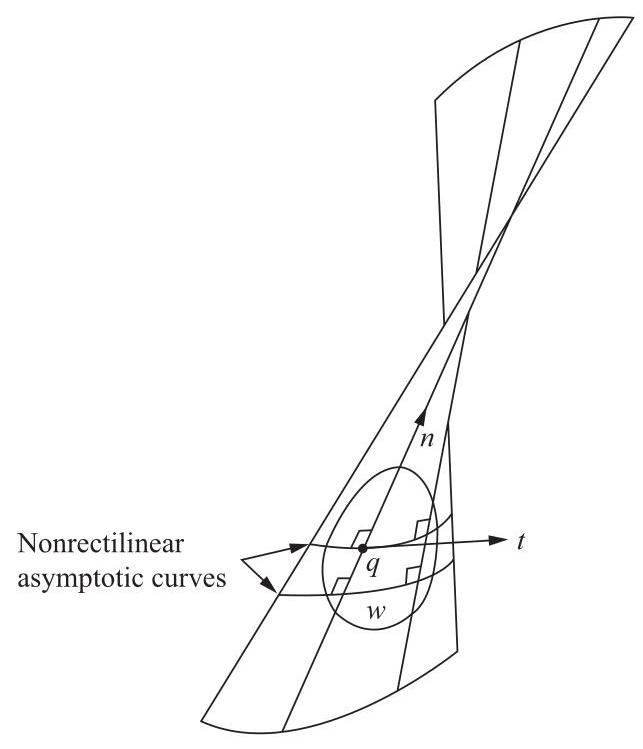
\includegraphics[max width=0.5\textwidth]{images/bo_d4b9jf3ef24c73e0334g_218_192_1366_643_749_0.jpg}
\end{center}
\hspace*{3em} 

图 3-43

例 7(Enneper 极小曲面).Enneper 曲面是参数化曲面

\[
\mathbf{x}\left( {u,v}\right)  = \left( {u - \frac{{u}^{3}}{3} + u{v}^{2},v - \frac{{v}^{3}}{3} + v{u}^{2},{u}^{2} - {v}^{2}}\right) ,\;\left( {u,v}\right)  \in  {R}^{2},
\]

很容易看出它是极小的(图 3-44).请注意，通过将 \(\left( {u,v}\right)\) 变为 \(\left( {-v,u}\right)\) ，我们在曲面中将 \(\left( {x,y,z}\right)\) 变为 \(\left( {-y,x, - z}\right)\) .因此，如果我们绕 \(z\) 轴进行 \(\pi /2\) 的正向旋转，然后进行 \({xy}\) 平面的对称变换，曲面保持不变.

Enneper 曲面一个有趣的特征是它具有自交点.这可以通过令 \(u = \rho \cos \theta ,v = \rho \sin \theta\) 并写出

\[
\mathbf{x}\left( {\rho ,\theta }\right)  = \left( {\rho \cos \theta  - \frac{{\rho }^{3}}{3}\cos {3\theta },\rho \sin \theta  + \frac{{\rho }^{3}}{3}\sin {3\theta },{\rho }^{2}\cos {2\theta }}\right) .
\]

因此，如果 \(\mathbf{x}\left( {{\rho }_{1},{\theta }_{1}}\right)  = \mathbf{x}\left( {{\rho }_{2},{\theta }_{2}}\right)\) ，直接计算表明

\[
{x}^{2} + {y}^{2} = {\rho }_{1}^{2} + \frac{{\rho }_{1}^{6}}{9} - \cos 4{\theta }_{1}\frac{2{\rho }_{1}^{4}}{3}
\]

\[
= {\left( {\rho }_{1} + \frac{{\rho }_{1}^{3}}{3}\right) }^{2} - \frac{4}{3}{\left( {\rho }_{1}^{2}\cos 2{\theta }_{1}\right) }^{2}
\]

\[
= {\left( {\rho }_{2} + \frac{{\rho }_{2}^{3}}{3}\right) }^{2} - \frac{4}{3}{\left( {\rho }_{2}^{2}\cos 2{\theta }_{2}\right) }^{2}.
\]

\begin{center}
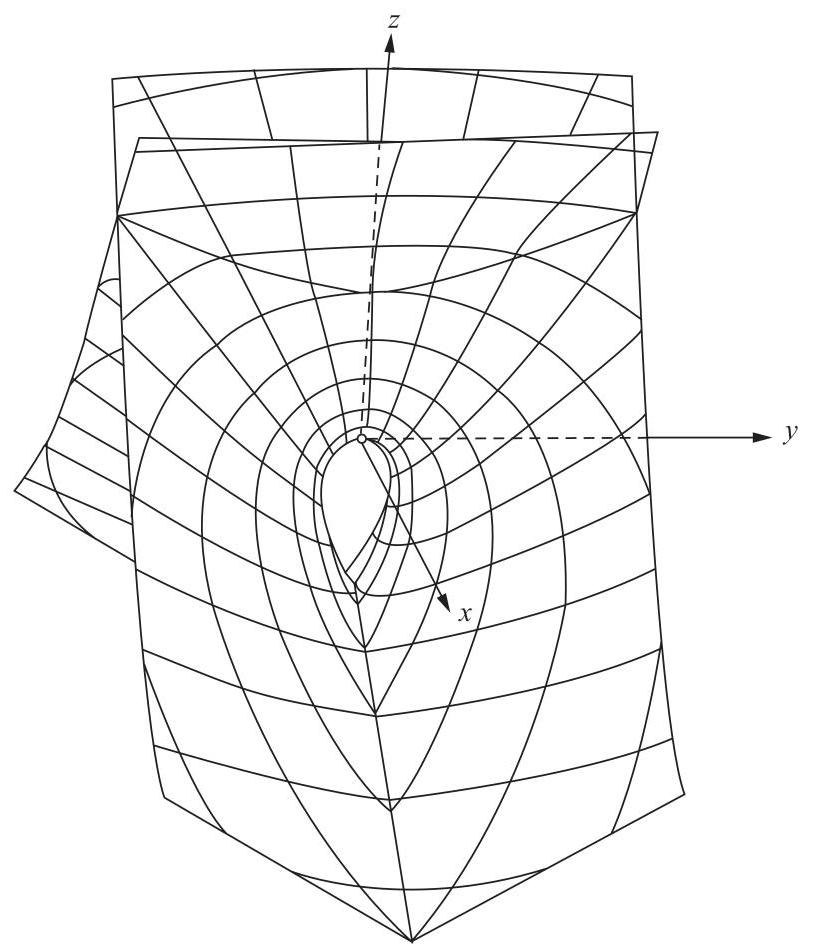
\includegraphics[max width=0.7\textwidth]{images/bo_d4b9jf3ef24c73e0334g_219_361_1000_816_951_0.jpg}
\end{center}
\hspace*{3em} 

图 3-44.Enneper 曲面.经许可，从 K. Leichtweiss 的“Minimalflächen im Grossen，”Überblicke Math. 2 (1969)，7-49，图 4 中修改后转载.

因此，自 \({\rho }_{1}^{2}\cos 2{\theta }_{1} = {\rho }_{2}^{2}\cos 2{\theta }_{2}\) 起，我们得到

\[
{\rho }_{1} + \frac{{\rho }_{1}^{3}}{3} = {\rho }_{2} + \frac{{\rho }_{2}^{3}}{3}
\]

这意味着 \({\rho }_{1} = {\rho }_{2}\) .由此得出 \(\cos 2{\theta }_{1} = \cos 2{\theta }_{2}\) .

例如，如果 \({\rho }_{1} = {\rho }_{2}\) 和 \({\theta }_{1} = {2\pi } - {\theta }_{2}\) ，我们从

\[
y\left( {{\rho }_{1},{\theta }_{1}}\right)  = y\left( {{\rho }_{2},{\theta }_{2}}\right)
\]

得到 \(y =  - y\) .因此， \(y = 0\) ；也就是说，点 \(\left( {{\rho }_{1},{\theta }_{1}}\right)\) 和 \(\left( {{\rho }_{2},{\theta }_{2}}\right)\) 属于曲线 \(\sin \theta  + \left( {{\rho }^{2}/3}\right) \sin {3\theta } = 0\) .显然，对于属于该曲线的每个点 \(\left( {\rho ,\theta }\right)\) ，点 \(\left( {\rho ,{2\pi } - \theta }\right)\) 也属于该曲线，并且

\[
x\left( {\rho ,\theta }\right)  = x\left( {\rho ,{2\pi } - \theta }\right) ,z\left( {\rho ,\theta }\right)  = z\left( {\rho ,{2\pi } - \theta }\right) .
\]

因此，曲面与平面 \(y = 0\) 的交线是曲面自身相交的曲线.

类似地，可以证明曲面与平面 \(x = 0\) 的交线也是自相交曲线(这对应于情况 \(\left. {{\rho }_{1} = {\rho }_{2},{\theta }_{1} = \pi  - {\theta }_{2}}\right)\) .很容易看出它们是 Enneper 曲面的唯一自交线.

我要感谢 Alcides Lins Neto 为绘制图 3-44 的第一张草图而进行的这项工作.

在进入下一个例子之前，我们将建立极小曲面与复变量解析函数之间的一个有用关系.设 \(\mathbb{C}\) 表示复平面，和往常一样，通过令 \(\zeta  = u + {iv},\zeta  \in  \mathbb{C},\left( {u,v}\right)  \in  {R}^{2}\) ，它与 \({R}^{2}\) 等同.我们回顾一下，当把函数 \(f : U \subset  \mathbb{C} \rightarrow  \mathbb{C}\) 写成

\[
f\left( \zeta \right)  = {f}_{1}\left( {u,v}\right)  + i{f}_{2}\left( {u,v}\right) ,
\]

实函数 \({f}_{1}\) 和 \({f}_{2}\) 具有连续的一阶偏导数，并且满足所谓的 Cauchy-Riemann 方程:

\[
\frac{\partial {f}_{1}}{\partial u} = \frac{\partial {f}_{2}}{\partial v},\;\frac{\partial {f}_{1}}{\partial v} =  - \frac{\partial {f}_{2}}{\partial u}.
\]

现在令 \(\mathbf{x} : U \subset  {R}^{2} \rightarrow  {R}^{3}\) 为正则参数化曲面，并定义复函数 \({\varphi }_{1},{\varphi }_{2},{\varphi }_{3}\) 为

\[
{\varphi }_{1}\left( \zeta \right)  = \frac{\partial x}{\partial u} - i\frac{\partial x}{\partial v},\;{\varphi }_{2}\left( \zeta \right)  = \frac{\partial y}{\partial u} - i\frac{\partial y}{\partial v},\;{\varphi }_{3}\left( \zeta \right)  = \frac{\partial z}{\partial u} - i\frac{\partial z}{\partial v},
\]

其中 \(x,y\) ，以及 \(z\) 是 \(\mathbf{x}\) 的分量函数.

引理. \(x\) 是等温的当且仅当 \({\varphi }_{1}^{2} + {\varphi }_{2}^{2} + {\varphi }_{3}^{2} \equiv  0\) .如果满足最后一个条件， \(\mathbf{x}\) 是最小的当且仅当 \({\varphi }_{1},{\varphi }_{2}\) 和 \({\varphi }_{3}\) 是解析函数.

证明.通过简单的计算，我们得到

\[
{\varphi }_{1}^{2} + {\varphi }_{2}^{2} + {\varphi }_{3}^{2} = E - G + {2iF},
\]

因此引理的第一部分.此外， \({\mathbf{x}}_{uu} + {\mathbf{x}}_{vv} = 0\) 当且仅当

\[
\frac{\partial }{\partial u}\left( \frac{\partial x}{\partial u}\right)  =  - \frac{\partial }{\partial v}\left( \frac{\partial x}{\partial v}\right)
\]

\[
\frac{\partial }{\partial u}\left( \frac{\partial y}{\partial u}\right)  =  - \frac{\partial }{\partial v}\left( \frac{\partial y}{\partial v}\right)
\]

\[
\frac{\partial }{\partial u}\left( \frac{\partial z}{\partial u}\right)  =  - \frac{\partial }{\partial v}\left( \frac{\partial z}{\partial v}\right)
\]

这给出了 \({\varphi }_{1},{\varphi }_{2},{\varphi }_{3}\) 的 Cauchy-Riemann 方程的一半.由于另一半自动满足，我们得出结论 \({\mathbf{x}}_{uu} + {\mathbf{x}}_{vv} = 0\) 当且仅当 \({\varphi }_{1},{\varphi }_{2}\) 和 \({\varphi }_{3}\) 是解析的.Q.E.D.

例 8(Scherk 最小曲面).该曲面由下式给出

\[
\mathbf{x}\left( {u,v}\right)  = \left( {\arg \frac{\zeta  + i}{\zeta  - i},\arg \frac{\zeta  + 1}{\zeta  - 1},\log \left| \frac{{\zeta }^{2} + 1}{{\zeta }^{2} - 1}\right| }\right) ,
\]

\[
\zeta  \neq   \pm  1,\zeta  \neq   \pm  i
\]

其中 \(\zeta  = u + {iv}\) ，以及参数 \(\zeta\) 是实轴与 \(\zeta\) 所成的角度.

我们容易计算出

\[
\arg \frac{\zeta  + i}{\zeta  - i} = {\tan }^{-1}\frac{2u}{{u}^{2} + {v}^{2} - 1}
\]

\[
\arg \frac{\zeta  + 1}{\zeta  - 1} = {\tan }^{-1}\frac{-{2v}}{{u}^{2} + {v}^{2} - 1}
\]

\[
\log \left| \frac{{\zeta }^{2} + 1}{{\zeta }^{2} - 1}\right|  = \frac{1}{2}\log \frac{{\left( {u}^{2} - {v}^{2} + 1\right) }^{2} + 4{u}^{2}{v}^{2}}{{\left( {u}^{2} - {v}^{2} - 1\right) }^{2} + 4{u}^{2}{v}^{2}}
\]

因此，

\[
{\varphi }_{1} = \frac{\partial x}{\partial u} - i\frac{\partial x}{\partial v} =  - \frac{2}{1 + {\zeta }^{2}},\;{\varphi }_{2} =  - \frac{2i}{1 - {\zeta }^{2}},\;{\varphi }_{3} = \frac{4\zeta }{1 - {\zeta }^{4}}.
\]

由于 \({\varphi }_{1}^{2} + {\varphi }_{2}^{2} + {\varphi }_{3}^{2} \equiv  0\) 和 \({\varphi }_{1},{\varphi }_{2}\) ，以及 \({\varphi }_{3}\) 是解析的， \(\mathbf{x}\) 是极小曲面的等温参数化.

从 \(x,y\) 和 \(z\) 的表达式中可以很容易地看出

\[
z = \log \frac{\cos y}{\cos x}
\]

这种表示法表明，Scherk 曲面定义在图 3-45 的棋盘格图案上(除了正方形的顶点处，曲面实际上是一条垂直线).

极小曲面或许是微分几何中最被深入研究的曲面，而我们才刚刚触及这个主题.在 R. Osserman 的著作 A Survey of Minimal Surfaces, Van Nostrand Mathematical Studies, Van Nostrand Reinhold, New York, 1969 中可以找到一本非常易读的入门介绍.该理论已经发展成为微分几何中一个丰富的分支，其中仍然在研究有趣且非平凡的问题.它与复变量的解析函数和偏微分方程有着深刻的联系.通常，该理论的结果具有易于可视化但极难证明的迷人特质.为了让读者对这个主题有所体会，我们将通过陈述一个令人瞩目的结果(不加证明)来结束这个简短的介绍.

定理(Osserman).设 \(S \subset  {\mathbb{R}}^{3}\) 是 \({\mathbb{R}}^{3}\) 中一个正则、闭合(作为 \({\mathbb{R}}^{3}\) 的一个子集)的极小曲面，且不是平面.则高斯映射 \(N : S \rightarrow  {S}^{2}\) 的像在球面 \({S}^{2}\) 上是稠密的(也就是说，任意接近 \({S}^{2}\) 的任意一点都存在 \(N\left( S\right)  \subset  {S}^{2}\) 的一个点).

这个定理的证明可以在上面引用的 Osserman 的调查报告中找到.实际上，该定理更为强大，因为它适用于完备曲面，这是一个将在第 5-3 节中定义的概念.

\begin{center}
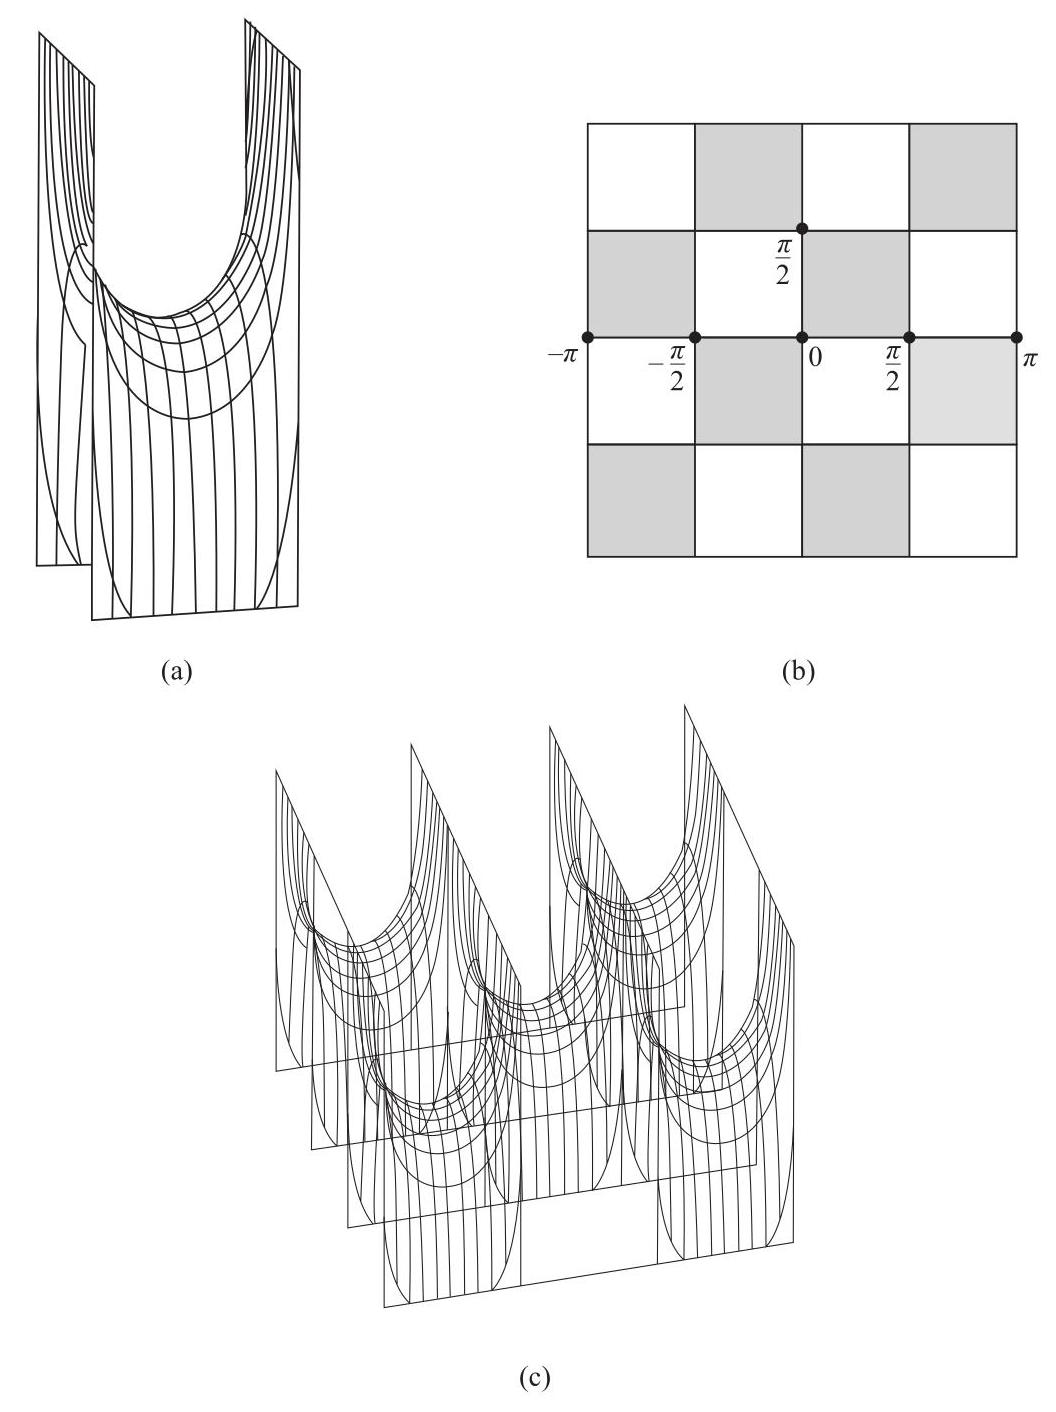
\includegraphics[max width=0.9\textwidth]{images/bo_d4b9jf3ef24c73e0334g_223_230_188_1056_1412_0.jpg}
\end{center}
\hspace*{3em} 

图 3-45.Scherk 曲面.

\exerciseline

1. 证明螺旋面(参见第 2-5 节的示例 3)是一个直纹曲面，其striction 线是 \(z\) 轴，其分布参数是常数.

2. 证明在旋转双曲面 \({x}^{2} + {y}^{2} - {z}^{2} = 1\) 上，半径最小的平行圈是striction 线，其生成线以恒定角度相交，并且分布参数是常数.

3. 设 \(\alpha  : I \rightarrow  S \subset  {R}^{3}\) 是正则曲面 \(S\) 上的一条曲线，并考虑由族 \(\{ \alpha \left( t\right) ,N\left( t\right) \}\) 生成的直纹曲面，其中 \(N\left( t\right)\) 是曲面在 \(\alpha \left( t\right)\) 处的法向量.证明 \(\alpha \left( I\right)  \subset  S\) 是 \(S\) 中的一条曲率线，当且仅当该直纹曲面是可展的.

4. 假设一个非圆柱直纹曲面

\[
\mathbf{x}\left( {t,v}\right)  = \alpha \left( t\right)  + {vw}\left( t\right) ,\;\left| w\right|  = 1,
\]

是正则的.设 \(w\left( {t}_{1}\right) ,w\left( {t}_{2}\right)\) 为两条生成线的 \(\mathbf{x}\) 方向，设 \(\mathbf{x}\left( {{t}_{1},{v}_{1}}\right) ,\mathbf{x}\left( {{t}_{2},{v}_{2}}\right)\) 为这两条生成线的公垂线之足.随着 \({t}_{2} \rightarrow  {t}_{1}\) ，这些点趋于一点 \(\mathbf{x}\left( {{t}_{1},\bar{v}}\right)\) .为了确定 \(\left( {{t}_{1},\bar{v}}\right)\) ，证明以下命题:

a. 公垂线的单位向量收敛于曲面上 \(\left( {{t}_{1},\bar{v}}\right)\) 的切线单位向量.由此得出，在 \(\left( {{t}_{1},\bar{v}}\right)\) 处，

\[
\left\langle  {{w}^{\prime } \land  w,N}\right)  = 0.
\]

b. \(\bar{v} =  - \left( {\left\langle  {{\alpha }^{\prime },{w}^{\prime }}\right\rangle  /\left\langle  {{w}^{\prime },{w}^{\prime }}\right\rangle  }\right)\) .

因此， \(\left( {{t}_{1},\bar{v}}\right)\) 是通过 \({t}_{1}\) 的生成线的中心点，这给出了另一条(假定为非奇异的)屈曲线的解释.

5. 直圆锥面是这样一种生成曲面，其生成线 \({L}_{t}\) 在固定轴 \(r\) 处相互垂直相交，该轴 \(r\) 不与准线 \(\alpha  : I \rightarrow  {R}^{3}\) 相交.

a. 求直圆锥面的参数化方程，并确定一个条件，该条件意味着它不是圆柱面.

b. 给定一个非柱面直锥面，求其严格线和分布参数.

6. 令

\[
\mathbf{x}\left( {t,v}\right)  = \alpha \left( t\right)  + {vw}\left( t\right)
\]

为一个可展曲面.证明在正则点处有

\[
\left\langle  {{N}_{v},{\mathbf{x}}_{v}}\right\rangle   = \left\langle  {{N}_{v},{\mathbf{x}}_{t}}\right\rangle   = 0.
\]

由此得出，可展曲面的切平面在固定母线(的正则点)上是常数.

7. 令 \(S\) 为一个正则曲面，令 \(C \subset  S\) 为 \(S\) 上的一个正则曲线，该曲线在任何地方都不与渐近方向相切.考虑 \(S\) 沿 \(C\) 的切平面族的外包络面.证明通过点 \(p \in  C\) 的母线方向与 \(C\) 在 \(p\) 处的切线方向共轭.

8. 证明如果 \(C \subset  {S}^{2}\) 是单位球面 \({S}^{2}\) 的一个平行曲面，那么 \({S}^{2}\) 沿 \(C\) 的切平面外包络面要么是圆柱面(如果 \(C\) 是赤道)，要么是圆锥面(如果 \(C\) 不是赤道).

9. (焦点曲面.)令 \(S\) 为一个没有抛物点或脐点的正则曲面.令 \(\mathbf{x} : U \rightarrow  S\) 为 \(S\) 的一个参数化，使得坐标曲线是曲率线(如果 \(U\) 很小，这不是限制.参见第 3-4 节推论 4).参数化曲面

\[
\mathbf{y}\left( {u,v}\right)  = \mathbf{x}\left( {u,v}\right)  + {\rho }_{1}N\left( {u,v}\right) ,
\]

\[
\mathbf{z}\left( {u,v}\right)  = \mathbf{x}\left( {u,v}\right)  + {\rho }_{2}N\left( {u,v}\right) ,
\]

其中 \({\rho }_{1} = 1/{k}_{1},{\rho }_{2} = 1/{k}_{2}\) ，称为 \(\mathbf{x}\left( U\right)\) 的焦点曲面(或 \(\mathbf{x}\left( U\right)\) 的中心曲面；这个术语来源于这样一个事实，即 \(\mathbf{y}\left( {u,v}\right)\) ，例如，是 \(\mathbf{x}\left( {u,v}\right)\) 处法截面(参见第 1-6 节练习 2)的中心，该法截面对应于主曲率 \({k}_{1}\) ).证明

a. 如果 \({\left( {k}_{1}\right) }_{u}\) 和 \({\left( {k}_{2}\right) }_{v}\) 处处不为零，则 \(\mathbf{y}\) 和 \(\mathbf{z}\) 是正则参数化曲面.

b. 在正则点处，焦点曲面上的方向对应于 \(\mathbf{x}\left( U\right)\) 上的主方向是共轭的.这意味着，例如，对于所有 \(\left( {u,v}\right)  \in  U\) ， \({\mathbf{y}}_{u}\) 和 \({\mathbf{y}}_{v}\) 在 \(\mathbf{y}\left( U\right)\) 中是共轭向量.

c. 焦点曲面，例如 \(\mathbf{y}\) ，可以构造如下:考虑 \(\mathbf{x}\left( U\right)\) 上的曲率线 \(\mathbf{x}\left( {u\text{ , const. }}\right)\) ，并构造由 \(\mathbf{x}\left( U\right)\) 沿曲线 \(\mathbf{x}\left( {u\text{ , const. }}\right)\) 的法线生成的开发曲面(参见练习 3).这样的开发曲面的严格线位于 \(\mathbf{y}\left( U\right)\) 上，并且当 \(\mathbf{x}\left( {u\text{ , const. }}\right)\) 描述 \(\mathbf{x}\left( U\right)\) 时，这条线描述 \(y\left( U\right)\) (图 3-46).

10. 4. 示例可推广如下.单参数可微平面族 \(\{ \alpha \left( t\right) ,N\left( t\right) \}\) 是一种对应关系，它为每个 \(t \in  I\) 分配一个点 \(\alpha \left( t\right)  \in  {R}^{3}\) 和一个单位向量 \(N\left( t\right)  \in  {R}^{3}\) ，使得 \(\alpha\) 和 \(N\) 都是可微映射.族 \(\{ \alpha \left( t\right) ,N\left( t\right) \} ,t \in  I\) 被称为切平面族，如果对于所有 \(t \in  I\) ，都有 \({\alpha }^{\prime }\left( t\right)  \neq  0,{N}^{\prime }\left( t\right)  \neq  0\) 和 \(\left\langle  {{\alpha }^{\prime }\left( t\right) ,N\left( t\right) }\right\rangle   = 0\) .

a. 证明单参数可微切平面族 \(\{ \alpha \left( t\right) ,N\left( t\right) \}\) 确定一个单参数可微直线族 \(\left\{  {\alpha \left( t\right) ,\left( {N \land  {N}^{\prime }}\right) /\left| {N}^{\prime }\right| }\right\}\) ，该直线族生成一个可展曲面.

\[
\mathbf{x}\left( {t,v}\right)  = \alpha \left( t\right)  + v\frac{N \land  {N}^{\prime }}{\left| {N}^{\prime }\right| }.
\]
 (*)

曲面 \(\left( *\right)\) 称为族 \(\{ \alpha \left( t\right) ,N\left( t\right) \}\) 的包络.

b. 证明如果对于所有 \(t \in  I\) ，都有 \({\alpha }^{\prime }\left( t\right)  \land  \left( {N\left( t\right)  \land  {N}^{\prime }\left( t\right) }\right)  \neq  0\) ，则包络 (*) 在 \(v = 0\) 的邻域内是正则的，并且 \(\mathbf{x}\) 在 \(\left( {t,0}\right)\) 处的单位法向量是 \(N\left( t\right)\) .

c. 令 \(\alpha  = \alpha \left( s\right)\) 为 \({R}^{3}\) 中的一条曲线，由弧长参数化.假设 \(\alpha\) 的曲率 \(k\left( s\right)\) 和挠率 \(\tau \left( s\right)\) 处处不为零.

\begin{center}
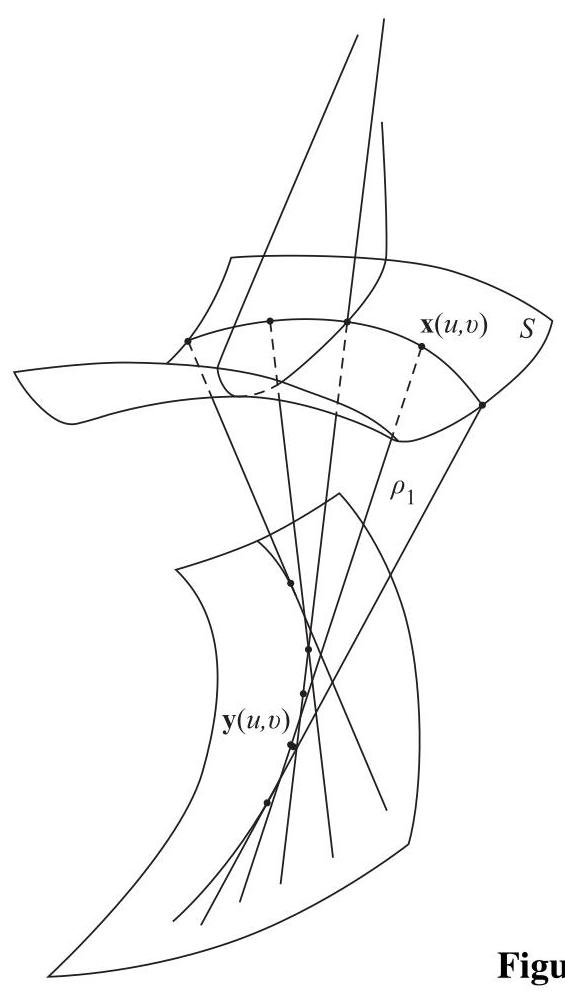
\includegraphics[max width=0.5\textwidth]{images/bo_d4b9jf3ef24c73e0334g_226_196_186_565_993_0.jpg}
\end{center}
\hspace*{3em} 

图 3-46. 焦点曲面的构造.

证明密切平面族 \(\{ \alpha \left( s\right) ,b\{ s\} \}\) 是单参数可微切平面族，并且该族的包络是 \(\alpha \left( s\right)\) 的切面(参见 5. 示例，第 2-3 节).

11. 令 \(\mathbf{x} = \mathbf{x}\left( {u,v}\right)\) 为一个正则参数化曲面.与 \(\mathbf{x}\) 平行的曲面是一个参数化曲面

\[
\mathbf{y}\left( {u,v}\right)  = \mathbf{x}\left( {u,v}\right)  + {aN}\left( {u,v}\right) ,
\]

其中 \(a\) 是一个常数.

a. 证明 \({y}_{u} \land  {y}_{v} = \left( {1 - {2Ha} + K{a}^{2}}\right) \left( {{\mathbf{x}}_{u} \land  {\mathbf{x}}_{v}}\right)\) ，其中 \(K\) 和 \(H\) 分别是 \(\mathbf{x}\) 的高斯曲率和平均曲率.

b. 证明在正则点处， \(\mathbf{y}\) 的高斯曲率是

\[
\frac{K}{1 - {2Ha} + K{a}^{2}}
\]

并且 \(\mathbf{y}\) 的平均曲率是

\[
\frac{H - {Ka}}{1 - {2Ha} + K{a}^{2}}.
\]

c. 令曲面 \(\mathbf{x}\) 具有等于 \(c \neq  0\) 的常平均曲率，并考虑距离为 \(1/{2c}\) 的 \(\mathbf{x}\) 的平行曲面.证明该平行曲面具有等于 \(4{c}^{2}\) 的常高斯曲率.

12. 证明不存在紧致的(即在 \({R}^{3}\) 中有界且闭合的)极小曲面.

13. a. 设 \(S\) 为一个没有脐点的正则曲面.证明 \(S\) 是极小曲面当且仅当高斯映射 \(N : S \rightarrow  {S}^{2}\) 对所有 \(p \in  S\) 和所有 \({w}_{1},{w}_{2} \in  {T}_{p}\left( S\right)\) 满足:

\[
{\left\langle  d{N}_{p}\left( {w}_{1}\right) ,d{N}_{p}\left( {w}_{2}\right) \right\rangle  }_{N\left( p\right) } = \lambda \left( p\right) {\left\langle  {w}_{1},{w}_{2}\right\rangle  }_{p},
\]

其中 \(\lambda \left( p\right)  \neq  0\) 是一个仅取决于 \(p\) 的数.

b. 设 \(\mathbf{x} : U \rightarrow  {S}^{2}\) 是单位球面 \({S}^{2}\) 通过立体投影的参数化.考虑 a 部分的极小曲面 \(S\) 的一点 \(p\) 的邻域 \(V\) ，使得 \(N : S \rightarrow  {S}^{2}\) 在 \(V\) 上的限制是一个微分同胚(因为 \(K\left( p\right)  = \det \left( {d{N}_{p}}\right)  \neq  0\) ，根据反函数定理存在这样的 \(V\) ).证明参数化 \(y = {N}^{-1} \circ \; \mathbf{x} : U \rightarrow  S\) 是等温的(这提供了一种在没有平面点的情况下在极小曲面上引入等温参数化的方法).

14. 当两个可微函数 \(f,g : U \subset  {R}^{2} \rightarrow  R\) 满足柯西-黎曼方程时

\[
\frac{\partial f}{\partial u} = \frac{\partial g}{\partial v},\;\frac{\partial f}{\partial v} =  - \frac{\partial g}{\partial u},
\]

它们很容易被看出是调和的；在这种情况下， \(f\) 和 \(g\) 被称为调和共轭.设 \(\mathbf{x}\) 和 \(\mathbf{y}\) 是极小曲面的等温参数化，使得它们的成分函数成对地是调和共轭的；那么 \(\mathbf{x}\) 和 \(\mathbf{y}\) 被称为共轭极小曲面.证明:

a. 螺旋面和链面是共轭极小曲面.

b. 给定两个共轭极小曲面 \(\mathbf{x}\) 和 \(\mathbf{y}\) ，曲面

\[
\mathbf{z} = \left( {\cos t}\right) \mathbf{x} + \left( {\sin t}\right) \mathbf{y}
\]
 (*)

对于所有 \(t \in  R\) 仍然是极小的.

c. 一参数族 \(\left( *\right)\) 的所有曲面都具有相同的基本形式: \(E = \left\langle  {{\mathbf{x}}_{u},{\mathbf{x}}_{u}}\right\rangle   = \left\langle  {{\mathbf{y}}_{v},{\mathbf{y}}_{v}}\right\rangle  ,F = 0,G = \left\langle  {{\mathbf{x}}_{v},{\mathbf{x}}_{v}}\right\rangle   = \left\langle  {{\mathbf{y}}_{u},{\mathbf{y}}_{u}}\right\rangle\) .

因此，任何两个共轭极小曲面都可以通过一个一参数的极小曲面族连接起来，并且该族的第一基本形式与 \(t\) 无关.

附录 自伴线性映射和二次型

在本附录中， \(V\) 表示一个二维向量空间，带有一个内积 \(\langle\) ， \(\rangle {.Allthatfollowsaanbeeasilyextendedtoafinite} \; n\) 维向量空间，但为了简单起见，我们只讨论 \(n = 2\) 的情况.

我们说一个线性映射 \(A : V \rightarrow  V\) 是自伴的，如果对于所有 \(v,w \in  V\) 都有 \(\langle {Av},w\rangle  = \langle v,{Aw}\rangle\) .

注意到，如果 \(\left\{  {{e}_{1},{e}_{2}}\right\}\) 是 \(V\) 和 \(\left( {\alpha }_{ij}\right) ,i,j = 1,2\) 的一个标准正交基， \(\left( {\alpha }_{ij}\right) ,i,j = 1,2\) 是该基下的 \(A\) 的矩阵，那么

\[
\left\langle  {A{e}_{j},{e}_{i}}\right\rangle   = {\alpha }_{ij} = \left\langle  {{e}_{j},A{e}_{i}}\right\rangle   = \left\langle  {A{e}_{i},{e}_{j}}\right\rangle   = {\alpha }_{ji};
\]

也就是说，矩阵 \(\left( {\alpha }_{ij}\right)\) 是对称的.

我们为每个自伴线性映射关联一个由下式定义的映射 \(B : V \times  V \rightarrow  R\) :

\[
B\left( {v,w}\right)  = \langle {Av},w\rangle .
\]

\(B\) 显然是双线性的；也就是说，它在 \(v\) 和 \(w\) 上都是线性的.此外， \(A\) 是自伴的事实意味着 \(B\left( {v,w}\right)  = B\left( {w,v}\right)\) ；也就是说， \(B\) 是 \(V\) 中的一个对称双线性形式.

反之，如果 \(B\) 是 \(V\) 中的一个对称双线性形式，我们可以定义一个线性映射 \(A : V \rightarrow  V\) ，由 \(\langle {Av},w\rangle  = B\left( {v,w}\right)\) 定义，并且 \(B\) 的对称性意味着 \(A\) 是自伴的.

另一方面，对于 \(V\) 中的每个对称双线性形式 \(B\) ，都存在一个 \(V\) 中的二次型 \(Q\) ，由下式给出:

\[
Q\left( v\right)  = B\left( {v,v}\right) ,\;v \in  V,
\]

并且 \(Q\) 的知识完全确定了 \(B\) ，因为

\[
B\left( {u,v}\right)  = \frac{1}{2}\left\lbrack  {Q\left( {u + v}\right)  - Q\left( u\right)  - Q\left( v\right) }\right\rbrack  .
\]

因此，在 \(V\) 中的二次型和 \(V\) 的自伴线性映射之间建立了一一对应关系.

本附录的目的是证明(参见下面的定理)，给定一个自伴线性映射 \(A : V \rightarrow  V\) ，存在一个 \(V\) 的标准正交基，使得相对于该基， \(A\) 的矩阵是一个对角矩阵.此外，对角线上的元素是 \(V\) 的单位圆上相应二次型的最大值和最小值.

引理.如果函数 \(\mathrm{Q}\left( {x,\mathrm{y}}\right)  = {\mathrm{{ax}}}^{2} + 2\mathrm{{bxy}} + {\mathrm{{cy}}}^{2}\) 在单位圆 \({x}^{2} + {\mathrm{y}}^{2} = 1\) 上受限，在点 \(\left( {1,0}\right)\) 处取得最大值，则 \(\mathrm{b} = 0\) .

证明.用 \(x = \cos t,\;y = \sin t\) 和 \(t \in  \left( {0 - \epsilon ,{2\pi } + \epsilon }\right)\) 参数化圆 \({x}^{2} + {y}^{2} = 1\) .因此， \(Q\) 在该圆上受限后，成为一个关于 \(t\) 的函数:

\[
Q\left( t\right)  = a{\cos }^{2}t + {2b}\cos t\sin t + c{\sin }^{2}t.
\]

由于 \(Q\) 在点 \(\left( {1,0}\right)\) 处取得最大值，我们有

\[
{\left( \frac{dQ}{dt}\right) }_{t = 0} = {2b} = 0.
\]

因此， \(b = 0\) 如我们所愿.Q.E.D.

命题.给定 \(\mathrm{V}\) 中的一个二次型 \(\mathrm{Q}\) ，存在一个 \(\mathrm{V}\) 的标准正交基 \(\left\{  {{e}_{1},{e}_{2}}\right\}\) ，使得如果 \(\mathrm{v} \in  \mathrm{V}\) 由 \(\mathrm{v} = {\mathrm{{xe}}}_{1} + {\mathrm{{ye}}}_{2}\) 定义，则

\[
\mathrm{Q}\left( \mathrm{v}\right)  = {\lambda }_{1}{x}^{2} + {\lambda }_{2}{\mathrm{y}}^{2},
\]

其中 \({\lambda }_{1}\) 和 \({\lambda }_{2}\) 分别是 \(\mathrm{Q}\) 在单位圆 \(\left| \mathrm{v}\right|  = 1\) 上的最大值和最小值.

证明.设 \({\lambda }_{1}\) 是 \(Q\) 在单位圆 \(\left| v\right|  = 1\) 上的最大值，设 \({e}_{1}\) 是一个单位向量，使得 \(Q\left( {e}_{1}\right)  = {\lambda }_{1}\) .由于 \(Q\) 在紧集 \(\left| v\right|  = 1\) 上是连续的，这样的 \({e}_{1}\) 存在.设 \({e}_{2}\) 是一个与 \({e}_{1}\) 正交的单位向量，并令 \({\lambda }_{2} = Q\left( {e}_{2}\right)\) .我们将证明基 \(\left\{  {{e}_{1},{e}_{2}}\right\}\) 满足命题的条件.

令 \(B\) 为与 \(Q\) 相关联的对称双线性形式，并设 \(v = \; x{e}_{1} + y{e}_{2}\) .则

\[
Q\left( v\right)  = B\left( {v,v}\right)  = B\left( {x{e}_{1} + y{e}_{2},x{e}_{1} + y{e}_{2}}\right)
\]

\[
= {\lambda }_{1}{x}^{2} + {2bxy} + {\lambda }_{2}{y}^{2},
\]

其中 \(b = B\left( {{e}_{1},{e}_{2}}\right)\) .根据引理， \(b = 0\) ，并且只剩下证明 \({\lambda }_{2}\) 是 \(Q\) 在圆 \(\left| v\right|  = 1\) 上的最小值.这很直接，因为对于任何具有 \({x}^{2} + {y}^{2} = 1\) 的 \(v = x{e}_{1} + y{e}_{2}\) ，我们有

\[
Q\left( v\right)  = {\lambda }_{1}{x}^{2} + {\lambda }_{2}{y}^{2} \geq  {\lambda }_{2}\left( {{x}^{2} + {y}^{2}}\right)  = {\lambda }_{2},
\]

因为 \({\lambda }_{2} \leq  {\lambda }_{1}\) .Q.E.D.

我们称向量 \(v \neq  0\) 是线性映射 \(A : V \rightarrow  V\) 的一个特征向量，如果存在一个实数 \(\lambda ;\lambda\) 使得 \({Av} = {\lambda v}\) ，则该实数被称为 \(A\) 的一个特征值.

定理.设 A: \(\mathrm{V} \rightarrow  \mathrm{V}\) 是一个自伴线性映射.则存在 \(\mathrm{V}\) 的一个标准正交基 \(\left\{  {{e}_{1},{e}_{2}}\right\}\) ，使得 \(\mathrm{A}\left( {\mathrm{e}}_{1}\right)  = {\lambda }_{1}{\mathrm{e}}_{1},\mathrm{\;A}\left( {\mathrm{e}}_{2}\right)  = {\lambda }_{2}{\mathrm{e}}_{2}\) (即， \({\mathrm{e}}_{1}\) 和 \({\mathrm{e}}_{2}\) 是 \(\mathrm{A}\) 的特征向量，而 \({\lambda }_{1},{\lambda }_{2}\) 是特征值).在基 \(\left\{  {{e}_{1},{e}_{2}}\right\}\) 中， \(\mathrm{A}\) 的矩阵显然是对角矩阵，并且对角线上的元素 \({\lambda }_{1},{\lambda }_{2}\) 和 \({\lambda }_{1} \geq  {\lambda }_{2}\) 分别是二次型 \(\mathrm{Q}\left( \mathrm{v}\right)  = \langle \mathrm{{Av}},\mathrm{v}\rangle\) 在 \(\mathrm{V}\) 的单位圆上的最大值和最小值.

证明.考虑二次型 \(Q\left( v\right)  = \langle {Av},v\rangle\) .根据上述命题，存在 \(V\) 的一个标准正交基 \(\left\{  {{e}_{1},{e}_{2}}\right\}\) ，其中 \(Q\left( {e}_{1}\right)  = {\lambda }_{1}\) ， \(Q\left( {e}_{2}\right)  = {\lambda }_{2} \leq  {\lambda }_{1}\) ，其中 \({\lambda }_{1}\) 和 \({\lambda }_{2}\) 分别是 \(Q\) 在单位圆上的最大值和最小值.因此，只剩下证明

\[
A\left( {e}_{1}\right)  = {\lambda }_{1}{e}_{1},\;A\left( {e}_{2}\right)  = {\lambda }_{2}\left( {e}_{2}\right) .
\]

根据 \(B\left( {{e}_{1},{e}_{2}}\right)  = \left\langle  {A{e}_{1},{e}_{2}}\right\rangle   = 0\) (由引理可知)和 \({e}_{2} \neq  0\) ，我们得到 \(A{e}_{1}\) 平行于 \({e}_{1}\) 或 \(A{e}_{1} = 0\) .如果 \(A{e}_{1}\) 平行于 \({e}_{1}\) ，则 \(A{e}_{1} = \alpha {e}_{1}\) ，并且由于 \(\left\langle  {A{e}_{1},{e}_{1}}\right\rangle   = {\lambda }_{1} = \left\langle  {\alpha {e}_{1},{e}_{2}}\right\rangle   = \alpha\) ，我们得出 \(A{e}_{1} = {\lambda }_{1}{e}_{1}\) ；如果 \(A{e}_{1} = 0\) ，则 \({\lambda }_{1} = \left\langle  {A{e}_{1},{e}_{1}}\right\rangle   = 0\) ，并且 \(A{e}_{1} = 0 = {\lambda }_{1}{e}_{1}\) .因此，在任何情况下，我们都有 \(A{e}_{1} = {\lambda }_{1}{e}_{1}\) .

现在利用以下事实:

\[
B\left( {{e}_{1},{e}_{2}}\right)  = \left\langle  {A{e}_{2},{e}_{1}}\right\rangle   = 0
\]

以及

\[
\left\langle  {A{e}_{2},{e}_{2}}\right\rangle   = {\lambda }_{2},
\]

我们可以用同样的方式证明 \(A{e}_{2} = {\lambda }_{2}{e}_{2}\) .Q.E.D.

注.将上述结果推广到 \(n\) 维向量空间 \(n > 2\) ，只需要采取以下预防措施.在前面的命题中，我们在单位球上选择 \(Q\) 的最大 \({\lambda }_{1} = Q\left( {e}_{1}\right)\) ，然后证明 \(Q\) 在垂直于 \({e}_{1}\) 的子空间 \({V}_{1}\) 中限制为一个二次型 \({Q}_{1}\) .我们选择 \({V}_{1}\) 单位球上 \({Q}_{1}\) 的最大值作为 \({\lambda }_{2} = {Q}_{1}\left( {e}_{2}\right)\) ，依此类推.
